\documentclass[10pt,portrait, twocolumn]{article}
\usepackage{multicol}
\usepackage{calc}
\usepackage[portrait]{geometry}
\usepackage{amsmath,amsthm,amsfonts,amssymb}
\usepackage{times}
\usepackage{color,graphicx,overpic}
\graphicspath{ {images/} }
\usepackage{hyperref}
\usepackage{pgfplots}
\usepackage{esint}
\usepackage{bm}
\usepackage{tikz}
\usepackage{relsize}
\usepackage{datetime}
\usepackage[utf8] {inputenc}
\usepackage[spanish, activeacute] {babel}
\usepackage{IEEEtrantools}
\usepackage{framed}

\usepackage{pdflscape}

%\usepackage{draftwatermark}
%\SetWatermarkText{Javier de Martín}
%\SetWatermarkScale{0.8}

% This sets page margins to .5 inch if using letter paper, and to 1cm
% if using A4 paper. (This probably isn't strictly necessary.)
% If using another size paper, use default 1cm margins.
\geometry{top=.5cm,left=.5cm,right=.5cm,bottom=.5cm}
    
\pgfplotsset{
    dirac/.style={
        mark=triangle*,
        mark options={scale=2},
        ycomb,
        scatter,
        visualization depends on={y/abs(y)-1 \as \sign},
        scatter/@pre marker code/.code={\scope[rotate=90*\sign,yshift=-2pt]}
    }
}

% Turn off header and footer
\pagestyle{empty}

% Redefine section commands to use less space
\makeatletter
\renewcommand{\section}{\@startsection{section}{1}{0mm}%
                                {-1ex plus -.5ex minus -.2ex}%
                                {0.5ex plus .2ex}%x
                                {\normalfont\large\bfseries}}
\renewcommand{\subsection}{\@startsection{subsection}{2}{0mm}%
                                {-1explus -.5ex minus -.2ex}%
                                {0.5ex plus .2ex}%
                                {\normalfont\normalsize\bfseries}}
\renewcommand{\subsubsection}{\@startsection{subsubsection}{3}{0mm}%
                                {-1ex plus -.5ex minus -.2ex}%
                                {1ex plus .2ex}%
                                {\normalfont\small\bfseries}}
\makeatother

\newcommand{\Lagr}{\mathcal{L}}

% Define BibTeX command
\def\BibTeX{{\rm B\kern-.05em{\sc i\kern-.025em b}\kern-.08em
    T\kern-.1667em\lower.7ex\hbox{E}\kern-.125emX}}

% Don't print section numbers
\setcounter{secnumdepth}{5}


\setlength{\parindent}{0pt}
\setlength{\parskip}{0pt plus 0.5ex}

%My Environments
\newtheorem{example}[section]{Example}
% ---------------------------------------------------------------

\begin{document}


\begin{framed}
	\begin{center}
    	\Large{\underline{Redes de Transporte}} \\
    	\scriptsize{3º Ingeniería de Telecomunicaciones | UPV/EHU}\\
     	%Actualizado por última vez el \today \\
     	"\textsl{Under-promise and over-deliver}." \\
     	%\hspace{5 pt} \\
     	\small{\textbf{Javier de Martín -- 2016}}
	\end{center}
\end{framed}

%%%%%%%%%%%%%%%%%%%%%%%%%%%%%%%%%%%%%%%%%%%%%%%%%%%%%%%%%%%%%%%%%
% Tema 4
\textbf{Revisar 1.1 y 1.2}

\begin{center}
\section{\underline{0.- Introducción}}
\end{center}

Las redes de \textbf{acceso} hacen llegar la información del origen al primer equipo de red. Las redes de \textbf{transporte} llevan la información a través de la red, realiza las tareas de conmutación (nivel 2) y encaminamiento (nivel 3), transmisión y señalización.

\hrulefill

\section{\underline{1.- Encaminamiento}}

\textbf{Encaminar} consiste en establecer una ruta óptima para una instancia de comunicación desde una fuente a un destino. La ruta elegida debe optimizar en lo posible algún parámetro o conjunto de ellos. Las decisiones de encaminamiento son incrementales, cada nodo sólo debe decidir a qué nodo adyacente debe transmitir los datos.

\begin{itemize}
	\item \textbf{Algoritmo de encaminamiento}: Dado un destino decide la línea de salida adecuada.
	\item \textbf{Tabla de encaminamiento}: Estructura de información donde almacenar localmente los pares destino-salida.
	\item \textbf{Protocolo de encaminamiento}: Coordinación entre nodos del cálculo de las rutas e informar de entre sí de los cambios que se produzcan, por ejemplo, en la topología de la red.
\end{itemize}

Los encaminamientos deben de ser \textbf{robustos} para adaptarse a los posibles cambios de topología sin necesidad de abortar o reiniciar la red, \textbf{estables} en el sentido de converger a un resultado lo más rápido posible, no deben de generar \textbf{bucles} en el encaminamiento y no deben \textbf{favorecer} a ningún usuario frente a otro sin motivo.

\subsection{Encaminamiento IP}

En función de \textbf{dónde se decide encaminar}:

	\begin{itemize}
		\item \textbf{Fijado en el origen (Source Routing)}: Son los sistemas finales los que fijan la ruta que ha de seguir cada paquete. Cada paquete lleva un campo que especifica su ruta (RI, Routing Information), y los nodos sólo se dedican a reenviar los paquetes por esas rutas ya especificadas. Los sistemas finales son los que tienen las tablas de encaminamiento y no se hace necesaria la consulta o existencia de tablas de encaminamiento en los nodos intermedios. El nodo origen debe de conocer la topología de la red. No existen bucles, el sistema final fija la ruta.
		\item \textbf{Salto a Salto (Hop by Hop)}: Los nodos, en función del destino, conocen sólo el siguiente salto a realizar. Pueden ocurrir bucles, no se tiene una visión completa de la red.
	\end{itemize}
	
En función de la \textbf{adaptabilidad}:

	\begin{itemize}
		\item \textbf{No adaptables (estáticos)}:
			\begin{itemize}
				\item Estáticos: Las tablas de encaminamiento de los nodos se configuran de forma manual y permanecen inalterables hasta que no se vuelve a actuar sobre ellas. Tanto la recogida como la distribución de información se realiza por gestión (manera externa a la red), sin ocupar capacidad de red. Es óptimo para topologías de red en las que sólo hay una posibilidad de encaminamiento (topología en estrella).
				\item Q-Estáticos: Igual que el estático pero en vez de dar una sola ruta fija se proporcionan varias alternativas en caso de que la principal no funcione. Tiene adaptabilidad reducida.
			\end{itemize}
		\item \textbf{Adaptables (dinámicos)}:
			\begin{itemize}
				\item Centralizados: Los nodos envían a un nodo central la información de control acerca de sus vecinos. El nodo central será el que se encargue de recoger esta información de control acerca de sus vecinos. El nodo central será el que se encargue de recoger esta información para construir la tabla de encaminamiento de cada nodo en función de la información de control que éstos le mandan. Tiene un alto consumo de recursos de la red y se necesita disponer de rutas alternativas (y nodo central alternativo) para comunicarse con el nodo central, ya que estos métodos dejarían de funcionar con la caída de éste.
				\item Aislados: El más simple, no tiene en cuenta la información de los otros nodos a la hora de encaminar. Cada vez que un nodo recibe un paquete que tiene que reenviar (porque no es para él) lo reenvía por todos los enlaces salvo por el que le llegó (inundación). Útil para enviar información de emergencia ya que se asegura que llega a todos los nodos.
				\item Distribuidos: Todos los nodos son iguales, todos envían y reciben información de control y todos calculan, a partir de su RIB (base de información de encaminamiento) sus tablas de encaminamiento. La adaptación a cambios es óptima siempre y cuando éstos sean notificados.
			\end{itemize}
	\end{itemize}

\begin{center}
\begin{tabular}{|l|l|l|l|}
\hline
\textbf{Encaminamiento} & \textbf{Info de Control} & \textbf{Decisión} & \textbf{Adaptación} \\ \hline
\textbf{Estáticos}               & No                              & Offline                             & No                                \\ \hline
\textbf{Cuasiestáticos}          & No                              & Offline                             & Reducida                          \\ \hline
\textbf{Centralizado}            & Nodo Central                    & Nodo Central                        & Si                                \\ \hline
\textbf{Distribuido}             & Entre Nodos                     & Cada Nodo                           & Si                                \\ \hline
\textbf{Aislado}                 & no                              & Cada Nodo                           & Si                                \\ \hline
\end{tabular}
\end{center}

En el encaminamiento \textbf{estático} la tabla de encaminamiento de los equipos se actualiza de forma manual y en el \textbf{dinámico} se actualiza mediante protocolos de encaminamiento.

\subsection{Encaminadores o Routers}

Un \textbf{router} tiene que encontrar una ruta y encaminar los datos. \textit{Routing} es el proceso de decidir a dónde enviar un paquete recibido utilizando la tabla de encaminamiento del router y \textit{forwarding} es el acto de enviar el paquete al siguiente salto.\\

Los routers tienen dos tablas clave:

	\begin{itemize}
		\item \textbf{FIB} (Forwarding table): Contiene destinos y las interfaces para llegar a ellos. El router la utilizar para descubrir la interfaz a la que enviar los paquetes. A veces se confunden con rutas (\textbf{no entiendo esto}).
		\item \textbf{RIB} (Routing table): Contiene una lista de los destinos alcanzables y los siguientes saltos para alcanzar los destinos. Un destino puede ser alcanzado a través de varios posibles next hops pero sólo el mejor va a la FIB.
	\end{itemize}
	
	\begin{center}
		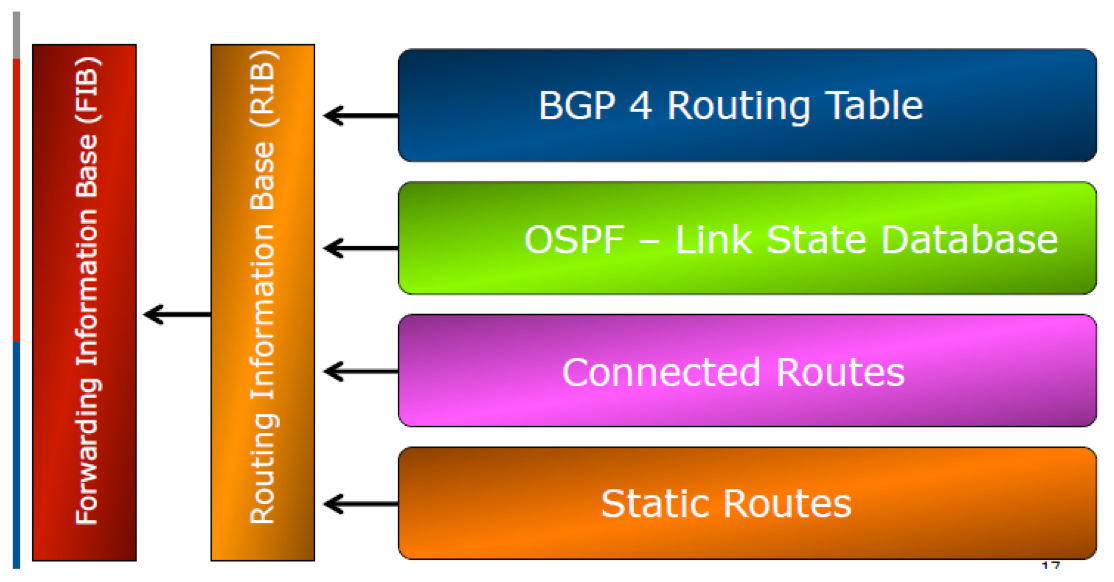
\includegraphics[scale = .5]{FIBRIB}
	\end{center}
	
\subsection{Encaminamiento IP}

El protocolo IP es un protocolo \textbf{no fiable} (best effort), \textbf{no orientado a conexión}, no mantiene \textbf{información de estado}, los datagramas pueden llegar fuera de secuencia con errores o pérdidas, es el protocolo de nivel superior el encargado de resolver estos problemas. \\

IP realiza tiene dos tipos de encaminamiento:

	\begin{itemize}
		\item \textbf{Directo}: Un equipo puede enviar un paquete IP a otra máquina sin pasar por un tercer equipo. En la misma red.
		\item \textbf{Indirecto}: Un equipo quiere enviar un paquete IP a otro equipo y tiene que atravesar una ruta de otros equipos. En distintas redes.
	\end{itemize}

La tabla de encaminamiento IP en cada equipo incluye un conjunto de direcciones IP destino y las direcciones IP del siguiente salto para cada destino. Además, pueden incluir para llegar a destinos rutas directas, indirectas o por defecto. \\

El algoritmo de encaminamiento IP es el siguiente:
	\begin{center}
		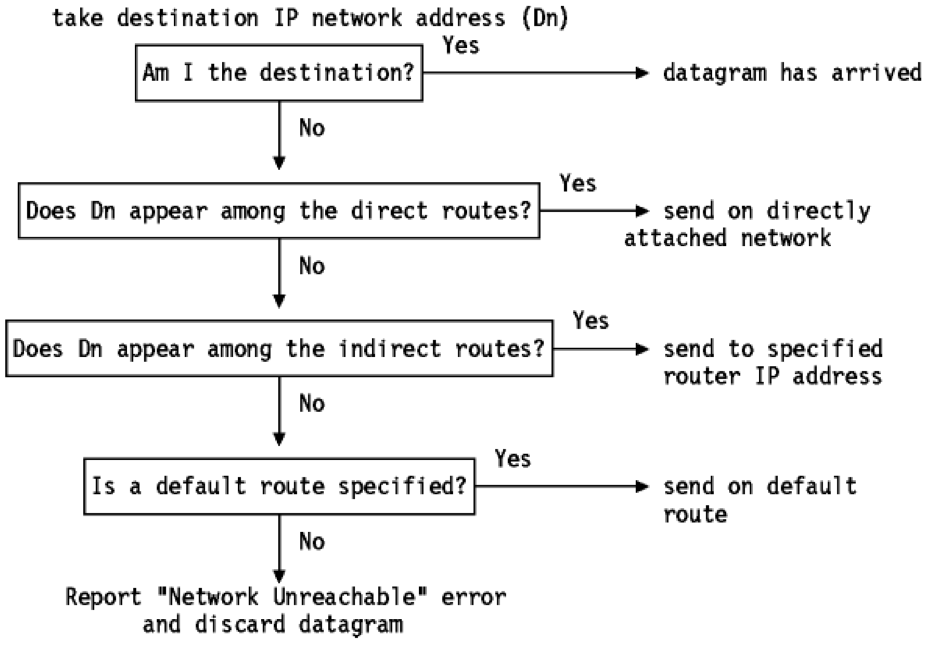
\includegraphics[scale = .5]{AlgoritmoIP}
	\end{center}

\subsection{Encaminamiento en Internet}

Para entender el encaminamiento en internet hay que conocer algunos \textbf{aspectos clave}.  La transmisión es \textbf{no orientada a conexión}, cada router toma decisiones de forma \textbf{local} para encaminar los paquetes hasta el destino. Internet no es una única red sino una colección de reds interconectadas perteneciente a distintos propietarios. Internet se divide en \textbf{Sistemas Autónomos} que está formado por routers, equipos y redes gestionados por una misma administración. Cada Sistema Autónomo se identifica mediante un AS Number que es de 32 bits (antiguamente de 16) y es asignado por las autoridades de numeración de Internet. La división de Internet en Sistemas Autónomos tiene ventajas como la autonomía, disminuye los \textit{overheads} derivados de operaciones de control (encaminamiento), facilita la gestión de las redes...

Los \textbf{protocolos de encaminamiento} permiten la actualización de información de forma dinámica intercambiando información. Hay dos tipos de protocolos de encaminamiento:

	\begin{itemize}
		\item \textbf{IGP} (Interior Gateway Protocol): Operan dentro de un Sistema Autónomo (intra-domain routing), los mensajes IGP se intercambian entre routers que pertenecen a un mismo SA. Cada SA, normalmente, tendrá su propia política de encaminamiento.
		\item \textbf{EGP} (Exterior Gateway Protocol): (inter-domain routing) Permiten intercambio de información entre Sistemas Autónomos.
	\end{itemize}
	
	\begin{itemize}
		\item \textbf{Intradomain Routing}: Encaminamiento dentro de un AS. No tiene en cuenta lo que hay, Internet, fuera del propio AS.
		\item \textbf{Interdomain Routing}: Encaminamiento entre AS. Considera Internet como un conjunto de AS interconectados. Normalmente hay un router en cada AS que maneja tráfico interdomain.
	\end{itemize}
	
	\begin{center}
		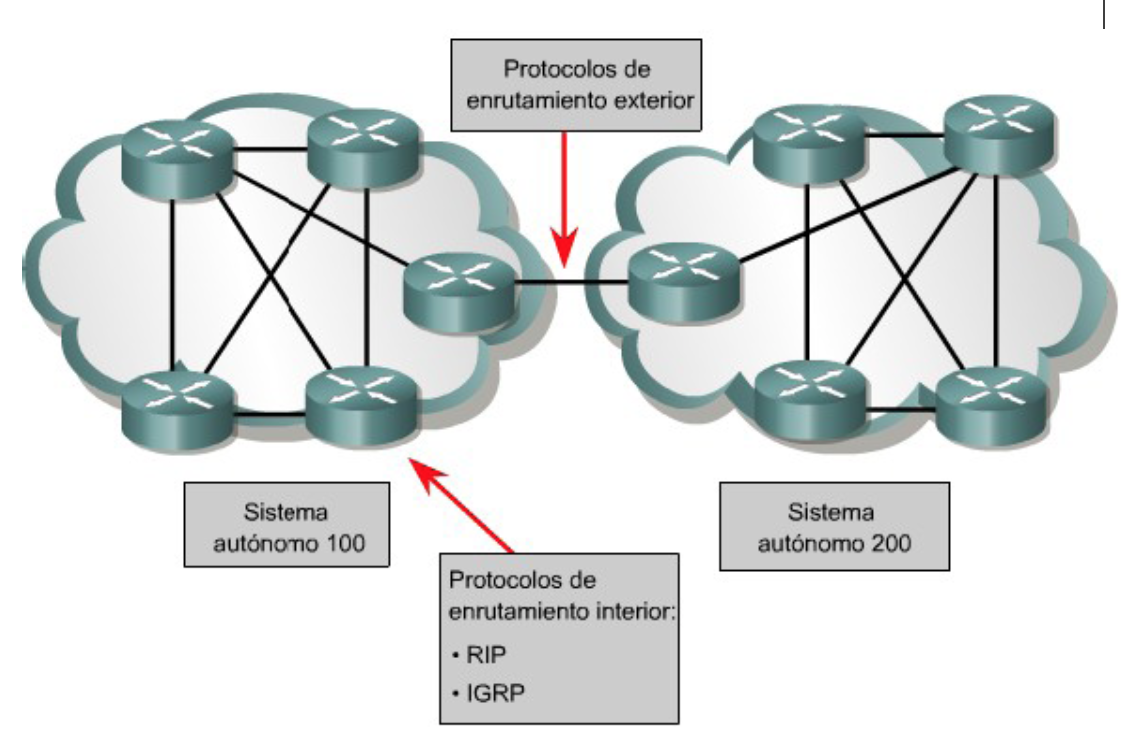
\includegraphics[scale = .5]{InterIntra}
	\end{center}
	
El \textbf{encaminamiento IGP} en redes actuales suele basarse en una combinación de protocolos de encaminamiento dinámicos y rutas estáticas. Cada escenario (parte de una red) tiene diferentes requerimientos. El \textbf{encaminamiento estático} es adecuado cuando hay pocas alternativas (rutas) para elegir que no cambian mucho, por ejemplo cuando un router conecta a una red a Internet o habitual en equipos finales. En equipos IP normalmente consiste en introducir manualmente \texttt{IP address/subnet mask + gateway}. Los protocolos de \textbf{encaminamiento dinámico} comparten la información entre routers, actualizan los encaminamientos cuando se producen cambios en la topología (cambio de rutado), determinan la mejor ruta a cada destino, aprenden información de nuevas redes y destinos y encuentran rutas alternativas en caso de fallos. Sus \textbf{componentes}:

	\begin{itemize}
		\item Estructuras de datos
		\item Algoritmos
		\item Mensajes de Protocolo
		\item Terminar
	\end{itemize}
	
\textbf{Ventajas} rutado estático:
	\begin{itemize}
		\item Mínimo procesado de CPU.
		\item Fácil de entender y administrar.
		\item Fácil de configurar
		\item No requiere recursos extra
		\item Más seguro 
	\end{itemize}
	
\textbf{Desventajas} rutado estático:

	\begin{itemize}
		\item Los cambios en la red requieren reconfiguración manual.
		\item La configuración y mantenimiento son time-consuming.
		\item No escala bien en topologías grandes.
		\item Configuraciones error-prone, especialmente en redes grandes.
	\end{itemize}

\textbf{Ventajas} rutado dinámico:

	\begin{itemize}
		\item El administrado rtiene menos tareas de configuración cuando se añaden o quitan redes nuevas.
		\item Los protocolos reaccionan automáticamente ante cambios de la topología.
		\item La configuración es menos error-prone.
		\item Más escalable.
	\end{itemize}

\textbf{Desventajas} rutado dinámico:

	\begin{itemize}
		\item Uso de recursos de los routers.
		\item Se requieren más conocimientos de administración de red...
	\end{itemize}
	
Tipos de protocolos de encaminamiento IGP (Interior Gateway Protocol) se dividen en dos grupos grandes:

	\begin{itemize}
		\item Distance Vector Routing Protocols: RIPv1 y IGRP.
		\item Link-State Routing Protocols: OSPF, IS-IS.
	\end{itemize}

Cuando se selecciona un protocolo para un caso u otro  hay que fijarse en ciertos criterios: como el tiempo de convergencia, escalabilidad, utilización de recursos, implementación y mantenimiento...\\

Hay que entender un concepto clave, la \textbf{métrica} es el coste asociado a una ruta. Los protocolos utilizan métricas para evaluar, diferenciar y seleccionar entre rutas a destinos. Cada protocolo utiliza distintos tipos de métricas. Hay protocolos que soportan la utilización de varias métricas a la vez. También se pueden configurar costes de forma manual. La métrica total de una ruta es igual a la suma de métricas de todos los enlaces (redes) que componen la ruta.\\

Los algoritmos de vector distancia se basan en el algoritmo de Bellman-Ford para calcular la mejor ruta al destino. Los routers no tienen información completa sobre la topología de la red, sólo conocen la interfaz de salida o dirección del siguiente router para cada destino. Suelen hacer envíos periódicos de vectores distancia a todos los vecinos conectados. \textbf{Funcionamiento}, cada router conoce a sus vecinos y sus enlaces hasta los vecinos. Cada router envía información de su tabla de encmainamiento que se anuncia como vectores de pares.

SALTO HASTA LA PAGINA 30

La \textbf{convergencia} es el estado de una red cuando las tablas de encaminamiento de los routers son consistentes. El \textbf{tiempo de convergencia} es el tiempo que transcurre cuando los routers intercambian información de sus tablas de encaminamiento, calculan las mejores rutas a los destinos, actualizan las tabals de encaminamiento (si es necesario) y construyen y envían los correspondientes VD si es necesario. Es un parámetro importante para caracterizar los protocolos de encaminamiento, cuanto más rápido se alcanza la convergencia mejor es el protocolo de routing.\\

\textbf{¿Cuándo se envían los vectores distancia?} Se hacen actualizaciones periódicas, haciendo algunos protocolos con reconocimiento. Triggered updates, los nodos envían vectores cuando detectan algún cambio en su tabla de encaminamiento después de una actualización por recepción de VD o cuando detectan algún fallo en algún enlace (o enlace nuevo).\\

\textbf{Fallo en un enlace/nodo)}, ¿cómo detectarlo? No llegan los envíos periódicos o una interfaz pasa al estado \texttt{down}. La propagación de la información de nueva topología, el nodo destino cambia la distancia al nodo $X$ a $\infty$ y envía update a sus vecinos (VD), los updates se procesan y reenvían hasta que la red converge.\\

Para los algoritmos de VD hay un problema, el \textbf{count to infitity}. Un nodo se inutiliza y el adyacente envía el $\infty$ de actualización a sus vecinos pero se pierde. TERMINAR\\

Como solución a Count to Infinity se propone \textbf{Split Horizon}. Consiste en no enviar información por la interfaz por la que se recibió, se envían diferentes versiones de VD. COPIAR IMAGENES

Los algoritmos de vector distancia tienen los siguientes \textbf{problemas}: \textbf{Convergencia lenta} que se soluciona con triggered updates y son \textbf{inestables} que se soluciona con la representación de la no alcanzabilidad mediante valor infinito (limitando el tamaño de las rutas) o Split Horizon (no evita todos los bucles, solo los de dos saltos).\\

El \textbf{propósito de los algoritmos VD} es enviar recibir updates, calcular mejores rutas (instalar rutas en su TE) y detectar y reaccionar ante cambios en la topología. Los algoritmos VD se caracterizan por ser un proceso iterativo y distribuido. COPIATR GRAFICO

TABLA VENTAJAS Y DESVENTAJAS

\textbf{Ejemplos} de protocolos de encaminamiento VD: RIP, IGRP y EIGRP.

\textbf{Conclusiones RIP}: Es muy simple y por eso muy utilizado, si la red es simple y los fallos no muy frecuentes su resultado es aceptable pero para redes grandes y complejas noe s muy adecuado ya que clcula nuevas rutas después de cada cambio en la topología pudiendo provocar cuentas hasta infinito o generar bucles que provocan congestiones.


\subsection{Bloque 3. Encaminamiento}

\hrulefill

\textbf{Algoritmo Link State} surge del estudio de la conveniencia de calcular encaminamientos de formacentralizada o distribuida. Conocido también como algoritmos SPF (\textit{Shortest Path First}). Basado en algoritmos SPF de Dijkstra. En los protocolos del estado del enlace, todos los nodos mantienen un mapa de la red: las mejores rutas se calculan de forma independiente en cada nodo en base al mapa. El mapa se mantiene en una base de datos en la que cada entrada representa un en lace de la red. Con la información de la BD, cualquier nodo puede calcular el camino más corto hasta otros nodos. Como todos los nodos tienen la misma información en la BD, las rutas serán coherentes y \textbf{no formarán bucles}.

\begin{figure}[h]
	\centering
     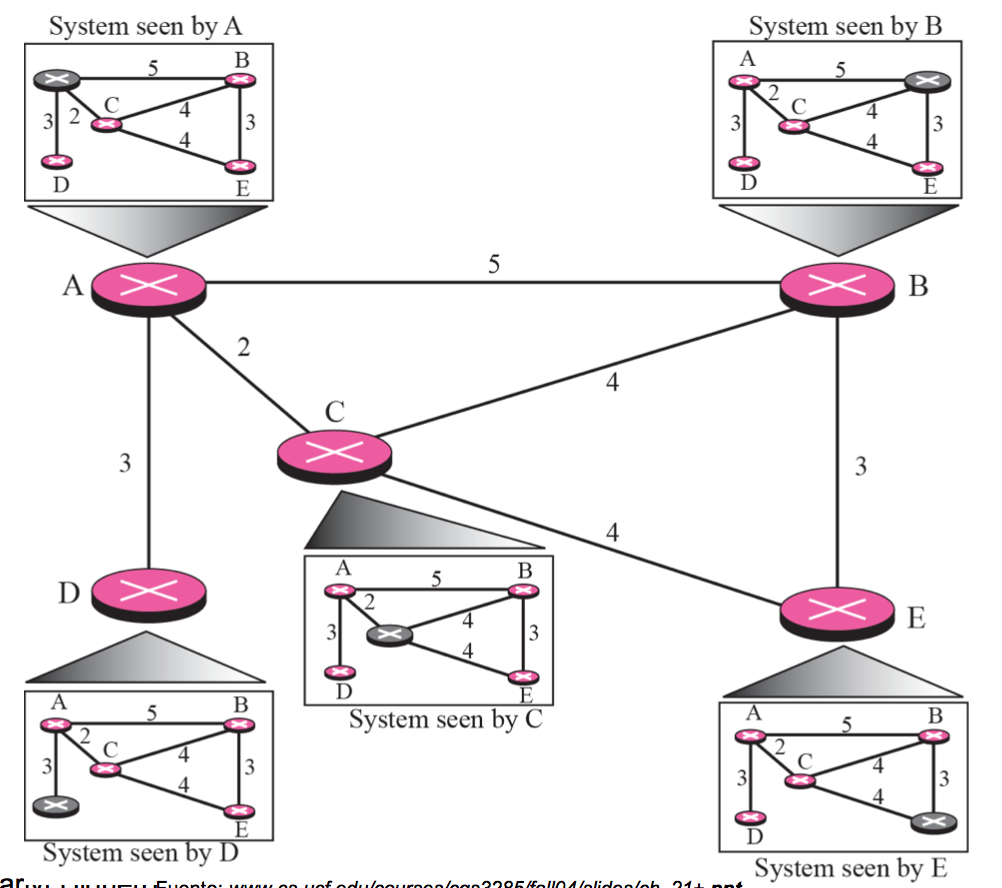
\includegraphics[width=0.3\textwidth]{IGP}
      \caption{Algoritmos Link State}
      \label{fig:Regiones de frecuencias}
  \end{figure}

El \textbf{funcionamiento} de los protocolos Link State, la BD constituye la información que se almacenaría en cada uno de los nodos conteniendo cada entrada:
	
	\begin{itemize}
		\item Identificativo de interfaz (número de enlace).
		\item Información describiendo el estado del enlace (LS): Destino y distancia (métrica)
	\end{itemize}
	
Con esa información cada nodo puede calcular el camino más corto desde él hasta cada nodo. Los cálculos son rápidos.\\

\textbf{¿Cómo logran  la convergencia?} Cada router conoce sus propias redes conectadas directamente. Los routers de estado de enlace intercambian un paquete de saludo para 'conocer' a los routers de estado de enlace conectados directamente. Cada router crea su propio paquete de estado de enlace (LSP) que incluye información sobre los vecinos, como la ID, el tipo de enlace y el ancho de banda. Una vez creado el LSP, el router lo envía a todos sus vecinos que almacenan la información y luego la reenvían hasta que todos los routers tengan la misma información. Cuando todos los routers han recibido los LSP crean un mapa topológico de la red que se utiliza para determinar las mejores rutas para un destino.\\

\textbf{Protocolo de inundación}, para que los encaminamientos puedan adaptarse a las condiciones cambiantes de la red se debe de actualizar la base de datos después de cada cambio en la red. Si dos nodos adyacentes detectan el fallo del enlace actualizarán las entradas correspondientes de la BD construyendo las nuevas TE, transmitirán las nuevas al resto de nodos mediante inundación. Hay que evitar que un mensaje antiguo llegue a corromper la BD, para ello cada mensaje dispone de un número de secuencia o sello de tiempo. \textbf{¿Cómo funciona el mecanismo de inundación?} Se recibe un mensaje y se busca el registro correspondiente en la BD local \footnote{Las actualizaciojnes causan la transmisión del mensaje a través de todas las intefaces excepto por la que llegó el mensaje original}, si el registro existe y el número de la información recibida es mayor que el de la almacenada, actualizar el registro y broadcast del mensaje. Si el registro existe y su número es mayor, transmitir el valor de la BD por la interfaz que llegó el mensaje. Si ambos números son iguales no hacer nada.\\

\textbf{Sincronización de las Bases de Datos} si falla un nodos sólo pueden distribuir información a los vecinos conectados. Cuando termine la inundación existirán dos versiones distintas de la Base de Datos. Este problema, en principio, no tiene importancia. Si las dos mitades separadas mucho tiempo las dos versiones de las BDs evolucionarán independientemente. Establecer conectividad entre dos nodos requiere más que el envío de un registro de la BD, es necesario garantizar la consistencia de las BDs.

Características \textbf{relevantes}:

	\begin{itemize}
		\item Mapa de red actualizado en una base de datos.
		\item Protocolo de inundación para difusión de información
		\item Sincronización de Bases de Datos para alinear las Bases de Datos en los nodos
		\item Algoritmos SPF para cálculos de rutas.
	\end{itemize}
	
\textbf{Conclusiones}:

	\begin{itemize}
		\item Ventajas: Utiliza costes para el cálculo de rutas, convergencia más rápida que protocolos VD y es más escalable soportando división de redes en áreas.
		\item Desventajas: Hace uso de más memorias en los equipos y es más complejo.
	\end{itemize}


\subsubsection{Protocolo OSPF (Open Shortest Path First)}

OSPF es un protocolo de estado del enlace. Viaja sobre IP en las tramas pero requiere mucho procesado y  memoria. En el encendido de la red consume muchos recursos hasta que converge pero luego en estabilidad no consume tanto. Los nodos mantienen un mapa de la red que se actualizará rápidamente ante cualquier cambio. Soporta: BDs distribuidas, procedimiento de inundación, sincronización de las BDs y entradas especiales para rutas externas.\\

Divide la red en \textbf{áreas}. Si el tamaño de una red crece también crecen las BDs, el tiempo de cálculo de las rutas y el volumen de mensajes. En una red grande estos factores pueden ser excesivos. OSPF divide la red en partes independientes interconectadas llamadas áreas unidas mediante un \textbf{área troncal}, cada área se comporta como una red independiente (las BDs sólo contienen info de sus enlaces y mecanismos de inundación hasta la frontera), para poder unir las zonas entre sí algunos routers pertenecen a varias áreas. Se ejecuta sobre IP y tiene tres subprotocolos:

	\begin{itemize}
		\item Protocolo \texttt{Hello}: Comprueba que un enlace está operacional y realiza otras operaciones de control.
		\item Protocolo \texttt{Exange}: Para sincronización inicial de BD.
		\item Protocolo \texttt{Flooding}: Envío de información acerca de actualización de rutas, mantiene sincronizadas las BDs y se utiliza cuando un enlace cambia de estado y en respuesta a una petición.
	\end{itemize}
	
	
\begin{figure}[h]
	\centering
     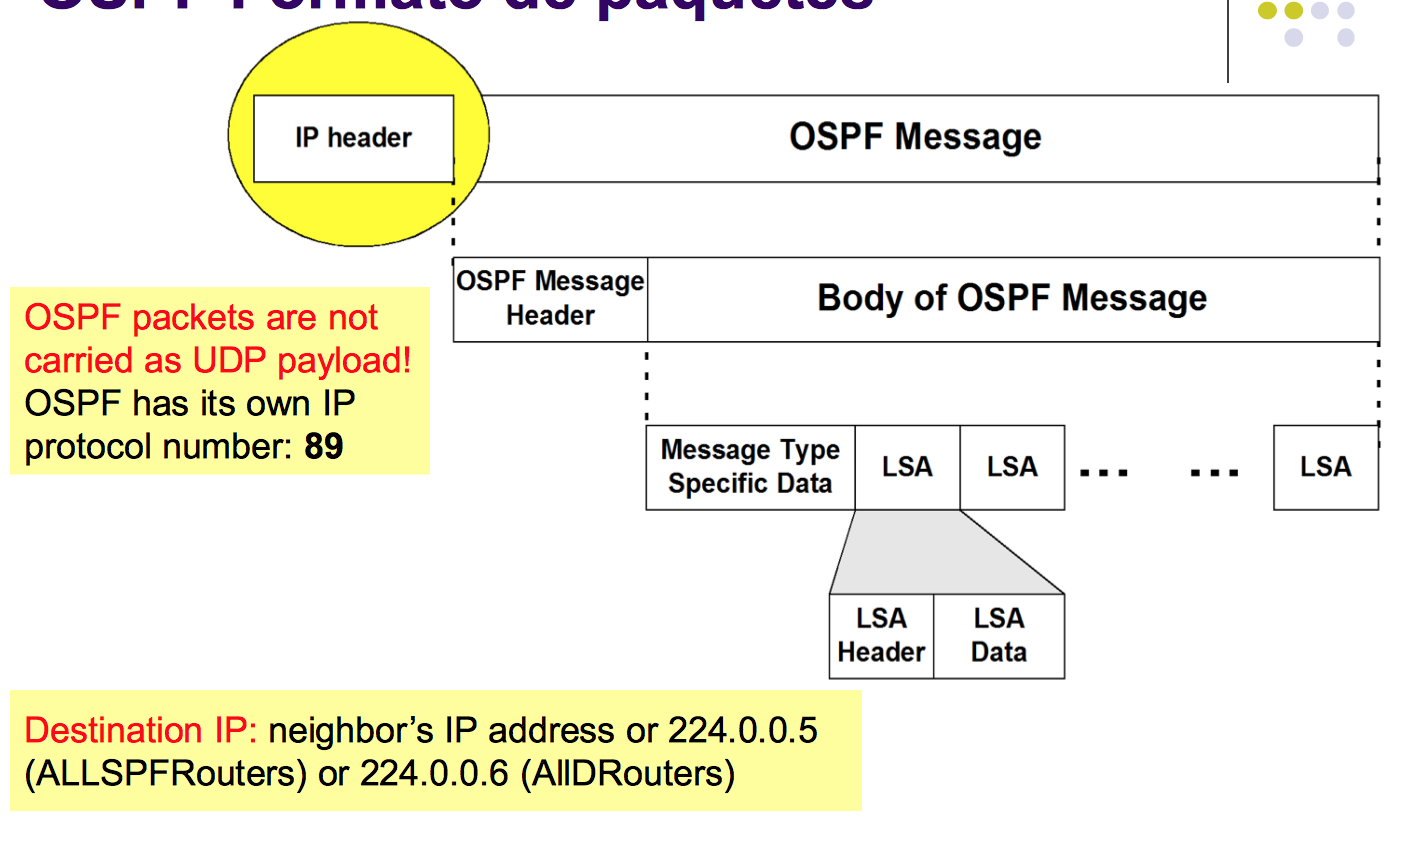
\includegraphics[width=0.4\textwidth]{OSPF}
      \caption{OSPF Formato de Paquetes}
      \label{fig:Regiones de frecuencias}
  \end{figure}
  
\begin{figure}[h]
	\centering
     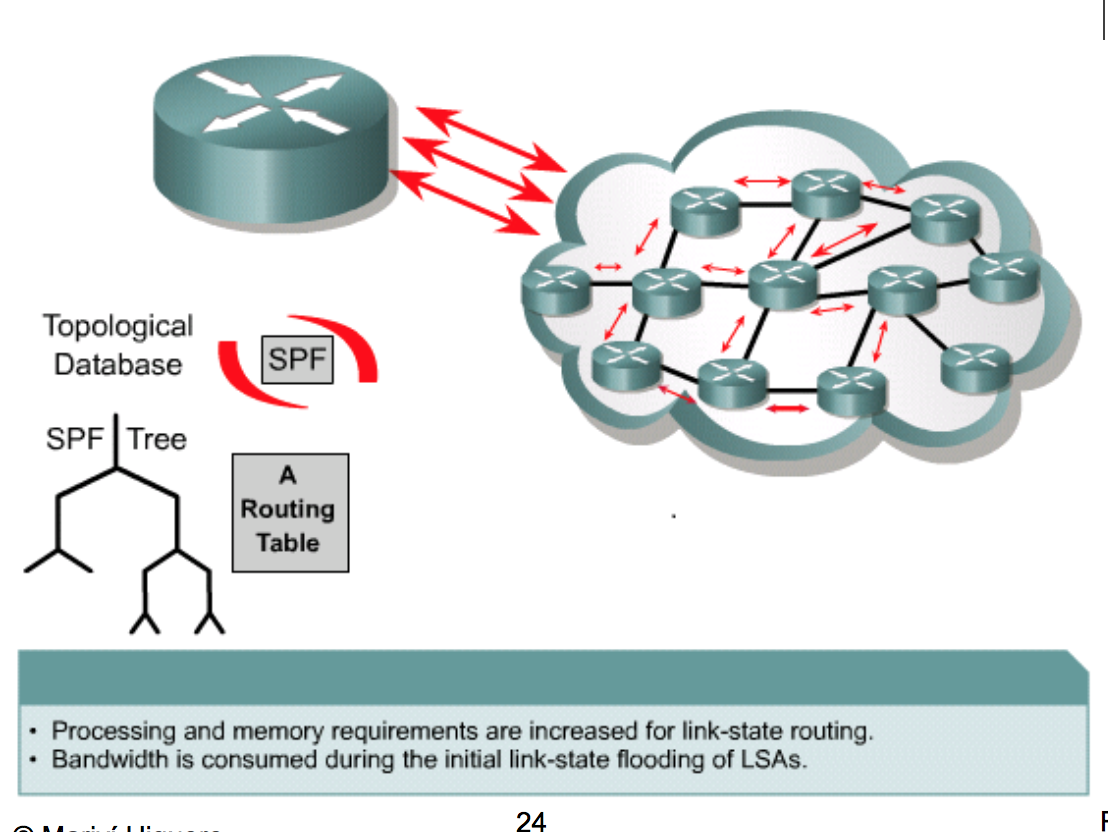
\includegraphics[width=0.4\textwidth]{OSPF2}
      \caption{Protocolo OSPF}
      \label{fig:Regiones de frecuencias}
  \end{figure}
	
\textbf{OSPF vs RIP}:

	\begin{itemize}
		\item OSPF es mucho más complejo que RIP, la gestión requiere una mayor cantidad de información, las implementaciones requieren más código y son más complejas
		\item Requerimientos mayores de los protocolos LS, utilizan más memoria, requieren más CPU y requieren mucho ancho de banda en el startup inicial.
		\item OSPF es más eficiente y utiliza menos mensajes pero es más complejo que RIP.
		\item Distance Vector Routing, cada nodo conoce a sus vecinos directamente conectados, cada nodo sólo conoce distancias a destinos, cada nodo envía periódicamente su tabla de encaminamiento a sus vecinos \footnote{Los updates pueden ser grandes pero sólo viajan por un enlace}. Si todos los nodos envían los updates de sus TE, las tablas de encaminamiento terminan convergiendo.
		\item Lisnk State Routing, cada nodo conoce la distancia a sus vecinos, cada nodo conoce la topología entera. La información de enlaces y distancias se envía a todos los nodos de la ted. Cada nodo calcula las TE de forma independiente.
	\end{itemize}
	
\subsection{Encaminamiento en Internet}

\subsubsection{Protocolos EGP}

\textbf{BGP} (\textbf{Border Gateway Protocol}) es el estándar de facto. Proporciona a cada AS capacidad para:

	\begin{enumerate}
		\item Obtener información de alcanzabilidad de los ASs vecinos.
		\item Propagar la información de alcanzabilidad desde los ASs vecinos.
		\item Determinar rutas 'buenas' a destinos basadas en información de alcanzabilidad y políticas de encaminamiento.
	\end{enumerate}
	
Permite a las subredes anunciar su existencia al resto de Internet. \textbf{Características} de BGP:

	\begin{itemize}
		\item Limitaciones de los protocolos de vector distancia: Toda la información de la ruta se concentra en la métrica y no siempre la ruta más corta es la preferida, es insuficiente para la resolución de bucles.
		\item Si se utilizara un protocolo más potente del estado del enlace puede que no todos los equipos tengan las mismas preferencias. Las técnicas para evitar bucles podrían suponer grandes overheads. Los broadcasts y cálculos de la BD a todo Internet demasiado grandes.
	\end{itemize}

\textbf{Estrategia de rutado} de BGP. \textbf{Path Vector Routing}, toda la información de actualización de encaminamiento llevará la lista completa de SAs recorridos. Se daría un bucle si un AS estuviera listado 2 veces. La protección contra bucles es simple: cuando un SA reciba un anuncio de ruta, el router exterior comprobará que su SA no esté en la lista: si el SA está en la lista el router rechaza emplear esa ruta y si no aparece añadirá su identificativo antes de seguir transmitiendo el anuncio. Ventajas: no requiere que todos los routers utilicen las mismas métricas y si se actualizan los path vector de forma adecuada se asegura que se evitan los bucles.
  
\begin{figure}[h]
	\centering
     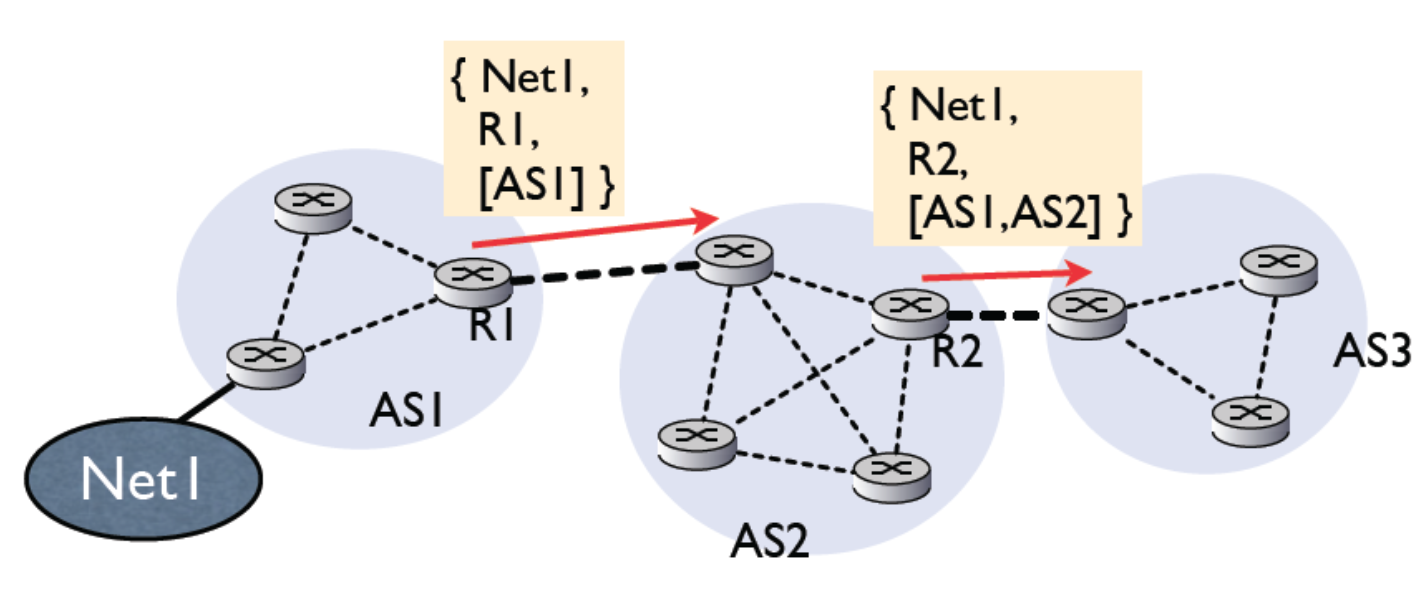
\includegraphics[width=0.4\textwidth]{PathVector}
      \caption{Path Vector}
      \label{fig:Regiones de frecuencias}
  \end{figure}
	
\textbf{Atributos de las rutas}, las rutas se describen mediante un conjunto de atributos, de los cuales los más importantes son: lista de SAs atravesados y lista de redes accesibles. Cuando hay varias rutas disponibles se añaden atributos para facilitar la elección. Formato de los atributos, tripleta de longitud variable:

	\begin{verbatim}
	<attribute type, attribute length, attribute value>
	\end{verbatim}

\begin{figure}[h]
	\centering
     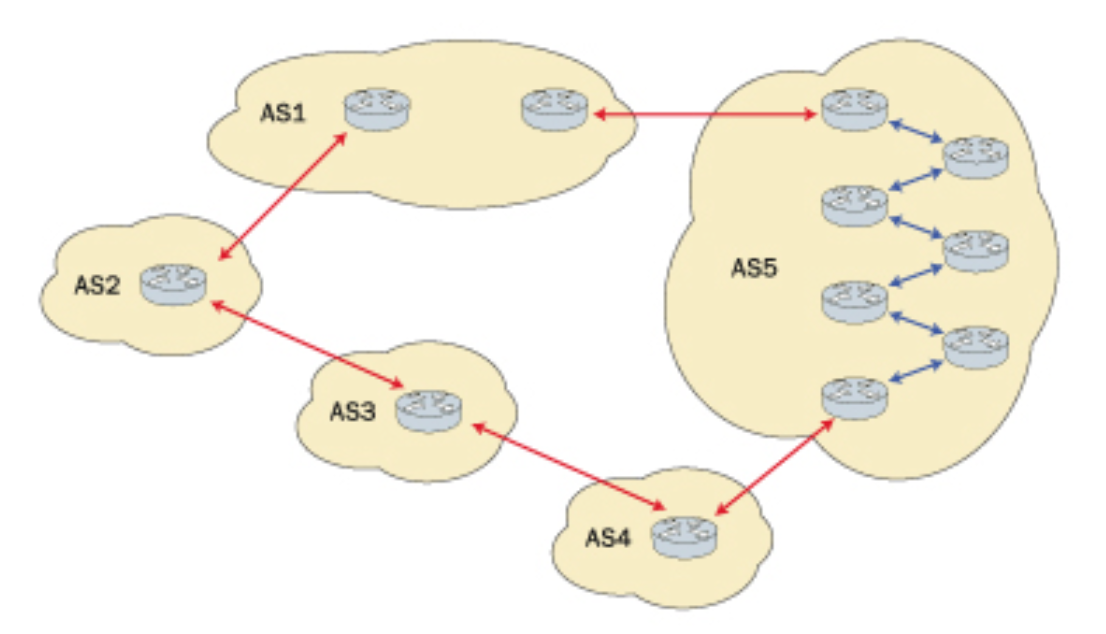
\includegraphics[width=0.4\textwidth]{Rutas}
      \caption{Atributos de las Rutas}
      \label{fig:Regiones de frecuencias}
  \end{figure}

\textbf{Funcionamiento de BGP sobre TCP}, decisión clave sobre el diseño. Como \textbf{ventajas} delega funciones de control en TCP y el protocolo es mucho más simple: no se requiere diseñar mecanismos de recuperaciones de errores, no hay necesidad de adecuar el tamaño de los paquetes BGP al tamaño de los datagramas y no hay necesidad de temporizadores para comprobar que el paquete llega a su destino. Las transferencias de información son fiables, se pueden utilizar transferencias incrementales en lugar de transmitir todo el contenido de las tablas salvo la fase inicial.\\

\textbf{Sincronización con los IGPs}:

	\begin{itemize}
		\item \textbf{Mediante BGP los border routers}: Aprenden rutas de sus ASs vecinos y seleccionan rutaas para los destinos remotos: se sincronizan a través de conexiones internas y deben sincronizar sus actualizaciones con modificaciones en las tablas de encaminamiento locales.
		\item Mediante el IGP los border routers de un AS anuncian rutas externas y aprenden conectividad interna.
		\item BGP y el IGP deben mantenerse consistentes para proporcionar encaminamientos estables.
	\end{itemize}
	
\hrulefill
	
\clearpage


\begin{framed}
	\begin{center}
    	\Large{\underline{Redes de Transporte}} \\
    	\scriptsize{3º Ingeniería de Telecomunicaciones | UPV/EHU}\\
     	%Actualizado por última vez el \today \\
     	"\textsl{Under-promise and over-deliver}." \\
     	%\hspace{5 pt} \\
     	\small{\textbf{Javier de Martín -- 2016}}
	\end{center}
\end{framed}
	
\section{\underline{Transmisión}}

\subsection{Introducción}

\subsubsection{Introducción a las redes de transmisión}

La \textbf{transmisión} es la función de transporte de información de un punto a otro, está presente en la red de acceso \footnote{La mayor parte de la red es para transmitir, no para conmutar} y de transporte \footnote{Interconecta los nodos de conmutación}. Los objetivos son la transparencia para el soporte de todo tipo de señales, uso eficaz de los recursos (multiplexación), adaptación a los medios de transmisión y gestión, operación y mantenimientos óptimos.\\




La red de transporte es el soporte de transmisión para toda la gana de servicios de las redes de conmutación.

\begin{figure}[h]
	\centering
     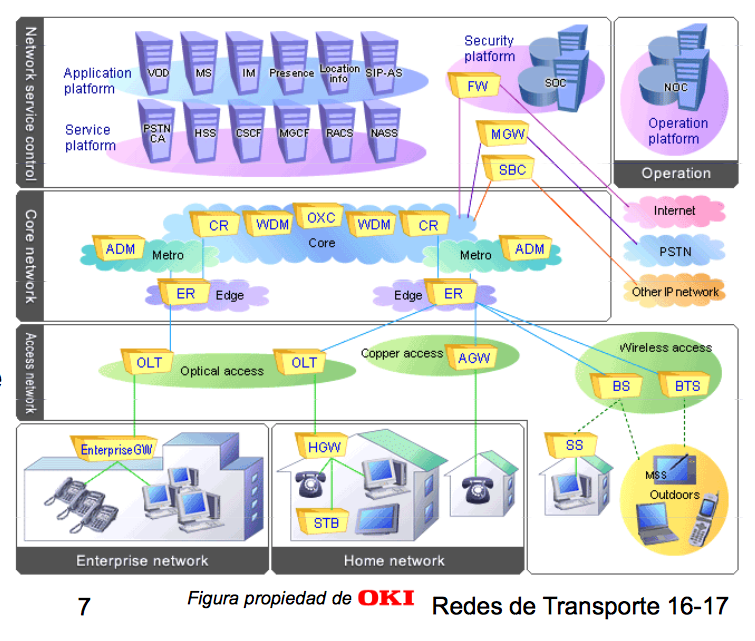
\includegraphics[width=0.35\textwidth]{NGN}
      \caption{NGN}
      \label{fig:Regiones de frecuencias}
  \end{figure}

En las NGN la Red de Acceso es fundamentalmente óptica, en el núcleo de red se encuentra la Red de Transporte y redes específicas (nodos de servicio).\\

\textbf{Elementos} en la red de transporte (TX):

	\begin{itemize}
	\item Medios de transmisión : Fibra óptica (redes ópticas en la red de transporte)
	\item Equipos/Funciones de transmisión: Multiplexación, Inserción/Extracción, Transconexión y Amplificación.
	\end{itemize}
	
La \textbf{evolución de las Redes de Transoprte} consiste en adaptarse a las características de tráfico. Hoy en día las sesiones son más largas, el tráfico es impredecible, mayor cantidad de datos... Aparecen las \textbf{redes multiservicio}:

	\begin{equation*}
	\text{PDH} \rightarrow \text{SDH} \rightarrow \text{NG-SDH} \rightarrow \text{OTN/WDM} \rightarrow \text{MPLS-TP}
	\end{equation*}
	
y en las redes de datos EoT (Ethernet on Transport).

\begin{figure}[h]
	\centering
     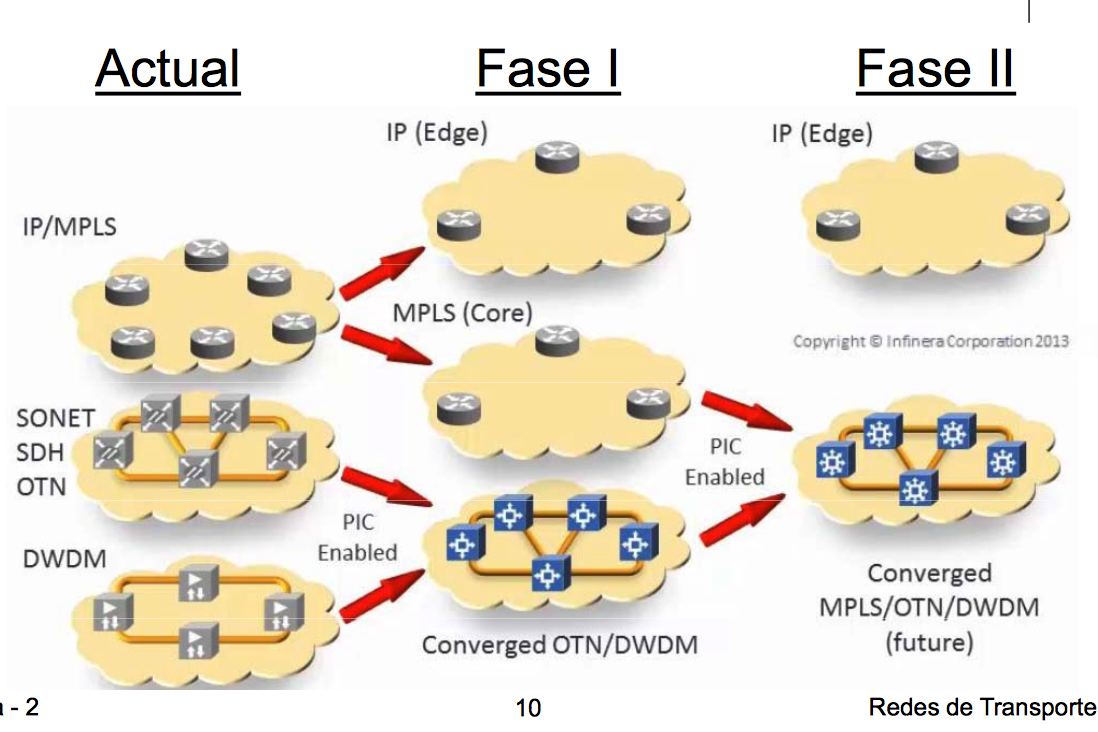
\includegraphics[width=0.35\textwidth]{EvolucionRdT}
      \caption{Evolución de las Redes de Transporte}
      \label{fig:Regiones de frecuencias}
  \end{figure}

\subsection{Transmisión en Redes Multiservicio}

Una característica de una red óptica de transporte es su \textbf{oferta de transporte para cualquier señal cliente}, con independencia de los aspectos específicos del cliente, eso es, las funciones de una red óptica de transporte pueden ser independientes de la información característica de las señales cliente.

%\begin{figure}[h]
%	\centering
%     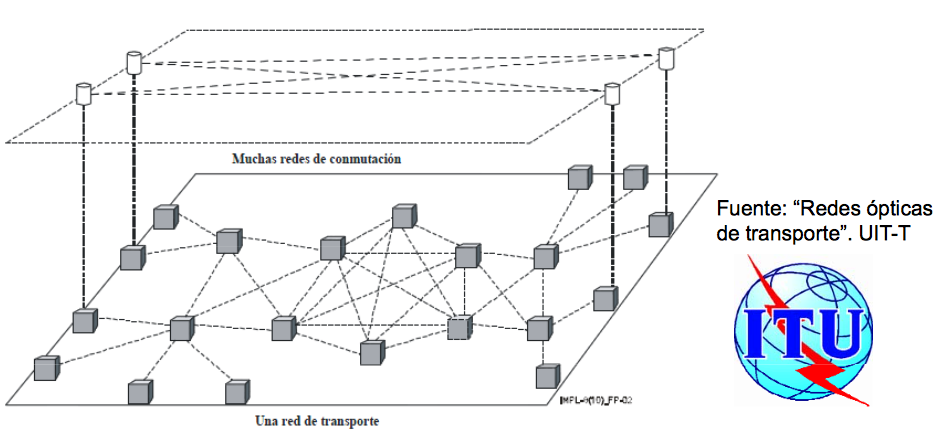
\includegraphics[width=0.35\textwidth]{RdT}
%      \caption{Redes Ópticas de Transporte}
%      \label{fig:Regiones de frecuencias}
%  \end{figure}

 \textbf{Capas de las Redes de Transporte ópticas}\\
  
\begin{itemize}
\item La \textbf{capa cliente (datos)} (figura \ref{fig:capasTransporte}) procesa los datos en el campo eléctrico y se aplica a través de un equipo que cumple las funciones de multiplexación de señal, encaminamiento, supervisión, control del funcionamiento, vigilancia y supervivencia de la red. Incorpora diversos servicios de baja velocidad de voz, datos y líneas privadas.

\begin{figure}[h!]
	\centering
     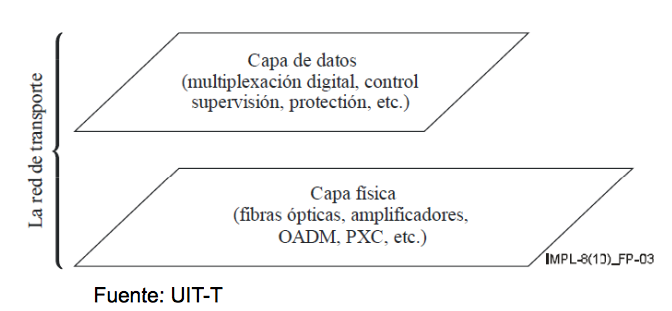
\includegraphics[width=0.35\textwidth]{Capa}
      \caption{Capas de la Red de Transporte}
      \label{fig:capasTransporte}
  \end{figure}
  
\item  La \textbf{capa óptica} proporciona trayectos de luz a la capa cliente siendo los trayectos de luz los enlaces físicos entre los elementos de la red de la capa cliente.
\end{itemize}  
 
\textbf{Características de una red óptica de transporte}, la capa cliente (datos) de una red óptica se caracteriza por su arquitectura de red, jerarquía de multiplexación, técnica de supervisión, técnica de sincronización de la red y procedimientos de supervivencia de la red. 

\begin{itemize}
\item \textbf{Redes públicas (multiservicio)}: 
	\begin{itemize}
	\item \begin{itemize}
	\item \textbf{PDH (Plesiochronous Digital Hierarchy)}: Ha sido muy utilizada en las redes públicas de telecomunicaciones, pero puede considerarse obsoleta para redes de transporte.
	\item \textbf{SDH (Synchronous Digital Hierarchy)}: Ha prevalecido en las infraestructuras públicas de transporte. SDH ofrece una multiplexación por división en el tiempo eficiente para señales de baja velocidad y permite que estas señales se transporten en la re de manera fiable y bien gestionada.
	\item \textbf{OTN (Optical Transport Network)}: Se está convirtiendo en la actual jerarquía de multiplexación predominante que se utiliza ahora con los clientes que disponen de anchos de banda de servicio variables.
	\end{itemize}
	\end{itemize}
	\item \textbf{Redes privadas (datos)}: 
		\begin{itemize}
		\item \textbf{Ethernet}: Es una tecnología de red por paquetes. Utilizada en el ámbito de las empresas y para el transporte entre proveedores y servicios.
		\item \textbf{MPLS  (Multiprotocol Label Switching)}: Diseñado para unificar el servicio de transporte de datos para las redes basadas en circuitos y las basadas en paquetes.
		\end{itemize}
\end{itemize}
 
%\begin{figure}[ht]
%	\centering
%     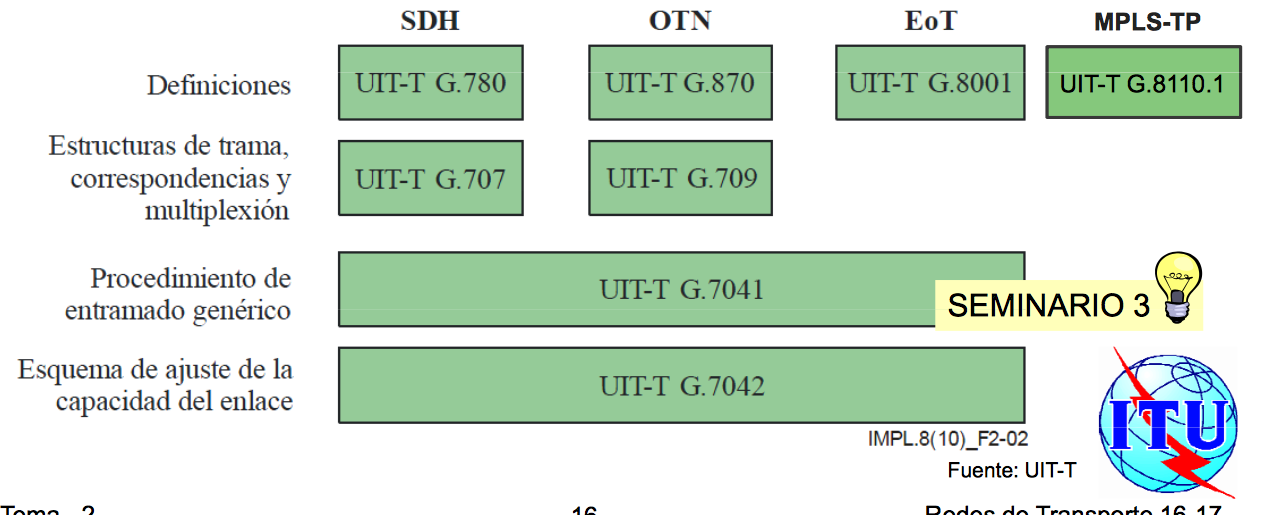
\includegraphics[width=0.35\textwidth]{Recomendaciones}
%      \caption{Recomendaciones de redes ópticas de Transporte}
%      \label{fig:Regiones de frecuencias}
%  \end{figure}
 

\subsubsection{Jerarquías Digitales de Multiplexación TDM}

PDH obsoleta en redes de transporte y SDH muy implantada y emergente en su versión NG-SDH.\\

%\begin{figure}[ht]
%	\centering
%     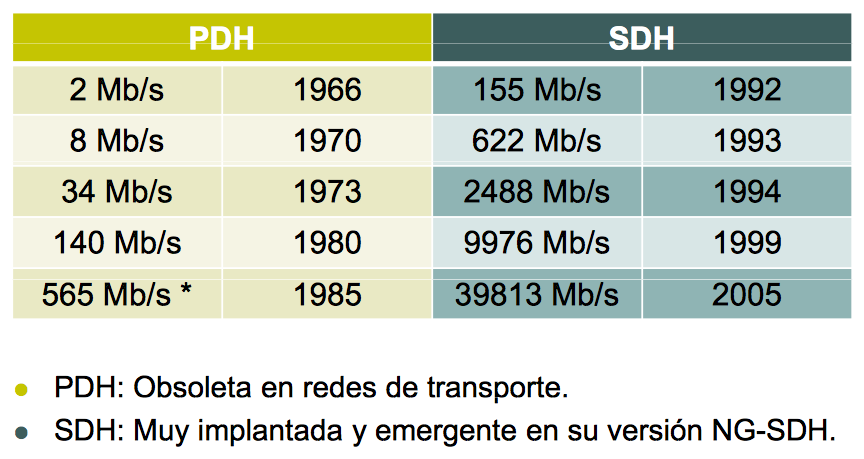
\includegraphics[width=0.35\textwidth]{PDHSDH}
%      \caption{Secuencia Histórica de PDH y SDH}
%      \label{fig:Regiones de frecuencias}
%  \end{figure}
  
En \textbf{SDH} los multiplexores tienen un reloj independiente de las otras fuentes, en \textbf{SDH} hay una única señal de reloj para todos los equipos. Los 2Mb/s de PDH es la base como señal para la multiplexación, proviene de los MIC PCM. El último estándar es la señal de 140Mb/s.\\

\textbf{PDH/JDP: Jeraraquía Digital Plesiócrona}:

	\begin{itemize}
	\item El \textbf{plan de multiplexación MDT (TDM)} recomendado por la UIT-T para la multiplexación de señales plesiócronas basado en la banda base de 2Mbits/seg (origen de la señal MIC).
	\item  \textbf{Plesiócrono} indica que las frecuencias de reloj de los distintos niveles no están sincronizadas entre sí, los relojes son casi-síncronos. 
	\item El reloj del multiplexor es \textbf{independiente} de los relojes de las señales tributarias de orden inferior. 
	\item La multiplexación se realiza \textbf{bit a bit}, eso es posible ya que todos los canales han sido digitalizados y multiplexados por el mismo dispositivo MIC.
	\end{itemize}



\subsubsection{Características de PDH}

Las multiplexaciones (figura \ref{fig:Multiplex}) se realizan agrupando \textbf{cuatro afluentes} o \textbf{tributarios} de orden inferior para obtener un flujo de velocidad binaria superior, la \textbf{señal multiplex}.

\begin{figure}[ht]
	\centering
     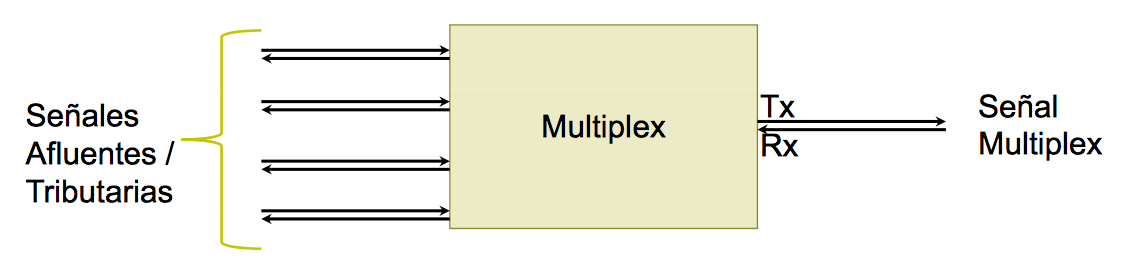
\includegraphics[width=0.35\textwidth]{Multiplex}
      \caption{Señal Multiplex}
      \label{fig:Multiplex}
  \end{figure}

El equipo Multiplex multiplexa y demultiplexa las señales en TDM. 
  
 \begin{figure}[ht]
	\centering
     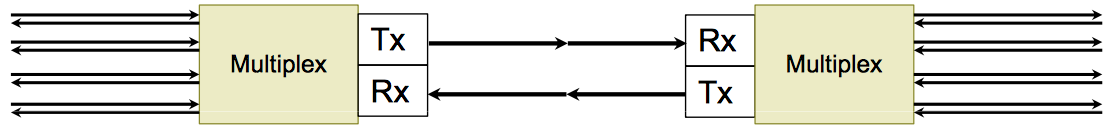
\includegraphics[width=0.35\textwidth]{SdT}
      \caption{Sistema de Transmisión (2 equipos MUX)}
      \label{fig:Regiones de frecuencias}
  \end{figure}
  
  \begin{itemize}
  \item Para las velocidades de 2, 8, 34 y 140 Mbps la UIT-T recomienda interfaces normalizados y que la interconexión se haga por medio de repartidores.
  \item  Para las velocidades de 565 Mbs/seg no se ha normalizado ningún interfaz. En el caso del equipo multiplex se conecta directamente al ETL (Equipo Terminal de Línea). 
  \item La multiplexación en todos los casos se realiza bit a bit.
  \item Se utilizan técnicas de relleno o justificación, por eso al juntar 4 señales afluentes no se obtiene la multiplicación por 4 en la señal multiplex, se añaden bits extra.\\
  \end{itemize}

\textbf{Características de los múltiplex}: 

\begin{itemize}
\item Multiplexan afluentes plesiócronos por le método de justificación positiva.
\item  Se dice que dos señales son plesiócronas entre sí cuando tienen una velocidad parecida, aunque no exactamente igual.\footnote{En una interfaz de 2Mbps (2.048 Kbits/s tienen una tolerancia de $\pm$ 50 ppm, esto es, cada afluente puede tener una velocidad comprendida entre 2047898 y 2048102 bits/seg)}.
\end{itemize}



\begin{figure}[h]
	\centering
     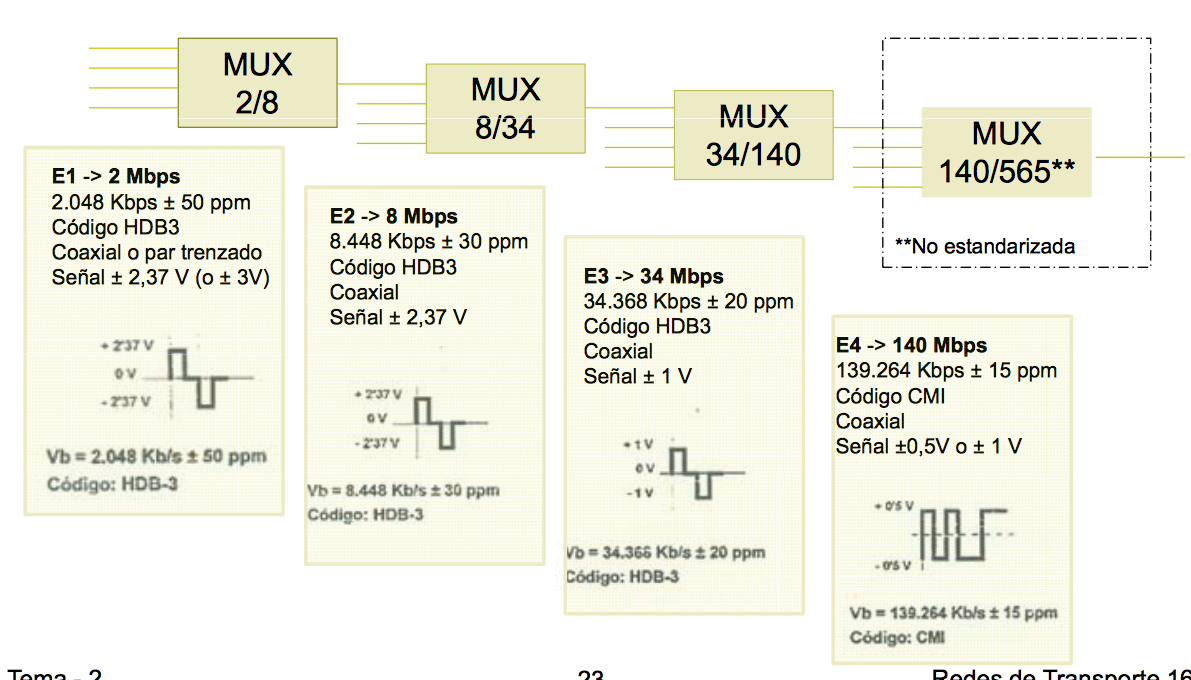
\includegraphics[width=0.35\textwidth]{CaracPDH}
      \caption{Características PDH}
      \label{fig:Regiones de frecuencias}
  \end{figure}
  
\subsubsection{Interconexión de Equipos}

\begin{figure}[!ht]
	\centering
     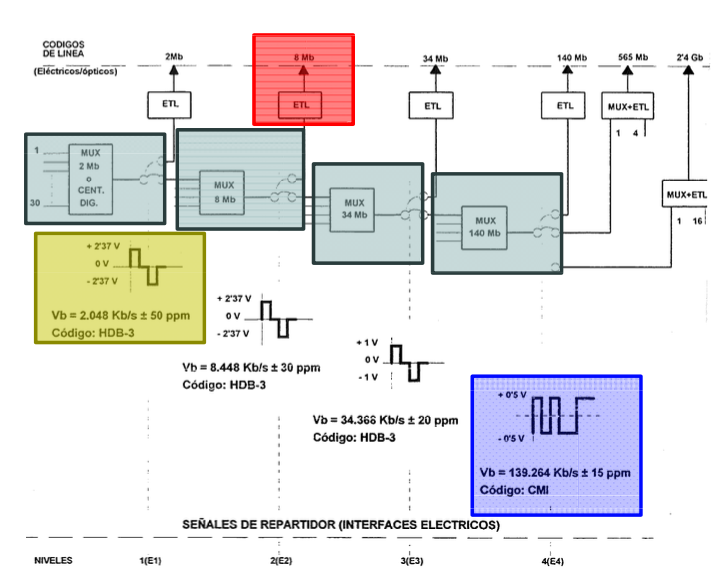
\includegraphics[width=0.35\textwidth]{ETL}
      \caption{Uso de repartidores y ETL hacia la línea}
      \label{fig:Regiones de frecuencias}
  \end{figure}

El ETL se utiliza para adaptar la señal del múltiplex para ser transmitida.

%\begin{figure}[!ht]
%	\centering
%     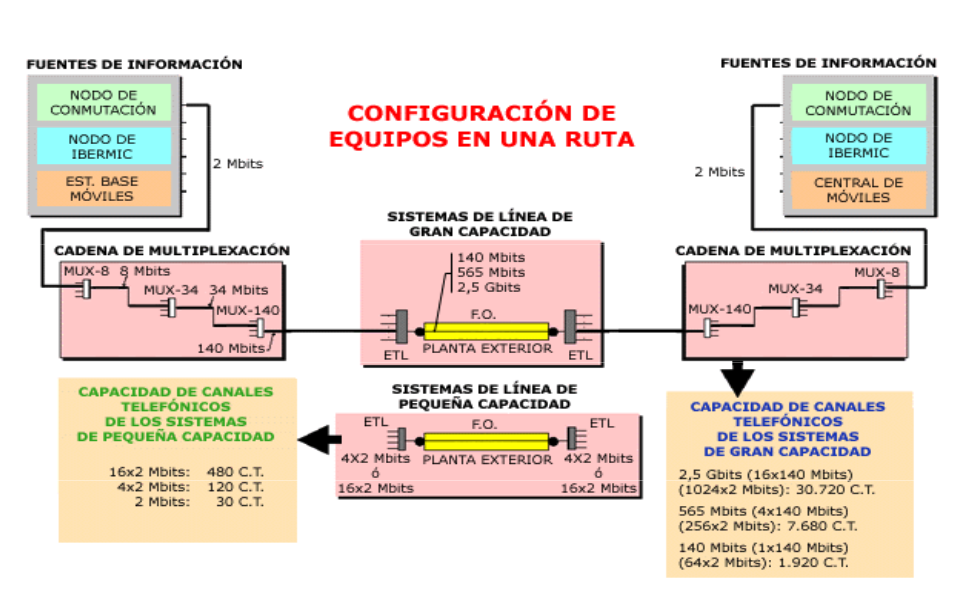
\includegraphics[width=0.35\textwidth]{Intercx}
%      \caption{Interconexión de equipos}
%      \label{fig:Regiones de frecuencias}
%  \end{figure}

La entrada a la cadena de multiplexación permite la entrada de diferentes tipos de señales a pesar de haber sido diseñado originalmente para señales telefónicas.

\subsubsection{Jerarquía Digital PDH}

\begin{figure}[!ht]
	\centering
     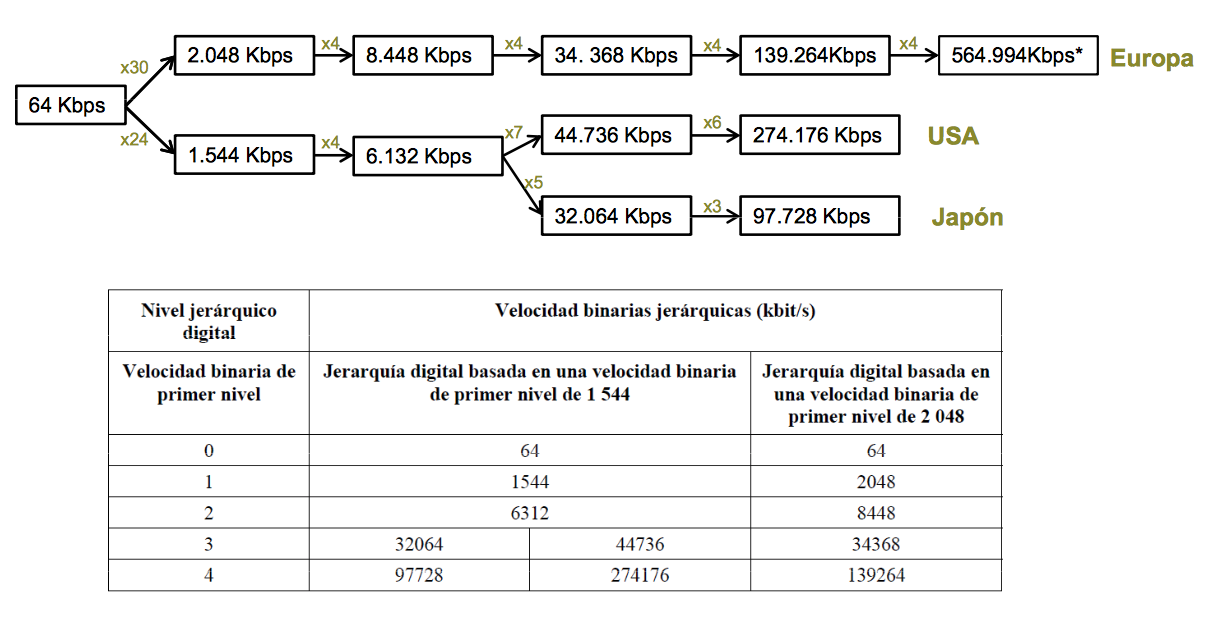
\includegraphics[width=0.35\textwidth]{Jerarquia}
      \caption{Jerarquía Digital PDH}
      \label{fig:Regiones de frecuencias}
  \end{figure}
  
La jerarquía digital PDH tiene varios problemas, entre ellos que para extraer una señal de 2Mb no se puede hacer directamente, hay que demultiplexar toda la señal y no es compatible entre países.\\

\subsubsection{MUX MDT de Afluentes}

\begin{itemize}
\item Los equipos PDH no están sincronizados con un único reloj. Se sincronizan con diferentes relojes a la misma velocidad pero con tolerancias.
\item Problema de la multiplexación MDT: Es necesario que los cuatro afluentes tengan exactamente la misma velocidad binaria, y que la velocidad de la señal múltiplex sea exactamente cuatro veces mayor que la de cada afluente.
\end{itemize}

Se plantea el siguiente problema:

\begin{figure}[!ht]
	\centering
     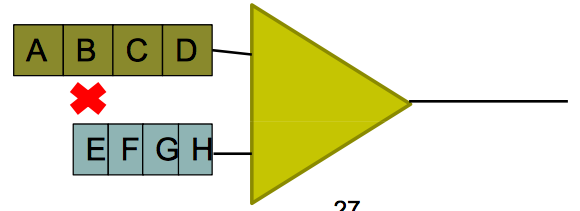
\includegraphics[width=0.35\textwidth]{Problemas}
      \caption{Multiplexación MDT de Afluentes}
      \label{fig:Regiones de frecuencias}
  \end{figure}
  

Solución a la multiplexación MDT de afluentes sincronizados:

	\begin{itemize}
	\item Multiplexación de afluentes plesiócronos con justificación positiva (o negativa).
	\item Previo a realizar la multiplexación MDT (TDM) se sincronizan los cuatro afluentes utilizando los métodos de justificación.
	\item La velocidad de los afluentes sincronizados es exactamente $1/4$ parte de la velocidad de la señal múltiplex.
	\item La justificación consiste en la variación de forma controlada de la velocidad de la velocidad binaria del afluente, de forma que se adapte a una velocidad binaria distina de la suya propia sin pérdida de información.
	\end{itemize}

%\subsubsection{Multiplexación MDT entre Países}

La \textbf{justificación positiva}:

	\begin{itemize}
		\item Consiste en la variación de forma controlada de la velocidad binaria e una señal digital, de forma que se adapte a una velocidad binaria distinta de la suya propia, sin pérdida de información.
	\end{itemize}



\textbf{Sincronización de Afluentes}. Los tres bits que aparecen al inicio de cada afluente son fijos. La longitud de cada afluente varía, $50b + 52b + 52b + 51b \pm S = 205/6b$ dependiendo de si el bit S (bit de justificación) es de información o relleno.\\

\begin{figure}[!ht]
	\centering
     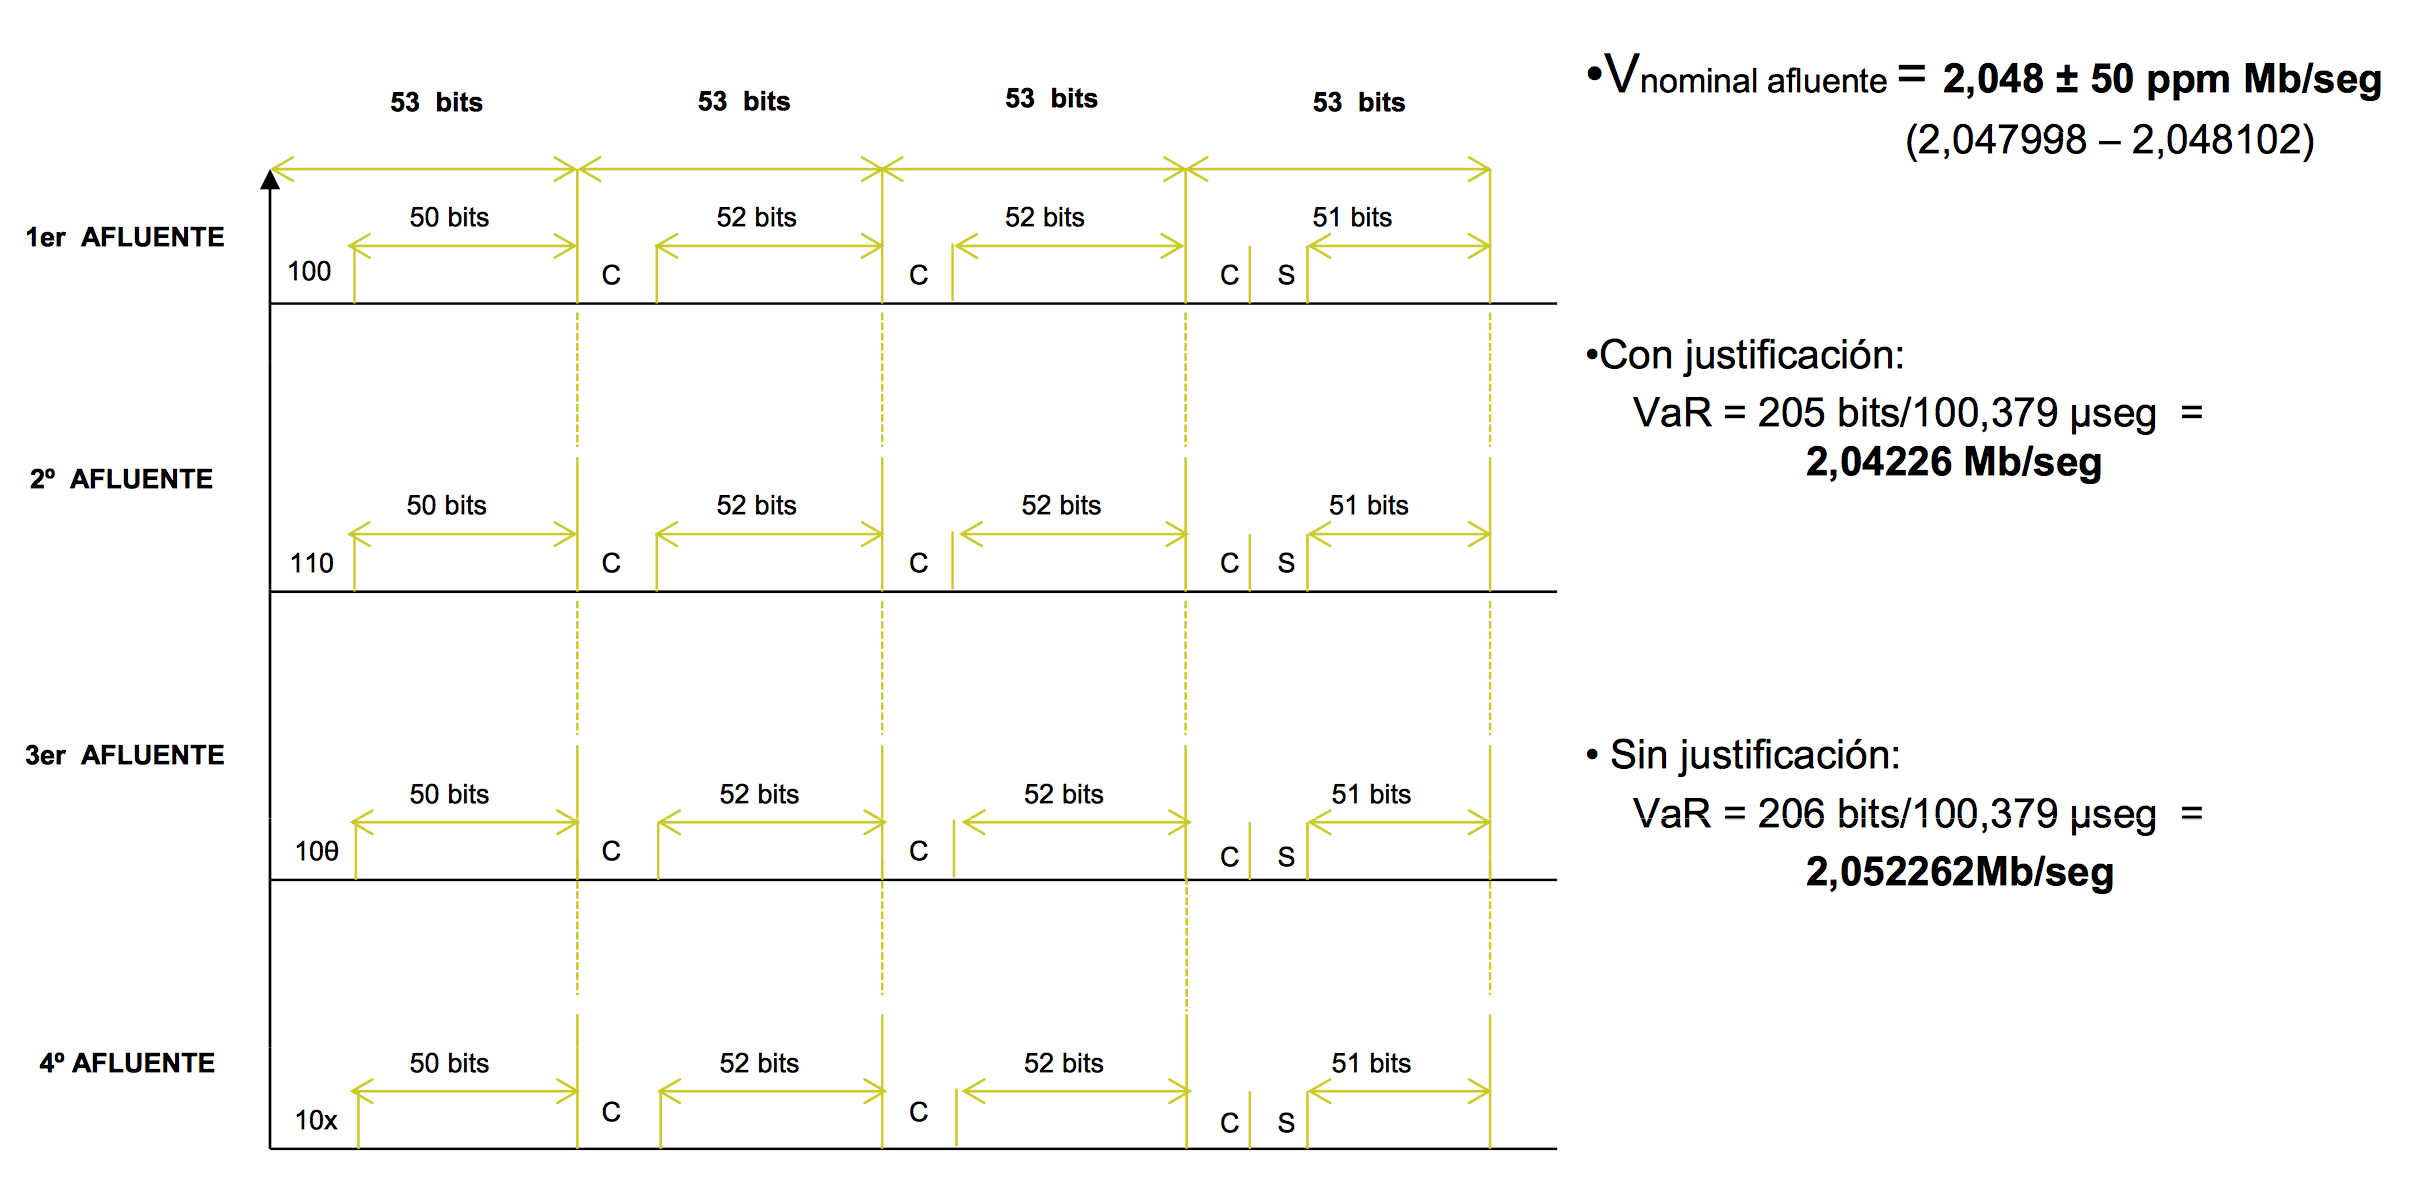
\includegraphics[width=0.5\textwidth]{sync}
      \caption{Sincronización de Afluentes de 2.112 kb/seg}
      \label{fig:Regiones de frecuencias}
  \end{figure}
  
\begin{itemize}
\item \textbf{Bits de oportunidad de justificación (S)} pueden llevar información del afluente o ser de relleno. 
\item \textbf{Bits de control de justificación (C)}, \texttt{111} es justificación positiva y el bit S debe de ser ignorado o \texttt{000} indica que hay ausencia de justificación y el bit S es información del afluente.
\item En \textbf{ausencia de justificación} se lee más deprisa de lo que se escribe (2.052,22 kbps > 2.048 kbps).
\item En \textbf{presencia de justificación} se lee más despacio de lo que se escribe (2.042,26 kbps < 2.048 kbps). 
\item Con velocidad nominal, la tasa de justificación será de 42,42\%.
\end{itemize}
  


\begin{figure}[!ht]
	\centering
     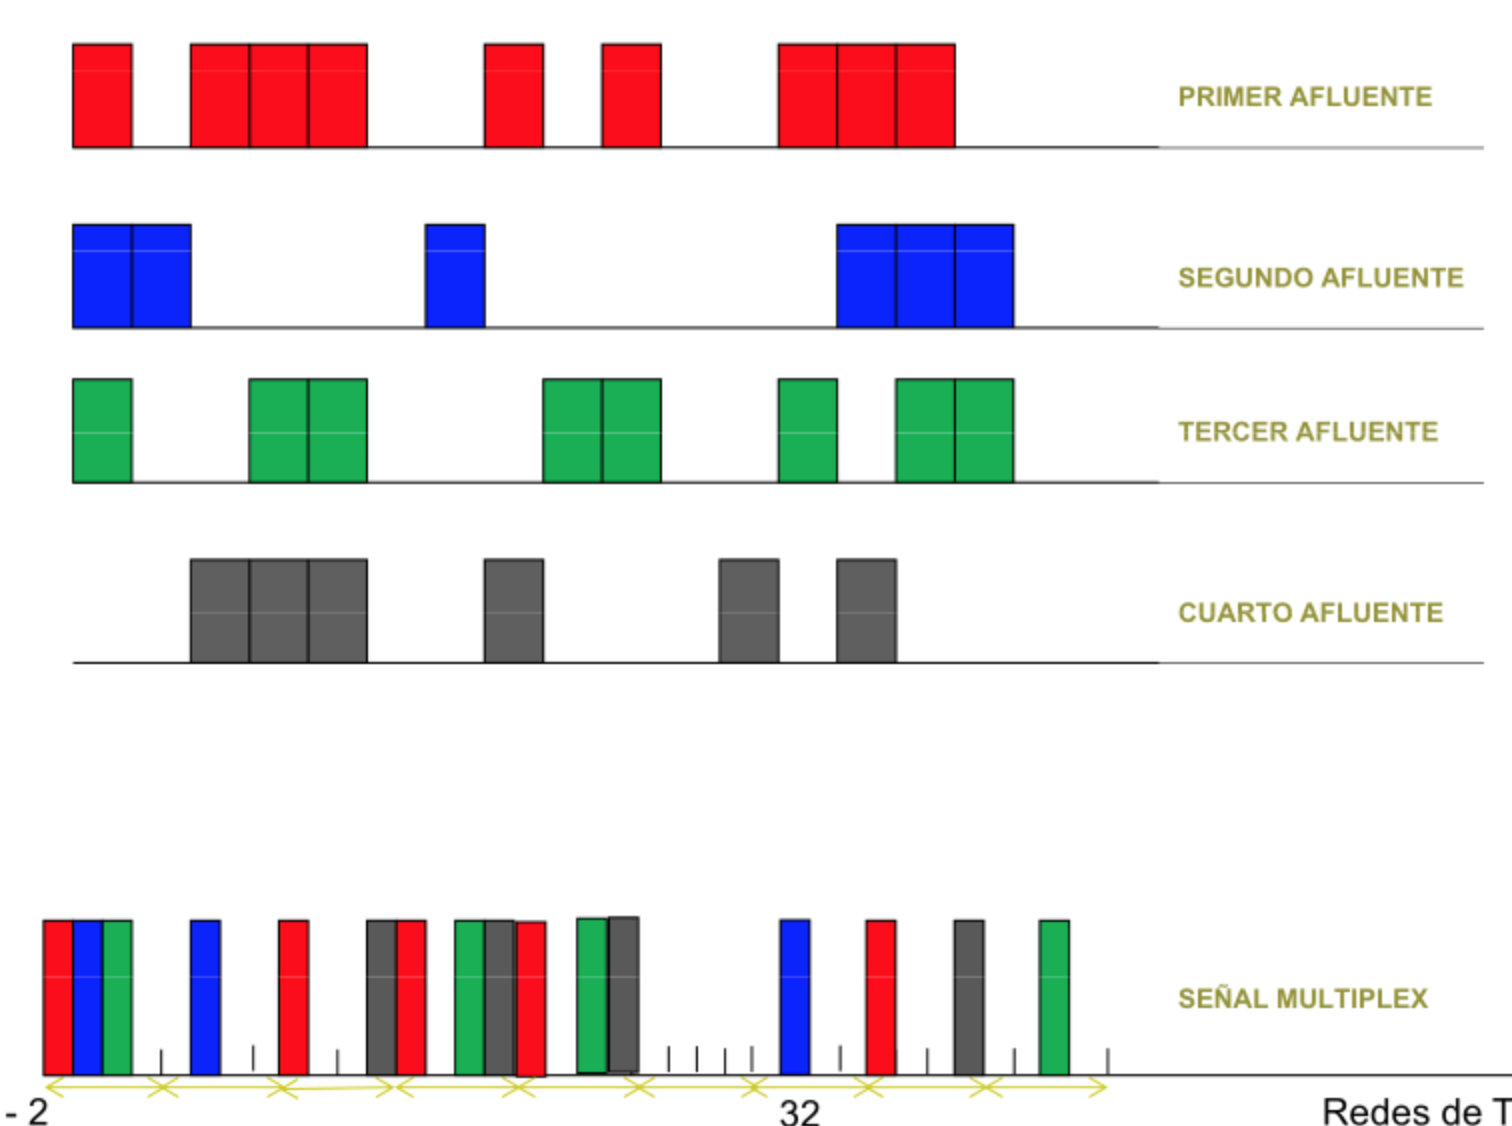
\includegraphics[width=0.35\textwidth]{MDT}
      \caption{Multiplexación MDT bit a bit}
      \label{fig:Regiones de frecuencias}
  \end{figure}
  
Las \textbf{memorias elásticas} 

\begin{itemize}
\item En transmisión permiten la sincronización de los afluentes plesiócronos.

\begin{figure}[!ht]
	\centering
     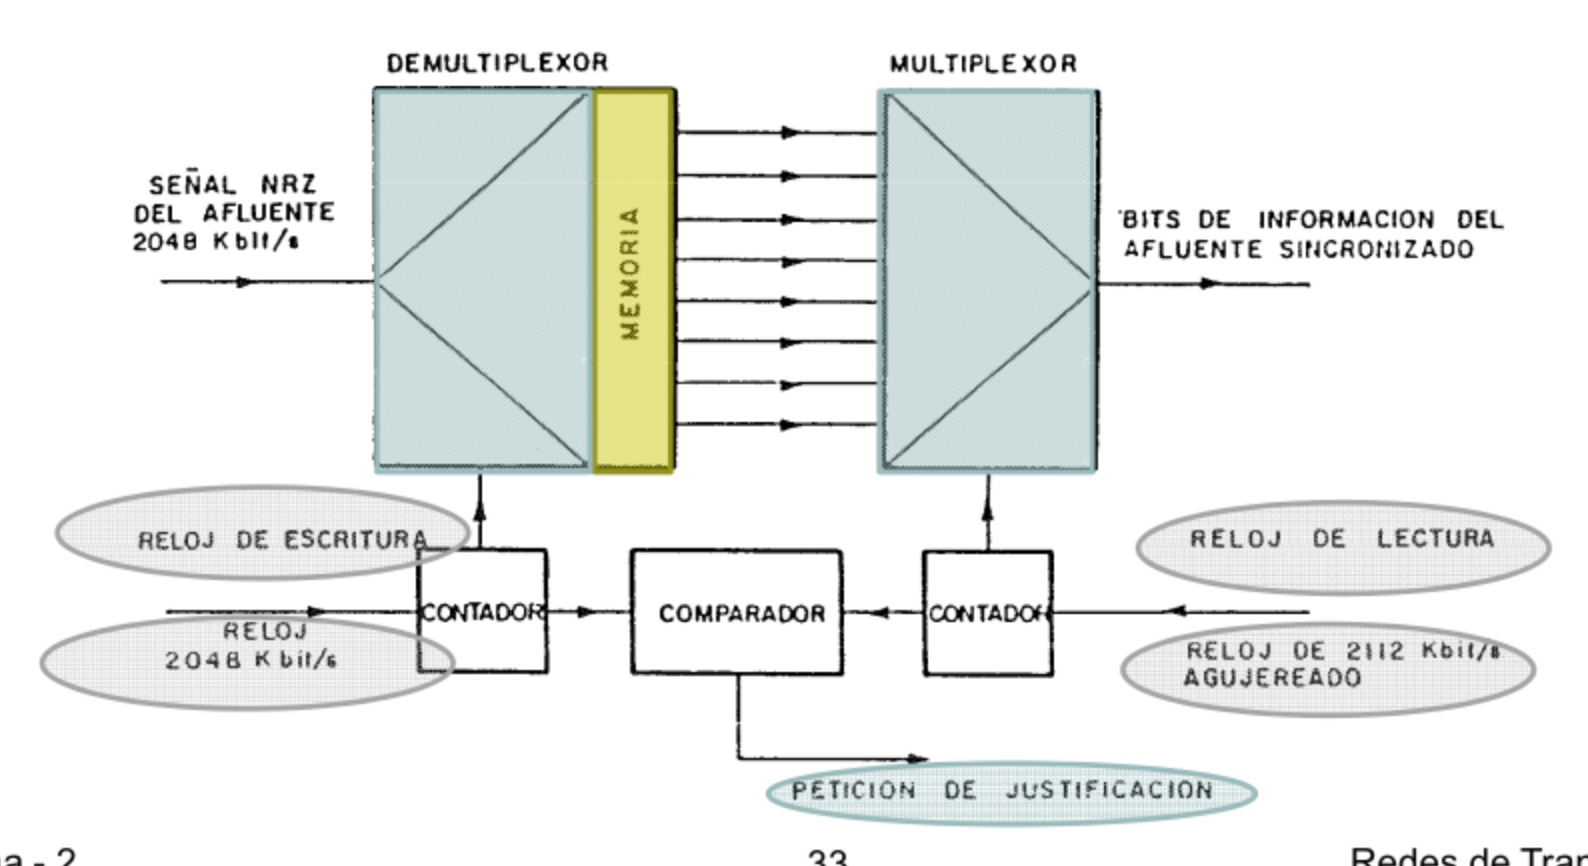
\includegraphics[width=0.5\textwidth]{Elastica}
      \caption{Memorias Elásticas TX}
      \label{fig:Regiones de frecuencias}
  \end{figure}

\item En \textbf{recepción} las memorias elásticas permiten que los afluentes se entreguen con una velocidad binaria constante.

\begin{figure}[!ht]
	\centering
     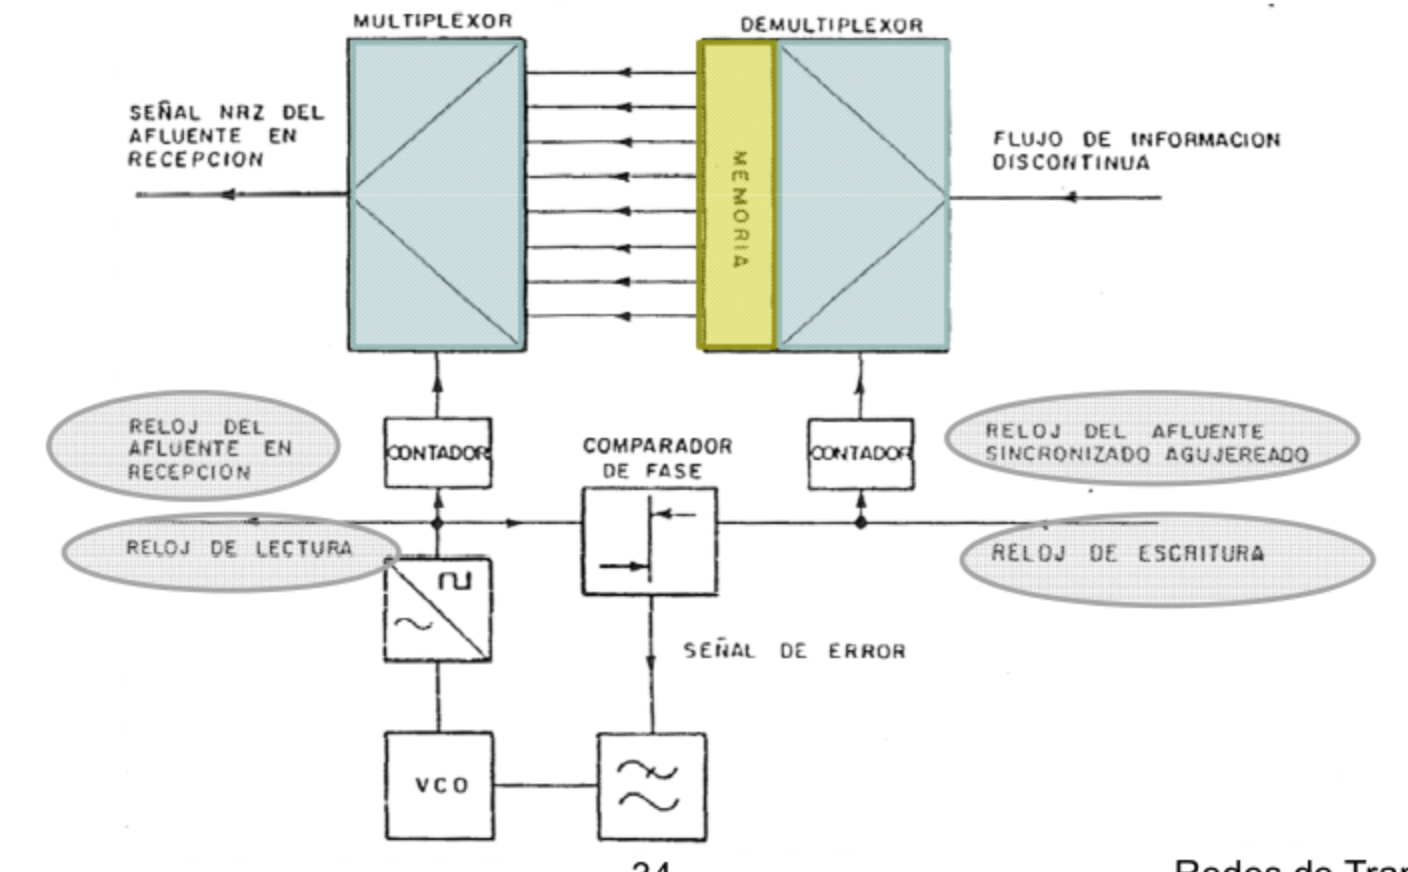
\includegraphics[width=0.35\textwidth]{Elastica2}
      \caption{Memorias Elásticas RX}
      \label{fig:Regiones de frecuencias}
  \end{figure}
\end{itemize}
  
 
\begin{figure}[!ht]
	\centering
     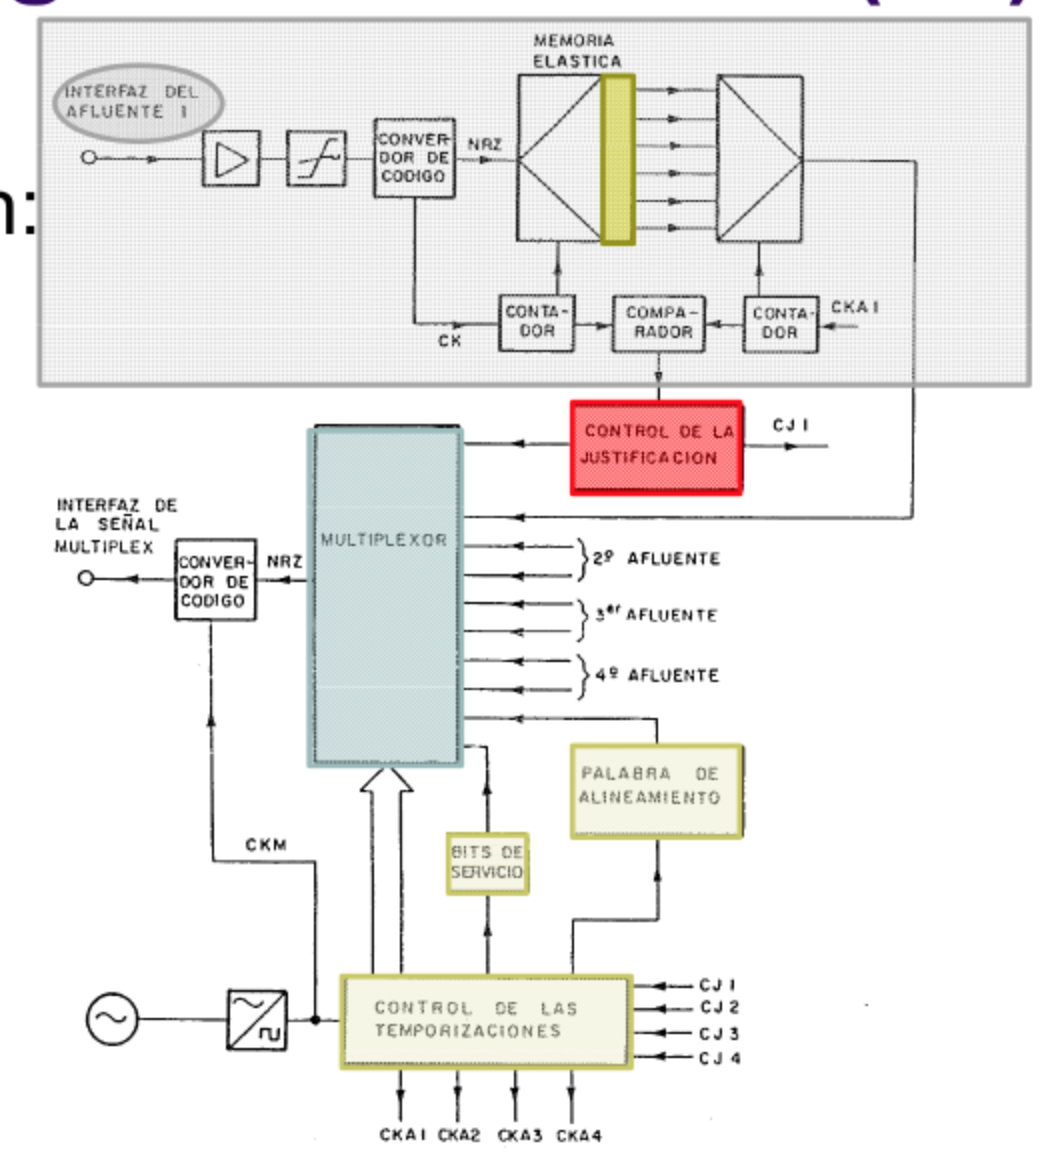
\includegraphics[width=0.35\textwidth]{muxtx}
      \caption{Esquema general del MUX TX}
      \label{fig:Regiones de frecuencias}
\end{figure}

\begin{figure}[!ht]
	\centering
     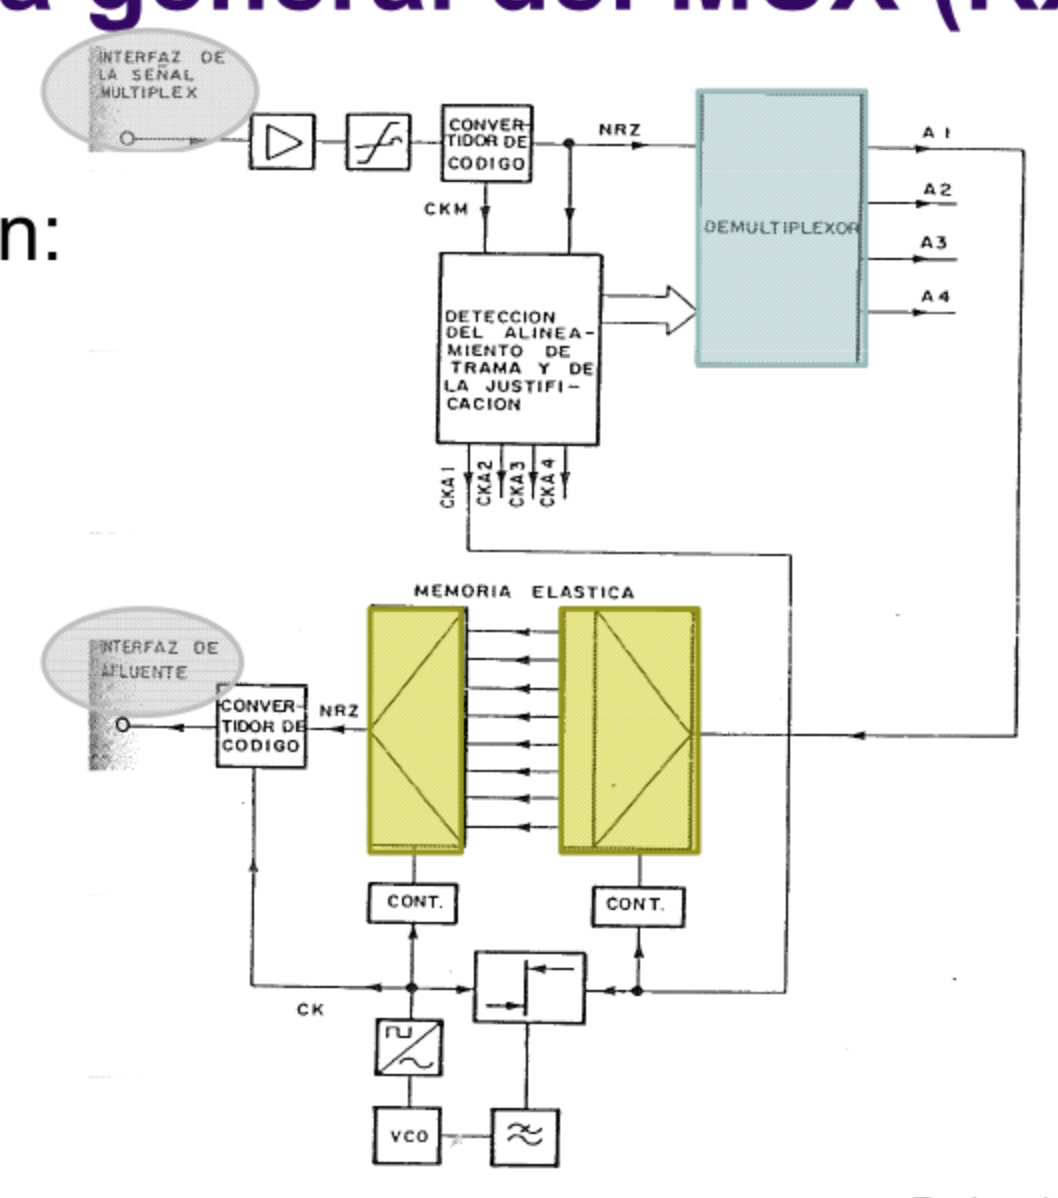
\includegraphics[width=0.35\textwidth]{muxrx}
      \caption{Esquema general del MUX RX}
      \label{fig:Regiones de frecuencias}
\end{figure}

\textbf{Velocidad de tributario}

\begin{figure}[!ht]
	\centering
     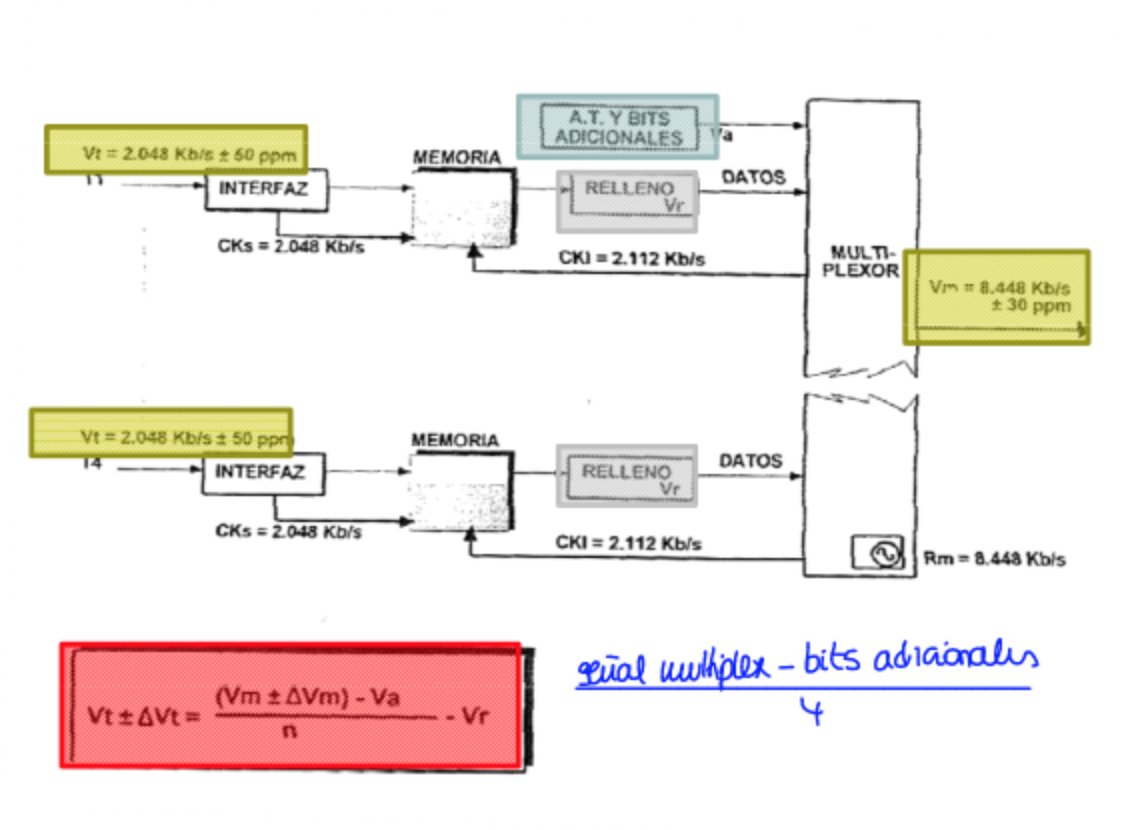
\includegraphics[width=0.5\textwidth]{tributario}
      \caption{Tributario}
      \label{fig:Regiones de frecuencias}
\end{figure}

\begin{itemize}
\item Velocidad de tributario: $V_{t}$
\item Justificación: $V_{r}$
\item Velocidad bits de alineamiento de trama y control de justificación: $V_{a}$
\item Plesiocronidad: $\Delta V_{m}$, $\Delta V_{t}$
\end{itemize}

\textbf{Multiplex Digital 2/8} es una estructura de trama de 8Mbits/seg (filas). En este caso hay 4 bits S que se pueden utilizar de relleno o justificación.

\begin{figure}[!ht]
	\centering
     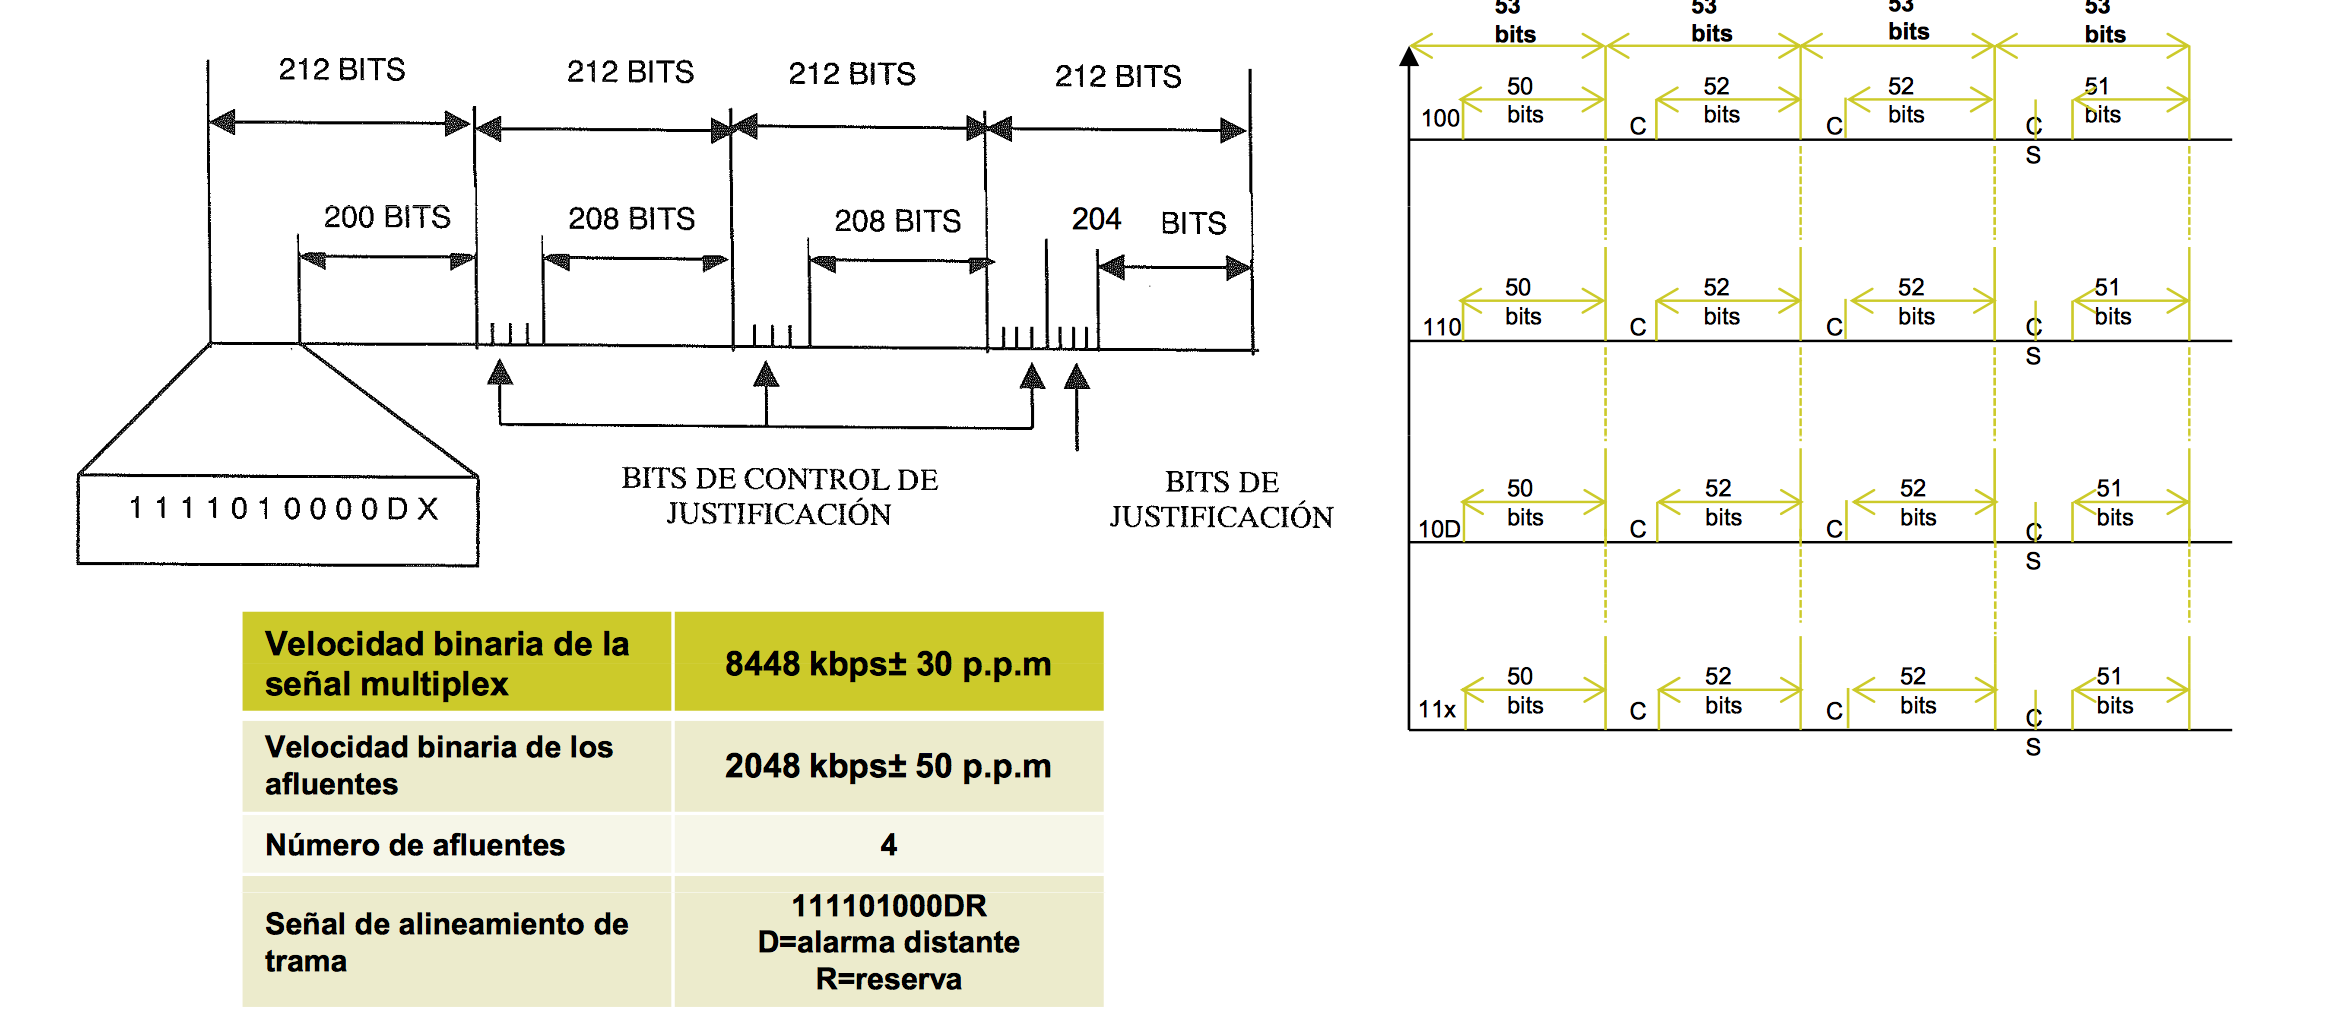
\includegraphics[width=0.5\textwidth]{mux28}
      \caption{Múltiplex Digital 2/8}
      \label{fig:Regiones de frecuencias}
\end{figure}

\begin{figure}[!ht]
	\centering
     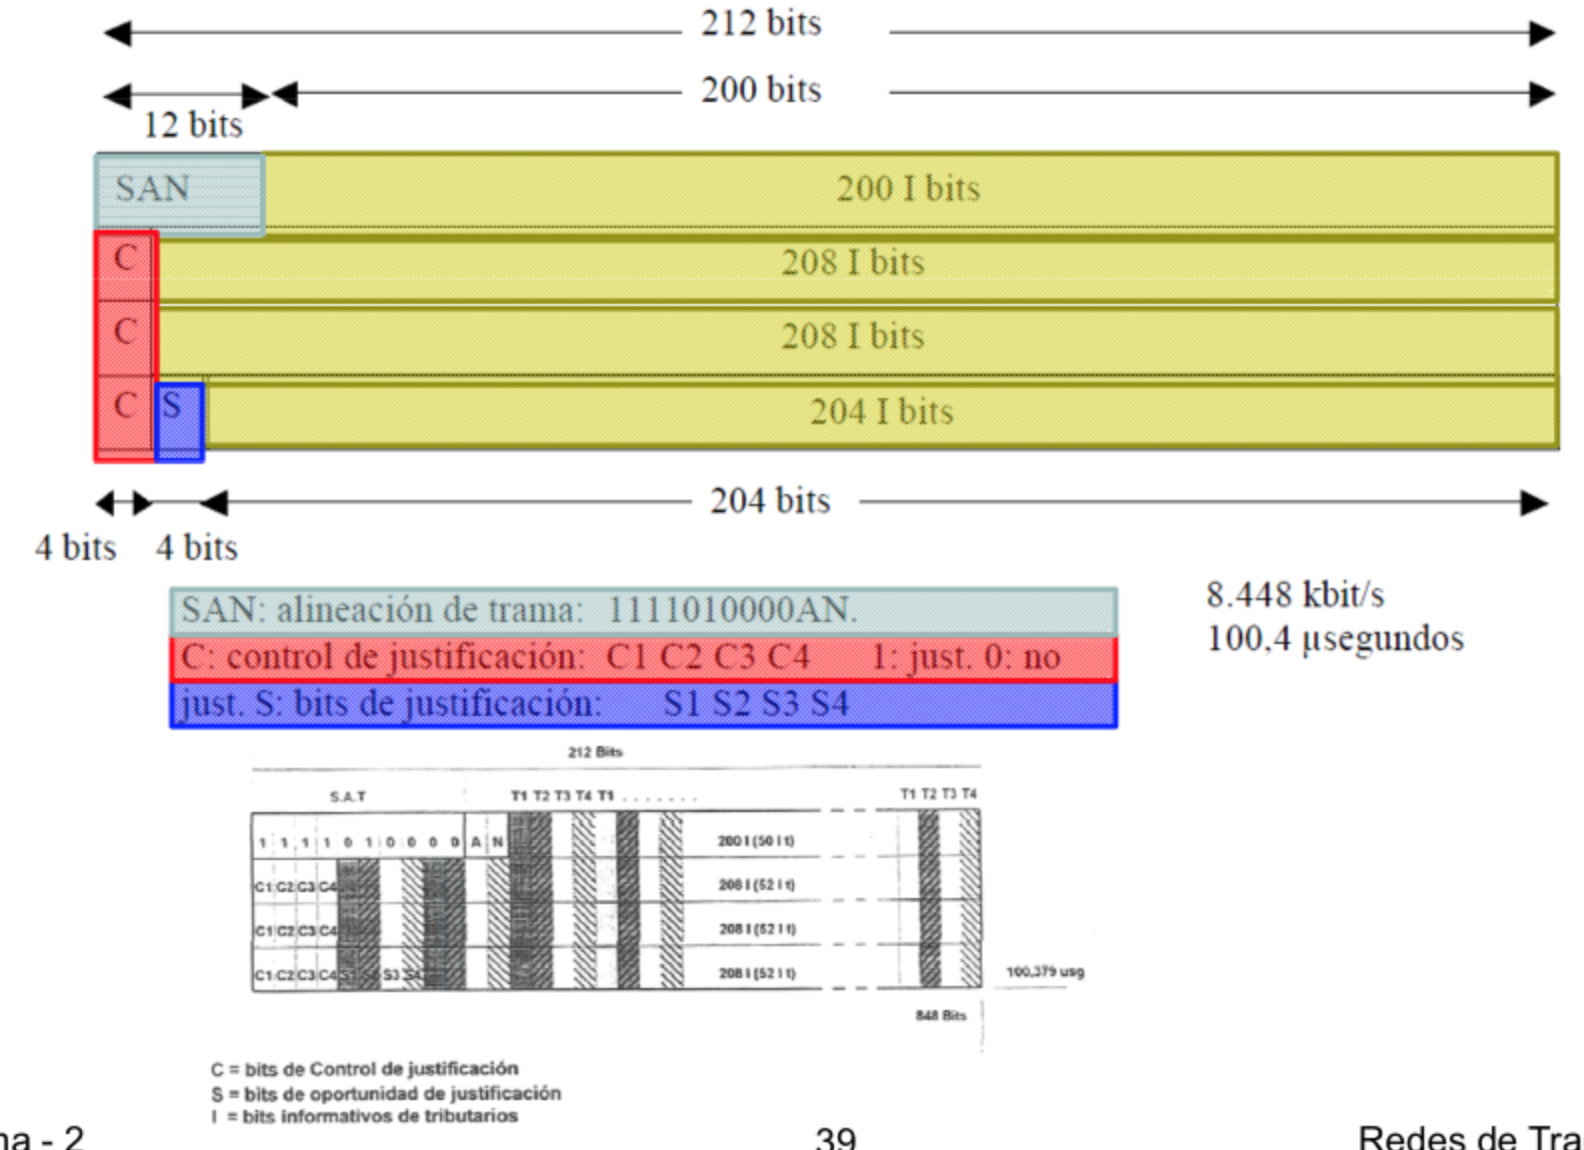
\includegraphics[width=0.5\textwidth]{otromux}
      \caption{Múltiplex Digital 2/8}
      \label{fig:Regiones de frecuencias}
\end{figure}

\textbf{Multiplex Digital 8/34}

\begin{figure}[!ht]
	\centering
     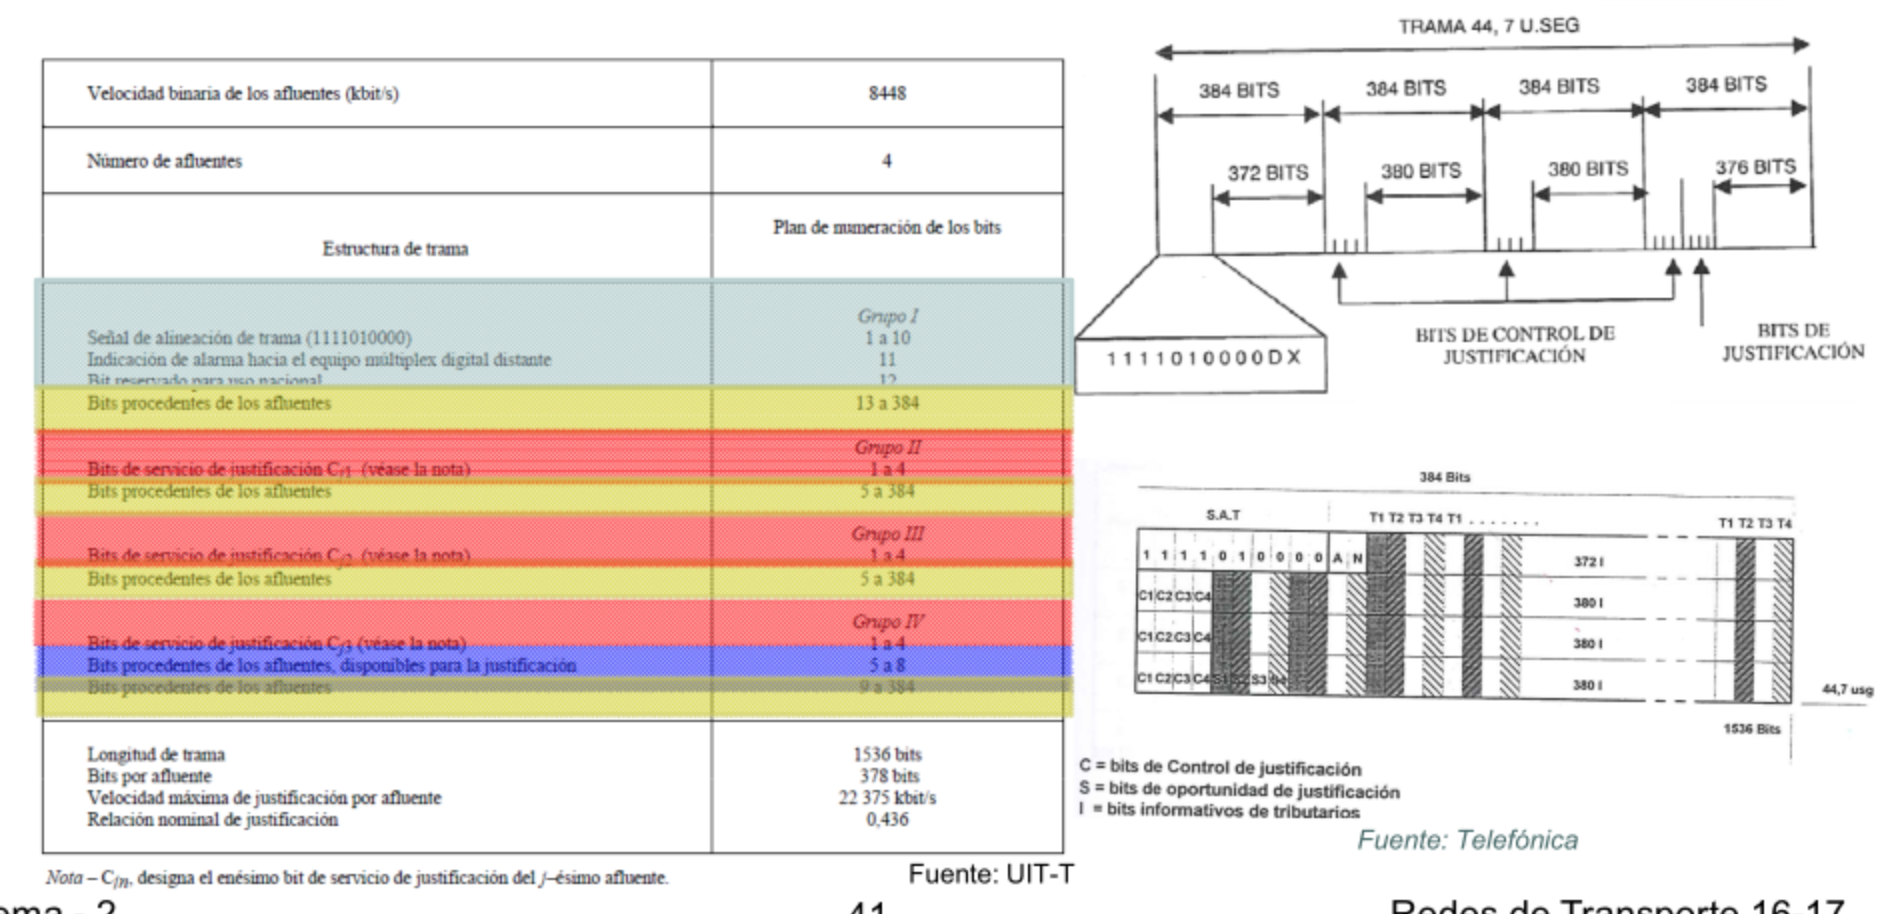
\includegraphics[width=0.5\textwidth]{mux834}
      \caption{Estructura de la trama de 34MBits/seg}
      \label{fig:Regiones de frecuencias}
\end{figure}


\begin{figure}[!ht]
	\centering
     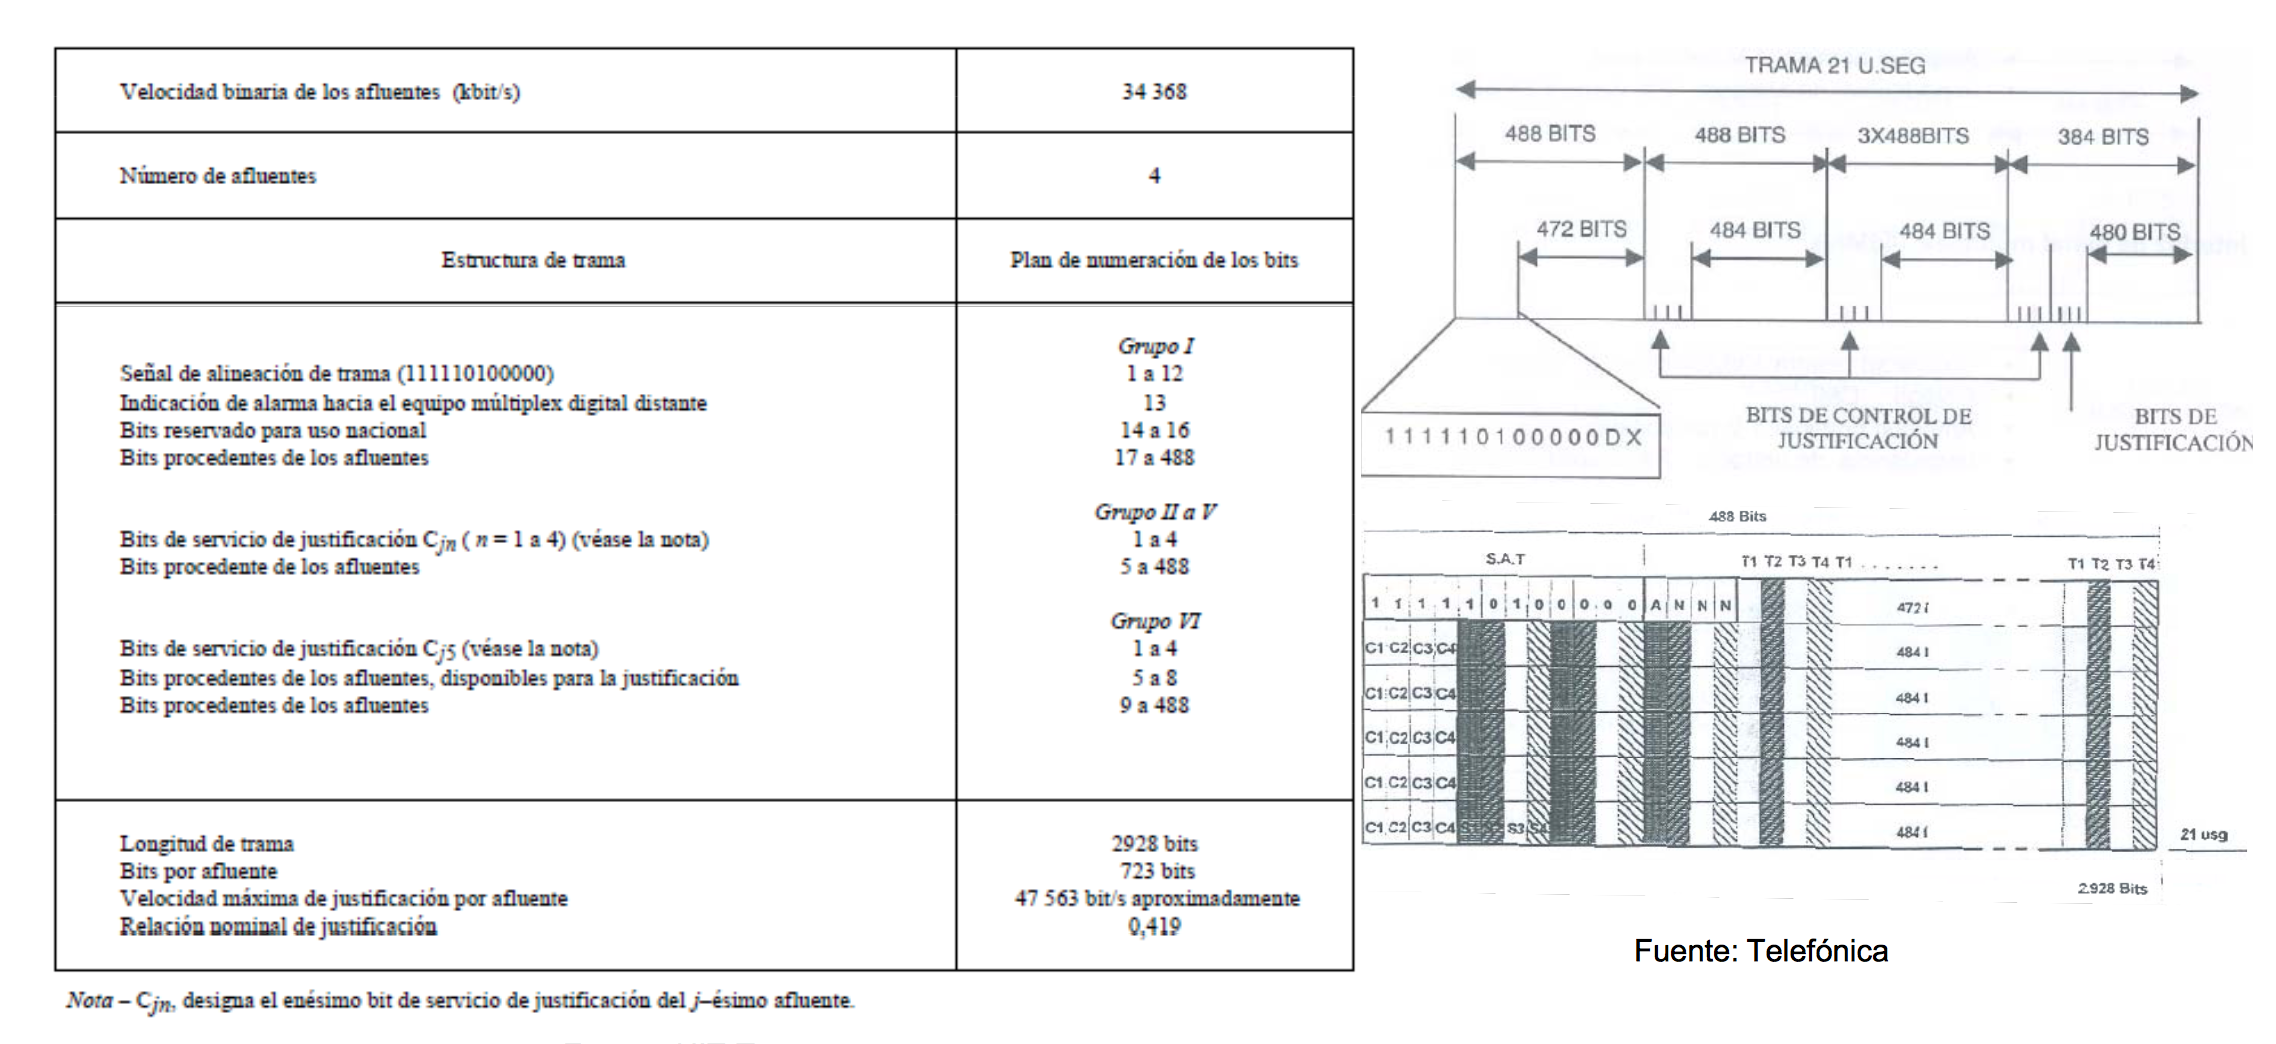
\includegraphics[width=0.5\textwidth]{trama140}
      \caption{Estructura de la trama de 140MBits/seg}
      \label{fig:Regiones de frecuencias}
\end{figure}

\textbf{Gestión de alarmas en PDH}:

	\begin{itemize}
		\item \textbf{LOS} (\textit{Loss Of Signal}): Pérdida de señal de entrada, se supera una tasa de error superior a $10^{-3}$.
		\item \textbf{LOF} (\textit{Loss of Frame}): Pérdida de alineamiento de trama, se detectan con error 4 palabras consecutivas y se produce la pérdida del alineamiento de trama LOF:
		\item \textbf{AIS} (\textit{Alarm Indication Signal}): Señal indicación de alarma, generada para reemplazar el tráfico normal cuando este contiene una condición defectuosa para poder prevenir fallos. Se utiliza para \textbf{detectar averías}. Si se detecta pérdida de señal de entrada en un afluente se manda señal SIA por los bits de la señal múltiplex correspondientes a ese afluente respetando la velocidad nominal de justificación de ese afluente. Si se detecta pérdida de señal de entrada en la señal múltiplex, o pérdi
		\item \textbf{RDI} (\textit{Remote Defect Indication}): Indicación de defecto remoto, se envía al equipo transmisor cuando se detectan alarmas como LOC, LOS o AIS.
		\item \textbf{HBER} (\textit{Hard BER}): Tasa de error grave, cuando se supera una tasa de error superior a $10^{-3}$.
	\end{itemize}

\begin{figure}[!ht]
	\centering
     \includegraphics[width=0.5\textwidth]{Errores}
      \caption{Gestión de Alarmas en PDH}
      \label{fig:Regiones de frecuencias}
\end{figure}

\textbf{PDH} tiene \textbf{limitaciones}:

	\begin{itemize}
	\item No permite extraer tributarios de baja capacidad de jerarquías superiores.
	
		\begin{center}
			\includegraphics[width = 0.25\textwidth]{images/Tributarios}
		\end{center}
	\item Complejidad de los nodos de conexión.
	\item Difícil operación, administración y mantenimiento.
	\item Jerarquías de alto nivel no estandarizadas.
	\item Difícil interconexión de redes de diferentes estándares.
	\item Baja capacidad.
	\end{itemize}
	
\subsection{SDH/SONET}

SDH soluciona el problema de la sincronización de PDH, el reloj maestro envía la señal a todos los nodos por la red.

\begin{tabular}{|r|l|l|}
\hline
                                   & \multicolumn{1}{c|}{\textbf{PDH}}              & \multicolumn{1}{c|}{\textbf{SDH}}                                            \\ \hline
\textbf{Velocidades}               & Distintas según zona geográfica.               & Universales.                                                                 \\ \hline
\textbf{Velocidad básica}          & 2 Mbps                                         & 155 Mbps                                                                     \\ \hline
\textbf{$V_{sig mux}$}             & $V_{sig mux} > 4 \cdot V_{sig afluentes}$      & $V_{sig mux} = n \cdot V_{STM-1}$                                            \\ \hline
\textbf{Multiplexación}            & Bit a bit                                      & Byte a Byte                                                                  \\ \hline
\textbf{Velocidades}               & Bajas                                          & Media                                                                        \\ \hline
\textbf{Medios de TX}              & Pares, coaxial y fibra                         & Fibra                                                                        \\ \hline
\textbf{Extracción de tributarios} & Mux/demux hasta el nivel requerido             & Facilidad para la extracción                                                 \\ \hline
\textbf{Topología}                 & Punto a punto                                  & Anillo                                                                       \\ \hline
\textbf{Compatibilidad}            & Incompatible entre fabricantes                 & Global                                                                       \\ \hline
\textbf{Sincronismo}               & Plesiócrona                                    & Síncrona                                                                     \\ \hline
\textbf{Bytes}                     & 2 de cada 32 bytes para gestión y señalización & Prima la compatibilidad por encima de la eficiencia. Muchos bytes de gestión \\ \hline
\textbf{Alarmas}                   & Limitada                                       & Potente                                                                      \\ \hline
\end{tabular}

\textbf{Características} de \textbf{SDH}:

\begin{itemize}
\item La trama SDH es el \textbf{módulo de transporte síncrono} STM. 
\item La \textbf{duración de la trama es uniforme} ($125 \mu s$) y es independiente de la velocidad. 
\item Hay carga útil en el \textbf{contenedor}. 
\item Multiplexación sencilla, byte a byte. 
\item \textbf{Acceso a tributarios} sin demultiplexación. 
\item \textbf{Reloj de referencia} para toda la red. 
\item Alto grado de estandarización.
\item  Velocidades \textbf{desde 155Mbps hasta 40Gbps}.
\item  Tratamiento a nivel de byte. 
\item Utilización de \textbf{punteros}. 
\item Canales de servicio y supervisión de gran capacidad. 
\item Fácil adaptción a servicios de banda ancha y a DWDM. 
\item Hay tres redes: Transmisión, sincronización y gestión.
\end{itemize}

\textbf{SONET/SDH} fueron diseñadas en principio para transportar señales PDH. Ahora está adaptada a señales de banda ancha.\\

La red SDH se divide en \textbf{capas}:

	\begin{itemize}
	\item \textbf{Capa física}: Medio de transmisión
	\item \textbf{Sección de regeneración}: Tramo entre regeneradores, RSOH. Es el tramo de la red de transmisión comprendido entre dos equipos de transmisión que regeneran la señal (todo). Insertan y extraen RSOH (\textit{Regeneration Section OverHead}).
	\item \textbf{Sección de multiplexación}: Tramo entre multiplexores, MSOH. Es el tramo de la red de transmisión comprendido entre los puntos de multiplexado/demultiplexado del STM-N. Insertan/extraen MSOH (\textit{Multiplex Section Overhead}).
	\item \textbf{Trayecto}: Tramo de la red comprendiendo entre los puntos de ensamblado y desensamblado de los CVs. Es el tramo de la red de transmisión comprendido entre los puntos de ensamblado y desensamblado de los contenedores virtuales. Insertan y extraen POH (\textit{Path OverHead}).
	\end{itemize}


\textbf{Módulo de Transporte Síncrono STM-1} (\textit{Synchronous Transport Module}:

	\begin{itemize}
	\item Primer nivel jerárquico básico
	\item Compuesto de campos de información y campos de gestión
	\item Duración de la trama $125 \mu s$
	\item Longitud de 2430 octetos
	\item Velocidad binaria 155.520 (2.430 * 8)/125 * 10-6=155.520 Kb/s).
	\item Interfaz eléctrico u óptico.
	\item Velocidades superiores interfaz siempre óptico.
	\end{itemize}
	
\textcolor{red}{STM-X}

Un \textbf{contenedor} es una unidad definida de capacidad útil, dimensionada para poder transportar señales PDH y otras señales de banda ancha. Un contenedor está compuesto por relleno y carga útil.\\

Un \textbf{contenedor virtual} es el nombre con el que se designa a un tributario SDH transportado en una señal STM-1 (C + POH).\\

Una \textbf{unidad tributaria (TU)} es una subdivisión del espacio de carga de un contenedor virtual de orden superior (VC + Puntero).\\

Un \textbf{grupo de unidades tributarias (TUG)} son una o más TU que ocupen posiciones fijas y definidas en un contenido útil de orden superior.\\

Una \textbf{unidad administrativa (AU)} es una subdivisión del espacio de carga de la trama de línea (VC + Puntero de AU).\\

Un \textbf{grupo de UAs} son una o más AUs que ocupan posiciones fijas.

\begin{figure}[h]
	\centering
     \includegraphics[width=0.15\textwidth]{STM1}
      \caption{Flujograma STM-1 (sin UT)}
      \label{fig:STM1}
\end{figure}

Las \textbf{taras o encabezados} son octetos reservados para la información del propio sistema.

	\begin{itemize}
	\item \textbf{Tara de Trayecto (POH)}: Se asigna al contenido útil al multiplexarse y permanece con ese contenedor hasta que se demultiplexa.
	\item \textbf{Tara de sección (SOH)}: Forma parte de la trama STM y está dividida en dos partes:
		\begin{itemize}
		\item Tara de sección de multiplexación (MSOH)
		\item Tara de sección de regeneración (RSOH)
		\end{itemize}
	\end{itemize}
	
Hay una \textbf{necesidad de punteros}, aunque es síncrono idealmente no lo es. Un \textbf{puntero} es un número binario situado en posiciones fijas, que va a indicar a qué distancia del inicio del área de carga se encuentra el primer octeto del VC. Desempeñan dos funciones:

	\begin{itemize}
		\item Identifican la posición de los VC en la trama
		\item Adaptan la velocidad binaria de los VCs a la velocidad binaria del canal de transmisión (AU o TU), utilizando mecanismos de justificación.
		\item Permiten asignar de forma flexible y dinámica los distintos VCs dentro del área de carga de unidades. 
		\item Permiten absorber mediante un mecanismo de justificación positiva/negativa, las diferencias de frecuencia.
	\end{itemize}
	
\textbf{Procesos para el transporte síncrono en SDH}:

	\begin{itemize}
	\item \textbf{Entramado/Mapeado}: Proceso mediante el cual se adaptan, dentro de los contenedores virtuales, las señales JDL, las células ATM u otras señales. Consiste en acomodar la sseñales de acceso correspondientes en los contenedores apropiados.
	\item \textbf{Alineamiento}: Procedimiento basado en la técnica de punteros, mediante el cual se permite identificar las posiciones de los VC en la trama que los contiene. Consiste básicamente en asociado a un contenedor virtual un puntero para obtener una unidad administrativa o una unidad tributaria.
	\item \textbf{Multiplexación}: Consiste en combinar, por medio del entrelazado simple de octeto, varias TU, para obtener un TUG (o varios) para formar otro TUG o un VC de orden superior.
	\end{itemize}


La \textbf{estructura de multiplexación} se basa en el procedimiento de entrelazado de octetos de los diferentes elementos a multiplexar.

\textcolor{red}{TERMINAR}

\textbf{Equipos en SDH}:

	\begin{itemize}
	\item \textbf{Regeneradores}: Regeneran el reloj y la amplitud de las señales de datos. Recupera la señal digital y vuelve a codificarla con el código de línea. Procesa la RSOH.
	\item \textbf{ADM}: Insertan y extraen señales de menor velocidad a partir del flujo SDH de alta velocidad. Habilitan las estructuras en anillo que permiten la conmutación automática. Multiplexa plesiócrona en una señal STM-N. Procesa toda la estructura SDH. Algunos fabricantes no tienen regeneradores ni TS específicos, se usan ADMs. Realiza las mismas funciones que un TS. Conecta VCs entre los distintos interfaces (agregado - agregado, tributario - agregado, tributario - tributario).
	\item \textbf{TS (Terminal Síncrono)}: Combinan las señales de entrada PDH y SDH en señales STM-N de mayor velocidad.
	\item \textbf{DXC/DCS (Digital Crossconnect System)}: Interconectan cualquier canal de un puerto determinado con cualquier otro canal de puertos diferentes. Realiza las mismas funciones que un ADM pero con N agregados. 
	\end{itemize}
	
Las \textbf{ventajas} de \textbf{SDH}:
	
		\begin{itemize}
		\item Mucha información para el control, gestión y operación. Gestión de alarmas.
		\item Seguridad: Facilidades de protección y restauración automática (anillos ópticos). 
			\begin{itemize}
			\item La diversificación consiste en dividir el número de circuitos habilitando dos rutas con capacidad de tráfico de algo más de 50\%.
			\item Protección. Recuperación automática ante fallos. La solución está prevista. Se realiza mediante mensajes del protocolo APS (Automatic Protection Switching) mediante los bytes \texttt{K} de las cabeceras. Tipos: Protección de sección de multiplexación, protección de trayecto y protección de subred.
			\end{itemize}
		\item Adaptación a nuevos servicios de banda ancha (NG-SDH).
		\end{itemize}

\section{Transmisión en Redes de Datos}

\subsubsection{Jerarquías de Multiplexación Ópticas}

\textbf{WDM} (\textit{Wavelength Division Multiplexing}) multiplexa varias señales sobre una sola fibra óptica mediante portadoras ópticas de diferente longitud de onda, empleando luz procedente de un láser o un LED.

	\begin{itemize}
		\item CWDM (Coarse WDM)
		\item DWDM (Dense WDM)
	\end{itemize}
	
\textbf{Elementos} de un sistema:
	
	\begin{itemize}
	\item \textbf{Transpondedor}: Convierte la señales eléctricas de los sistemas clientes en señales ópticas sobre longitudes de onda disponibles en sistemas WDM. Si la señal de entrada ya pertenece al dominio óptico de banda ancha, el transpondedor se encarga de adaptar las longitudes de onda recibidas a una longitud de onda estandarizada, estabilizada y susceptible de ser multiplexada y demultiplexada. Conecta/adapta un sistema cliente de la red óptica, realiza la conversión Óptica-Eléctrica-Óptica. Cada transpondedor dentro de un sistema WDM, convierte la señal ``cliente'' en una longitud de onda levemente diferente. Las longitudes de onda provenientes desde todos los transpondedores de un sistema son entonces multiplexadas óptica. Hay tres generaciones: 1R, 2R y 3R\footnote{Reamplificación, retemporización y regeneración}. El \textbf{muxponder} es un transponder pero con el agregado de un multiplexor que multiplexa las señales clientes de menor jerarquía de una mayor jerarquía.
	\item \textbf{Multiplexor}: Multiplexa las longitudes de ondas que provienen del transpondedor/entrada en una sola señal óptica. Equipos multiplexores:
		\begin{itemize}
		\item Multiplexor WDM
		\item OADM (Multiplexor óptico de Inserción/Extracción)
		\item OXC (Optical Cross-Conect)
		\end{itemize}
	\item \textbf{Amplificador}: Amplifica un conjunto de longitudes de onda. Amplifica la señal óptica multiplexada, antes de su transmisión por la fibra óptica.
		\begin{itemize}
		\item \textbf{SOA} (\textit{Semiconductor Optical Amplifier}) Amplificador de banda ancha para amplicaciones en segunda vendana o CWDM. Son de baja potencia de salida y bastante ruidosos y no lineales. De uso restringido.
		\item \textbf{EDFA} (\textit{Erbium Dopped Fiber Amplifier}): Amplificador óptico para aplicaciones monocanal o multicanal DWDM. De uso más común.
		\item \textbf{RAMAN}: Amplificadores ópticos de ultrabajo ruido. Se utilizan en combinación con EDFAs en aplicaciones monocanal o DWDM para enlaces de ultra larga distancia sin posibilidad de regeneración o amplificación intermedias.
		\end{itemize}
	\end{itemize}
	
WDM tiene un \textbf{problema} y es que no proporciona mecanismos de gestión y protección. La \textbf{solución} es \textbf{OTN} (\textit{Optical Transport Network}). Al igual que SDH, proporciona tara para el control de las conexiones en ambos extremos y por varios segmentos del enlace. Dicha tara incluye la identificación de la señal, la medición de errores y la información de alarma.

\quad Pueden envolver (\textit{digital wrapper}) cualquier servicio en un contenedor digital óptico y permitir así la transparencia de servicio que ofrece la flexibilidad para dar soporte a todo tipo de tráfico.

\quad Combina la multiplexación óptica y eléctrica en una infraestructura común y preparada para el futuro con funcionalidades de gestión como las jerarquías digitales.

\quad Permite un funcionamiento, una administración y una gestión que son transparentes para sus clientes. Pueden transportar cualquier tipo de tráfico de paquetes de datos. Las tramas OTN pueden transportar tramas SDH completas, incluida la tar de señal del cliente sin modificación. \\

\textbf{Sección de red:}

	\begin{itemize}
	\item Sección de transporte óptico (OTS)
	\item Sección de multiplexación óptica (OMS)
	\item Canal Óptico (Och)
	\end{itemize}
	
\textbf{Unidades de datos} de OTN:

	\begin{itemize}
	\item OPU: Optical Channel Payload Unit
	\item OTU: Optical Channel Transport Unit
	\item ODU: Optical Channel Data Unit
		\begin{itemize}
		\item Cabecera
			\begin{itemize}
			\item PM (\textit{Path Monitoring}): La cabecera de supervisión de trayecto de ODU permite la monitorización de secciones determinadas dentro de la red así como la localización del fallo en la red vía los octetos descritos en la cabecera supervisión de trayecto PM.
			\item TCM (\textit{Tandem Connection Monitoring}): La supervisión de conexión en cascada, es una función que hace posible la gestión de la señal a través de múltiples redes. También usa los bytes de paridad para comprobar errores.
			\end{itemize}
		\end{itemize}
	\end{itemize}

Cabecera de ODU (PM y TCM):

	\begin{itemize}
	\item Identificador de traza de camino (TTI-Trail Identifier). Usado para reconocer la señal de origen al destino en de la red: Identificador de Punto de Acceso de Origen (SAPI - Source Address Point Identifier) y el indicador del punto de acceso de destino (DAPI - Destination Access Point Identifier).
	\item Paridad de entrelazado de bits-nivel 8 BIP-8 (Bit Interleaved Parity. Este es un byte que se usa para la detección de error.
	\item Indicador de defecto hacia atrás (BDI - Backward Defect Indicacion). Es un solo bit que brinda información del fallo de la señal en dirección hacia atrás.
	\item Indicador de error hacia atrás (BEI - Backward Error Indication) y error de alineación entrante hacia atrás (BIAE - Backward Incoming Alignment Error). Este indicador trae consigo información acerca de los bloques de entrelazado de bit detectados con error en la dirección hacia atrás.
	\end{itemize}

Cabecera de ODU (FTFL):

	\begin{itemize}
	\item Canal de comunicación de informe de localización de fallo y tipo de fallo (fTFL - Fault Type y Fault Location Channel). Permite transmitir un mensaje de 256 bytes del estado de la falla tanto información en cuanto al tipo y ubicación de ésta.
	\end{itemize} 
	
Cabecera OTU (OTU-OH):

	\begin{itemize}
	\item Compuesta por la sección de monitoreo (SM), canal de comunicaciones 0 (GCC0), y se reservan 2 bytes.
	\end{itemize}

La \textbf{trama OTH} está constituida por tres partes diferenciadas:
	\begin{itemize}
	\item Cabeceras de gestión:
		\begin{itemize}
		\item OPU OH
			\begin{itemize}
			\item PSI (\textit{Payload Structure Identifier}): Transporta un mensaje de 256 bytes alineados con la multitrama ODU
			\item PT: Tipo de señal de cliente
			\end{itemize}
		\item OTU OH
		\item ODU OH
		\end{itemize}
	\item Carga útil
	\item Datos FEC (\textit{Forward Error Correcting})
	\end{itemize}

\textbf{Velocidades binarias OTH}:
	\begin{itemize}
	\item No hay señales ópticas (OCh/OTUk) asociadas con ODU0, ODU2e y ODUflex. Esta señales ODU se transportan en uno o más intervalos subordinados de una señal ODUk de velocidad superior que tiene una OTUk correspondiente.
		\begin{itemize}
		\item La velocidad ODU0 ha sido optimizada para transportar una señal de cliente Ethernet a 1 Gbit/s y dos señales ODU0 en una ODU1.
		\item La velocidad ODU2e ha sido optimizada para transportar una señal de cliente Ethernet a 10Gbit/s.
		\item La velocidad ODUflex peude ser cualquier valor en un rango hasta la velocidad binaria de la mayor zona de cabida útil OPUl. La ODUflex ha sido introducida para transportar cualquier futura señal CBR o de cliente en paquetes de la manera más óptica posible.
		\end{itemize}
	\end{itemize}
	
\textbf{Plano de control OTN} (GMPLS) se posibilita calcular automáticamente el camino óptico para la señal cliente.\\

\textbf{MPLS-TP} (\textit{MultiProtocol Label Switching - Transport Profile}. Razones para la transmisión de TDM a IP/Ethernet:

	\begin{itemize}
	\item La mayor parte de tráfico en redes actuales es tráfico de datos en ráfagas.
	\item Limitación de capacidad de SDH.
	\item Coexistencia de redes tradicionales TDM y nuevas redes puede resultar muy cara y compleja de operar.
	\end{itemize}

\textbf{?`Por qué MPLS-TP en vez de Ethernet?} 
	\begin{itemize}
	\item Sobre el entramado GFP es más eficiente a nivel de transporte que el entramado de Ethernet.
	\item Utiliza una pila jerarquizada para el etiquetado que permite una clara separación entre niveles facilitando, por otro lado, la interoperabilidad entre los niveles.
	\item Permite configuraciones tanto estáticas como dinámicas gracias al plano de control GMPLS.
	\item Permite la gestión de la reserva del ancho de banda, la gestión de múltiples parámetros de QoS e incluye mecanismos de restauración en tiempos similares a SDH.
	\item Facilita la migración de las redes actuales (IP/MPLS) sobre SDH que utilizan MPLS-TE (\textit{MPLS - Traffic Engineering}).
	\end{itemize}
	
MPLS-TP:
	\begin{itemize}
	\item Utiliza sólo un subconjunto (``profile'') de las funcionalidades MPLS.
	\item Posibilita la implantación de MPLS en las redes de transporte con un grado de gestión, fiabilidad y O+m similar al que podemos encontrar en las redes de transporte basadas en TDM de hoy día (SONET/SDH).
	\item Asegura compatibilidad con IP/MPLS.
	\end{itemize}
	
\textbf{Introducción a MPLS}:
	\begin{itemize}
	\item Basado en el etiquetado de los paquetes en base a criterios de prioridad y/o calidad.
	\item Su idea es realizar la conmutación de los paquetes o datagramas en función de las etiquetas añadidas en la capa 2 y etiquetar dichos paquetes según la clasificación establecida por la QoS.
	\item Trata de proporcionar algunas de las características de las redes orientadas a conexión a las redes no orientadas a conexión.
	\item En el encaminamiento IP tradicional (sin conexión), la dirección de destino junto a otros parámetros de la cabecera, es examinada cada vez que el paquete atraviesa un router. La ruta del paquete se adapta en función del estado de las tablas de encaminamiento de cada nodo, pero, como la ruta no puede predecirse, es difícil reservar recursos que garanticen la QoS.
	\item Las búsquedas en tablas de encaminamiento hacen que cada nodo pierda cierto tiempo, se incrementa en función del tamaño de la tabla.
	\item Permite a cada nodo, ya sea un switch o un router, asignar una etiqueta a cada uno de los elementos de la tabla y comunicarla a sus nodos vecinos. 
	\item Esta etiqueta es un valor corto y de tamaño fijo transportado en la cabecera del paquete para identificar un FEC, que es un conjutno de paquetes que son reenviados sobre el mismo camino a través de la red, incluso si sus destinos finales son diferentes.
	\item La etiqueta es un identificador de conexión que sólo tiene significado local y que establece una correspondencia entre el tráfico y un FEC específico. Dicha etiqueta se asigna al paquete basándose en su dirección de destino, los paráetros de tipo de servicio, pertenencia a VPN o cualquier otro criterio.
	\item Cuando MPLS está implementado como una solución IP pura o de nivel 3, la etiqueta es un segmento de información añadido al comienzo del paquete.
	\end{itemize}
	
\textbf{Campos de cabecera MPLS}:
	\begin{itemize}
	\item Label (20 bits): Identificación de la etiqueta
	\item Exp (3 bits): Llamado también bits experimentales, también aparece como QoS, afecta al encolado y descarte de paquetes.
	\item S (1 bits): Stack, sirve para el apilado jerárquico de etiquetas. Cuando S = 0 indica que hay más etiquetas añadidas al paquete. Cuando S=1 se ha llegado al fondo de la jerarquía.
	\item TTL (8 bits): Time-to-Live).
	\end{itemize}
	
\textbf{Terminología} MPLS:

	\begin{itemize}
	\item LER: Label Edge Router
	\item LSR: Label Switch Router
	\item LSP: Label Switched Part
	\end{itemize}
	
MPLS-TP funcionalidades:

	\begin{itemize}
	\item \textbf{Plano de datos} basado en MPLS ``\textit{label forwarding}'':
		\begin{itemize}
		\item Push: Se añade una etiqueta saliente
		\item Pop: Se quita la etiqueta entrante
		\item Swap: Se reemplaza la etiquete entrante por la etiqueta saliente.
		\end{itemize}
	\item \textbf{Plano de control} basado en GMPLS (Global MPLS)
	\end{itemize}
	
\subsection{Transmisión en Redes de Datos}

\subsubsection{Introducción}

\subsubsection{Ethernet sobre la capa de transporte (EoT)}

Ethernet fue una de las primeras tecnologías de red de zona local (LAN) y ha prosperado hasta convertirse en la tecnología LAN predominante. La omnipresencia de Ethernet en empresas hace que proveedores de servicio ofrezcan la conectividad Ethernet en múltiples sitios. Como consecuencia, Ethernet se está transformando en el mecanismo de transporte del operador dentro de las propias redes de los proveedores de servicios de datos, dado que el mayor crecimiento en estas redes se está viendo impulsado por aplicaciones tales como el vídeo digital y otros muchos servicios de datos. En estos casos, los clientes exigen servicios de calidad de servicio (QoS) y una elevada disponibilidad.  Nuevas normas, como PBB-TE (\textit{Provider Backbone Bridge - Traffic Engineering}) permiten utilizar Ethernet como mecanismo de transporte (\textit{Carrier Ethernet}).\\

\textbf{PBB-TE} proponeextensiones de Ethernet que permitan resolver los problemas inherentes a Ethernet respecto a escalabilidad, QoS y disponibilidad. 

	\quad En el estándar 802.1 ah se incluye:
	
		\begin{itemize}
		\item Nueva MAC de transporte (Mac-in-Mac)
		\item Túneles con camino explícito, QoS y recuperación en 50ms.
		\item Se desactivan ciertas funciones, como broadcasting, aprendizaje de MACs y funcionalidad del Spanning Tree.
		\end{itemize}

Finalmente, convertir Ethernet en orientada a conexión y con encaminamiento explícito y restauración impone nuevos requisitos:

	\begin{itemize}
	\item Necesario sustituir el Spanning Tree por un plano de control, con encaminamiento y señalización.
	\item En progreso de estandarización de un plano de control para redes Ethernet.
	\end{itemize}
	
No ha tenido mucha aceptación por la industria y parece que MPLS-TP es la apuesta.\\

Hay \textbf{alternativas} al \textbf{transporte de Ethernet} como SDH u OTN utilizando el procedimiento de entramado genérico (GFP - \textit{Generic Framing Procedure}).\\

\textbf{GFP} (\textit{General Framing Procedure}) proporciona un mecanismo genérico para adaptar tráfico de señales de cliente de alto nivel en una red de transporte. Es adecuado para el transporte de señales cliente Ethernet.

\subsection{Convergencia de Redes y Servicios: NGN}





\newpage

%%%%%%%%%%%%%%%%%%%%%%%%

\begin{framed}
	\begin{center}
    	\Large{\underline{Redes de Transporte}} \\
    	\scriptsize{3º Ingeniería de Telecomunicaciones | UPV/EHU}\\
     	%Actualizado por última vez el \today \\
     	"\textsl{Under-promise and over-deliver}." \\
     	%\hspace{5 pt} \\
     	\small{\textbf{Javier de Martín -- 2016}}
	\end{center}
\end{framed}

\section{Conmutacion}

\subsection{Conmutacion}

\subsubsection{Introducción}

Originalmente, la red telefónica se desarrolló para proporcionar la transmisión bidireccional de voz, para ello había líneas dedicadas entre cada pareja de usuarios siendo esto muy costoso y poco escalable. La solución a esto son los \textbf{conmutadores} que establecen circuitos temporales entre pares de usuarios.

\quad Hay una \textbf{estructura jerárquica de conmutadores} en la que mediante una red de tránsito se interconectan conmutadores.\\

El \textbf{objetivo} de la conmutación en las redes es interconectar a todos los usuarios de una red de telecomunicaciones a un coste razonable sin la necesidad de conectar directamente dos a dos.

\quad Esto se consigue mediante equipos (conmutadores) que van conmutando la información, tramo a tramo, desde cualquier origen hasta cualquier destino. Los conmutadores sirven para proporcionar caminos temporales para enviar información entre cualquier par de terminales conectados a la red. Para hacer esto hay que hacer uso de enlaces multiplexados entre los conmutadores.

\subsubsection{Tipos de Conmutación: Circuitos/Paquetes}

Según los \textbf{procedimientos que se usan} para conmutar la información de un enlace a otro:

\begin{itemize}
	\item \textbf{Conmutación de circuitos}: Se establece una conexión física entre el origen y el destino, al a que se le asignan recursos durante todo el tiempo que dura la comunicación. Cada conmutador mantiene establecida una conexión entre un canal de entrada y un canal de salida todo el tiempo que dura la comunicación. Es equivalente a tener un enlace punto a punto entre origen y destino.
	\item \textbf{Conmutación de paquetes}: Los datos a transmitir se estructuran en paquetes que además de los datos llevan información de control. Cada vez que un conmutador recibe un paquete por el enlace, en función de la información de control decide por qué enlace tiene que enviarlo, y lo pone en la cola de salida para ese enlace (a la espera de que le llegue el turno para ser enviado por el enlace).
	
	\begin{itemize}
		\item \textbf{Orientada a Conexión (Modo CV)}: Antes de enviar paquetes entre origen y destino, se fija el camino que van a seguir dichos paquetes (el camino es el CV) $\rightarrow$ ese camino queda escrito en las tablas de conexiones de los conmutadores. Fase previa de establecimiento del circuito virtual. Una vez establecido el circuito virtual, el resto de paquetes de la conexión son conmutados siguiendo las indicaciones de las tablas de conxiones.
		\item \textbf{No Orientada a la Conexión. Modo Datagrama}: Cada vez que llega un paquete a un conmutador, se decide por qué enlace de salida hay que enviarlo (los conmutadores de la red no consideran los diferentes paquetes como parte de una misma conmutación).
	\end{itemize}
\end{itemize}

\subsection{Conmutadores de Circuitos}

\begin{figure}[h]
	\centering
     \includegraphics[width=0.15\textwidth]{Bloque}
      \caption{Estructura a grandes bloques de un conmutador de circuitos}
      \label{fig:Regiones de frecuencias}
\end{figure}

La \textbf{red de conexiones (o matriz de conexiones)} proporciona, entra cualquier pareja de canales de E/S, un camino transparente para la señal. También proporciona un soporte físico de la comunicación.

%\begin{figure}[h]
%	\centering
%     \includegraphics[width=0.2\textwidth]{Matriz}
%      \caption{Matriz de conexiones}
%      \label{fig:Matriz}
%\end{figure}

\subsubsection{Conmutación espacial/temporal/bidimensional}

La \textbf{conmutación espacial} permite establecer una conexión entre un canal de entrada y un canal de salida a través de un camino físicamente separado y dedicado. La matriz de conexiones tiene $N^{2}$ puntos de cruce que pueden estar activos o inactivos. Si las entradas/salidas son multiplexadas en el tiempo \footnote{Por ejemplo MIC}, las conexiones no se mantienen durante todo el tiempo que dura la llamada sino que se van alternando cada intervalo de la trama. En cada uno de los diferentes intervalos hay diferentes puntos de cruce activos.

\quad La \textbf{Memoria de Control} indica al conmutador cuáles son los puntos de cruce que deben de estar activos en cada intervalo de tiempo de la trama $\rightarrow$ qué enlace de entrada  conmutar a qué enlace de salida.

	\begin{itemize}
		\item \textbf{CAE}:
		\item \textbf{CAS}:
	\end{itemize}

\begin{figure}[h]
	\centering
     \includegraphics[width=0.4\textwidth]{CAECAS}
      \caption{CAE y CAS}
      \label{fig:Matriz}
\end{figure}

La \textbf{conmutación temporal} traslada la información de un invervalo de tiempo de una línea a otro intervalo de tiempo de otra línea, la información se organiza en \textit{TSI (\textit{Time Slot Interchange})}. No hacen falta puntos de cruce en las matrices, para hacerlo se necesita un buffer para almacenar las entradas y esperar hasta que toque sacarlo.

\quad Se requieren memorias de datos y de control. El CAS realiza escritura secuencial en la MD, lectura de la MD según indica la MC. El CAE realiza escritura en la MD según indica la MC, lectura secuencial.

\begin{figure}[h]
	\centering
     \includegraphics[width=0.4\textwidth]{Temp}
      \caption{Control de la conmutación temporal}
      \label{fig:Matriz}
\end{figure}

\subsubsection{Conmutadores monoetapa/multietapa}

Los \textbf{conmutadores de una etapa}:

\begin{itemize}
\item Tienen $N$ líneas de E/S tienen $N^{2}$ de puntos de cruce
\item Si hay un fallo de un punto de cruce se hace imposible la conexión entre la E y S correspondiente.
\item Hace un uso ineficiente de los puntos de cruce.
\item  No hay bloqueo, siempre que una E y una S estén libres, es posible establecer una conexión entre ellas (existe punto de cruce que las conecte).
\item La alternativa son los conmutadores multietapa.
\end{itemize}



\quad Los \textbf{conmutadores multietapa} 

\begin{itemize}
\item Permiten reducir el número de puntos de cruce para soportar $N$ usuarios usando múltiples etapas de conmutadores más pequeños, teniendo en cuenta la baja intensidad de tráfico en los enlaces de abonado. 
	\begin{itemize}
	\item Las $N$ entradas se agrupan en $N/n$ grupos de $n$ líneas de entrada.
	\item Cada conmutador de 1ª etapa está conectado a través de una línea a cada uno de los $k$ conmutadores de la 2ª etapa.
	\item Cada conmutador de la 2ª etapa está conectado a través de una línea a cada uno de los $N/n$ conmutadores de la 3ª etapa.
	\end{itemize}
\item Pero la comunicación ha de poder iniciar/finalizar en todos y cada uno de los abonados.
\item Aparecen \textbf{etapas} de:

	\begin{itemize}
		\item Concentración: Con tantas etapas como abonados.
		\item Distribución: Mismo número de entradas que de salidas.
		\item Expansión: Más salidas que entradas, tantas salidas como abonados.
	\end{itemize}
\item Si no se pueden comunicar simultáneamente todos los abonados $\rightarrow$ \textbf{bloqueo} debido a que todos los posibles caminos están bloqueados.
	\begin{itemize}
	\item Cuanto mayor sea $k$ (más matrices intermedias) mayor número de caminos entre entrada y salida.
	\item ?`Cuántas matrices intermedias hacen falta para construir un conmutador que no se bloquee? $\rightarrow$ \textbf{Clos}: $k \geq 2n - 1$
	\item En función de $k$, puede ser un conmutador multietapa concentración-distribución-expansión o expansión-distribución-concentración.
	\end{itemize}
\item Hay más de un posible camino entre una línea de entrada y salida $\rightarrow$ mayor fiabilidad.
\end{itemize}

\begin{itemize}
\item Conmutación Espacial:
	\begin{itemize}
	\item Enlace de entrada  $\rightarrow$ Enlace de salida
	\end{itemize}
\item Conmutación temporal:
	\begin{itemize}
	\item TS de entrada $\rightarrow$ TS de salida
	\end{itemize}
\item Conmutador bidimensional\footnote{Combinaciones de etapas espaciales (S) y temporales(T))}:
	\begin{itemize}
	\item TS y enlace de entrada $\rightarrow$ TS y enlace de salida
	\end{itemize}
\end{itemize}

\subsection{3.3 Conmutadores de Paquetes}

Tareas principales en cuanto a reenvío de paquetes:

	\begin{itemize}
	\item Comprobar y modificar paquete
	\item Decidir por qué interfaz de salida
	\item Conmutar hacia el interfaz de salida
	\item Gestionar el envío de los paquetes por el interfaz de salida
	
	\end{itemize}

\begin{figure}[h]
	\centering
     \includegraphics[width=0.3\textwidth]{ArquitecturaConmutador}
      \caption{Arquitectura básica de un conmutador de paquetes}
      \label{fig:Matriz}
\end{figure}

El entramado de conmutación permite llevar cualquier paquete de los interfaces de entrada los interfaces de salida. 

\textbf{Interfaz de entrada} (figura \ref{fig:input}):
	\begin{itemize}
	\item Es un enlace físico de entrada (nivel 1)
	\item Realiza funciones de nivel de enlace (nivel 2) para interoperar con el nivel de enlace del otro extremo del enlace.
	\item Conmutación distribuida:
	\begin{itemize}
		\item Conmutación distribuida: Hay una copia de la tabla de encaminamiento en cada interfaz de entrada, para tomar la decisión de hacia qué puerto de salida conmutar.
		\item Conmutación centralizada: Se reenvían todos los paquetes entrantes al procesador de encaminamiento centralizado y él reenvía.
	\end{itemize}		
	\end{itemize}

\begin{figure}[h]
	\centering
     \includegraphics[width=0.35\textwidth]{InterfazEntrada}
      \caption{Funcionalidad del puerto de entrada}
      \label{fig:input}
\end{figure}

El \textbf{entramado de conmutación} 

\begin{itemize}
\item Reenvía los paquetes desde los puertos de entrada hacia los puertos de salida.
\item  Para atravesar el entramado de conmutación, se suele añadir por delante del paquete de información extra para dirigirlo a través de dicho entramado hacia el puerto indicado. 
	\begin{itemize}
	\item A la salida del entramado de conmutación se elimina dicha información.
	\end{itemize}
\end{itemize}

\begin{center}
	\includegraphics[width = 0.2\textwidth]{images/EntramadoConmutacion}
\end{center}

La \textbf{interfaz de salida} (figura \ref{fig:output}):

\begin{itemize}
\item Almacena los paquetes de salida recibidos del entramado de conmutación + planifica el envío de los paquetes almacenados.
\item  Realiza funciones de nivel de enlace para interoperar con el nivel de enlace del otro extremo del enlace
\item  y funciones de nivel 1 para regenerar la señal física a transmitir por el enlace de salida.
\end{itemize}

\begin{figure}[h]
	\centering
     \includegraphics[width=0.35\textwidth]{InterfazSalida}
      \caption{Funcionalidad del puerto de salida}
      \label{fig:input}
\end{figure}

El \textbf{procesador} 

\begin{itemize}
\item Ejecuta los protocolos de encaminamiento
\item Mantiene la tabla de encaminamiento, la topología de red...
\item Funciones de gestión de red
\item Procesado de paquetes si hay procesamiento centralizado.
\end{itemize}



Hay una \textbf{necesidad de almacenamiento (buffering)} (figure \ref{fig:buffering}):

	\begin{itemize}
		\item Si el entramado de conmutación no es lo suficientemente rápido para transferir todos los paquetes entrantes, hay que almacenar y encolar el paquete en el interfaz de entrada hasta que pueda ser enviado al entramado de conmutación.
		\item Si en el interfaz de salida se reciben más paquetes que los que pueden ser enviados en un momento dado por el enlace de salida. Hay que almacenar y encolar los paquetes en el interfaz de salida hasta que puedan ser enviados por el enlace.
	\end{itemize}

\begin{figure}[h]
	\centering
     \includegraphics[width=0.35\textwidth]{Almacenamiento}
      \caption{Necesidad de almacenamiento (\textit{buffering})}
      \label{fig:buffering}
\end{figure}

Al habilitar colas se generan \textbf{retardos}, si éstas crecen el espacio del buffer se puede agotar provocando pérdida de paquetes. Es dependiente de la carga de tráfico, velocidad de línea y velocidad de conmutación del entramado.\\

El \textbf{almacenamiento a la salida} (figura \ref{fig:salida}): 

\begin{itemize}
\item Permite almacenar los paquetes cuando la tasa de llegada a través del entramado de conmutación es mayor que la velocidad de la línea de salida.
\end{itemize}


\begin{figure}[h]
	\centering
     \includegraphics[width=0.35\textwidth]{AlmacenamientoSalida}
      \caption{Almacenamiento a la Salida}
      \label{fig:salida}
\end{figure}


\begin{center}
	\includegraphics[width = 0.5\textwidth]{images/AlmacenamientoSalida}
\end{center}

El \textbf{almacenamiento a la entrada}  (figura \ref{fig:entrada}):

\begin{itemize}
\item Permite almacenar datos si el entramado de conmutación no es lo suficientemente rápido para conmutar todos los paquetes que puedan llegar simultáneamente a los puertos de entrada.\\
\item Hay posibilidad de Bloqueo Head-of-Line (HOL): Un paquete que no puede conmutarse a un puerto de salida bloquea al resto de paquetes del puerto de entrada aunque éstos si podrían ser enviados. Esto se evitaría colocando un buffer en el interfaz de entrada para cada interfaz de salida.
\end{itemize}

\begin{figure}[h]
	\centering
     \includegraphics[width=0.35\textwidth]{AlmacenamientoEntrada}
      \caption{Almacenamiento a la Entrada}
      \label{fig:entrada}
\end{figure}

Hay que realizar otra tarea en los interfaces de salida, hay que \textbf{planificar} los paquetes en el interfaz de salida. Hay diferentes técnicas para varios paquetes almacenados:

	\begin{itemize}
		\item FCFS
		\item Buffers separados para diferentes clases de tráfico. Pueden tener varios criterios como por prioridades o reparto equitativo...
	\end{itemize}
	
Esto es fundamental en la obtención de garantías de QoS.\\

%\begin{center}
%	\includegraphics[width = 0.5\textwidth]{images/Planificacion}
%\end{center}

Si hay demasiados paquetes en la cola habrá que realizar \textbf{descarte de paquetes}, hay varios criterios. Descarte del paquete que llega, eliminar uno de los que está en cola...

\quad El tiempo que tarda un paquete en atravesar un router depende de:
	\begin{itemize}
		\item Encolado de paquetes en los puertos de E/S (factor principal).
		\item Tiempo de procesado de nivel de enlace en el interfaz E/S.
		\item Velocidad a la que se realiza la operación de búsqueda en la tabla de encaminamiento (o tabla de conexiones. Lo deseable es que el procesamiento de paquetes se pueda realizar en menos tiempo que el necesario para recibir otro paquete $\rightarrow$ procesamiento a la velocidad de línea. El problema es que las velocidades de línea son muy elevadas, habrá que usar diferentes técnicas para optimizar la búsqueda de una entrada en las tablas.
		\item Velocidad a la que atraviesan los paquetes el entramado de conmutación. Hay diferentes arquitecturas de routers.
	\end{itemize}
	
\textbf{Conmutación mediante memoria central (Primera Generación)} (figura \ref{fig:1st}). Hay un único procesador central + tarjetas de interfaz (sin procesador) + bus. El paquete se copia del puerto de entrada a la memoria, mira en la tabla de encaminamiento el puerto de salida y copia el paquete al puerto de salida. El paquete se envía2 veces por el bus $\rightarrow$ la velocidad máxima de reenvío de paquetes es la mitad de la velocidad del bus. De esta manera es en la que un PC puede ser configurado para funcionar como switch o como router.

\begin{figure}[h]
	\centering
     \includegraphics[width=0.35\textwidth]{Memoria}
      \caption{Conmutación mediante memoria central (1ª generación)}
      \label{fig:1st}
\end{figure}

\textbf{Conmutación mediante memoria central (Segunda Generación)} (figura \ref{fig:2nd}). Procesador en las tarjetas de interfaz + bus. El procesador central crea y actualiza la tabla de encaminamiento y la copia a los interfaces de salida. La decisión de reenvío se puede tomar en cada puerto de entrada $\rightarrow$ reenvío descentralizado (reduce cuellos de botella). Utiliza memorias caché para acelerar las decisiones (entradas recientemente usadas). El paquete se copia de la memoria del puerto de entrada a la del puerto de salida. El paquete pasa una vez por el bus $\rightarrow$ la velocidad máxima agregada es la del bus. En un instante sólo puede estar pasando un paquete por el bus (otro cuello de botella).

\begin{figure}[h]
	\centering
     \includegraphics[width=0.35\textwidth]{Memoria2}
      \caption{Conmutación mediante memoria central (2ª generación)}
      \label{fig:2nd}
\end{figure}

\textbf{Conmutación mediante red de interconexión (3ª generación)} (figura \ref{fig:3rd}). Se sustituye el bus por un entramado de conmutación más complejo, capaz de soportar varias transferencias a la vez (\textit{switched bacplane}). Es una matriz con $NxN$ puntos de cruce (activos el tiempo que dura el envío de un paquete), broadcast en $N$ buses, Redes Banyan...

\begin{figure}[h]
	\centering
     \includegraphics[width=0.35\textwidth]{Memoria3}
      \caption{Conmutación mediante memoria central (3ª generación)}
      \label{fig:3rd}
\end{figure}

\textbf{Resumen entramados de conmutación}

\begin{figure}[h]
	\centering
     \includegraphics[width=0.35\textwidth]{Resumen}
      \caption{Resumen de entramados de conmutación}
      \label{fig:3rd}
\end{figure}

\subsubsection{Evolución}

\textcolor{red}{Puede que falten cosicas aqui}

\textbf{Frame Relay} proporciona un servicio orientado a conexión de transferencia de información entre dos DTEs, a una velocidad razonable, bajo coste y de forma austera. El servicio se limita básicamente a determinar el inicio y final de trama, detección de errores en la tranmisión y descarte de tramas erróneas, multiplexación y conmutación a nivel de enlace y control de congestión. La mayor parte de las funciones las realizan los equipos finales.\\
\quad La multiplexación y conmutación de CV se realiza en el nivel 2 (en vez de en el nivel 3), elimina una capa de procesado (no hay capa de red), es eficiente como red troncal para transportar protocolos que ya incorporan un nivel de red.\\
\quad No existe control de flujo ni control de errores en los niveles a los que opera la red (mejora el rendimiento), no hay acuses de recibo, no hay retransnmisiones... Si estos controles fueran necesarios deberán implementarse en niveles superiores.\\
\quad Frame Relay tiene problemas. La longitud de la trama es variable $\rightarrow$ retardo variable, es un problema para la entrega de datos a velocidad constante. El tráfico de datos, normalmente, en unidades grandes y el de audio y vídeo en pequeñas. Mezclarlos crea retardos inaceptables. No se debería multiplexar en un mismo enlace ambos tipos de tráfico. FR no es adecuado para datos sensibles al retardo.\\
\quad El procesado SW de las tramas es más complejo para manejar los diversos tamaños, debe leerse información de la cabecera para saber qué bits pertenecen a qué tramas. Hay que esperar a recibir la trama completa antes de poder hacer el chequeo del CRC y retransmitirla.\\
\quad \textbf{Cell Relay} soluciona este problema evitando los retardos variables y permitiendo conmutación HW mucho más rápida. Cell Relay utiliza unidades de datos de longitud fija y con la misma estructura independientemente del servicio que se esté transportando.

\subsection{3.4 Conmutacion Integrada}

Una infraestructura de red distinta para tipo de tráfico requiere fuertes inversiones económicas por los operadores y el usuario requiere diferentes interfaces de red.

\subsubsection{Conmutación Híbrida}

La \textbf{conmutación híbrida} permite combinar en la red ambas técnicas de conmutación (circuitos y paquetes). Cada nodo implementa las funciones de un conmutador de circuitos y de un conmutador de paquetes, de fomra indpendiente una de la otra. Para cada tipo de tráfico se utiliza la técnica más conveniente. La capacidad de los enlaces se divide: una perte para conmutación de circuitos y otra para conmutación de paquetes:

	\begin{itemize}
	\item Asignación fija: El número de canales destinado a conmutación de circuitos es fijo. Están reservados para ese uso, se utilicen o no. Poco flexible y poco eficiente, pero gestión sencilla.
	\item Asignación dinámica: La capacidad del enlace no utilizada para conmutar circuitos en un momento dado, se puede usar para conmutación de paquetes. Se puede reservar un número mínimo de canales para conmutación de circuitos. Mayor eficiencia para el uso de la capacidad del enlace, mayor complejidad.
	\end{itemize}
	
La utilización de los canales GSM para tráfico GSM se basa en este principio. Conmutación de circuitos para todos los tipos de tráfico:

	\begin{itemize}
	\item Integrar los distintos tipos de tráfico en una única infraestructura de conmutación de circuitos. 
	\item Mejoras para reducir las limitaciones de conmutación de circuitos para tráfico de dato:
		\begin{itemize}
		\item Conmutación rápida de circuitos (Fast Circuit Switching) o Conmutación de Ráfagas (Burst Switching). No mantener el circuito establecido durante toda la sesión, sino que cada periodo de actividad o ráfaga el circuito se establece y se libera automáticamente. Sólo es viable si el tiempo de establecimiento de circuitos es muy bajo.
		\end{itemize}
		\item  Integrar los distintos tipos de tráfico en una única infraestructura de conmutación de paquetes.
		\item Principal reto: retardo para el tráfico en tiempo real
			\begin{itemize}
			\item Adaptar los flujos de tráfico en tiempo real para conmutación de paquetes.
				\begin{itemize}
				\item Convertir flujos de voz/vídeo en flujos discontinuos, susceptiebles de ser enviados en paqutes: muestreo, paquetización.
				\end{itemize}
				\item Implementar mecanisoms de QoS para poder dar un tratamiento diferenciado a distintos tipos de tráfico (tratamiento de flujos).
					\begin{itemize}
					\item Definición de arquitecturas y protocolos que implementan desde el inicio QoS\footnote{Como ATM}.
					\item Añadido de mecanismos de QoS a los protocolos e infraestructura existentes que no lo soportaban, como IP.
					\end{itemize}
			\end{itemize}
	\end{itemize}

\subsubsection{Basada en Conmutación de Circuitos}


\subsubsection{Basada en Conmutación de Paquetes}


\section{Señalización}


\subsubsection{Qué es, qué funciones}

La \textbf{señalización} es el intercambio de información de control entre los elementos de una red de telecomunicación para proporcionar el servicio requerido por los usuarios.

	\quad La señalización en \textbf{redes de conmutación de circuitos} originalmente en la red telefónica básica, señalización exclusivamente relacionada con el establecimiento, liberación y mantenimiento de las llamadas. Con la aparición de servicios suplementarios la señalización se vuelve más compleja. En redes móviles, además de la señalización relacionada con las llamadas, es necesario intercambiar otro tipo de información de control par agestión de movilidad, localización...
	
	\quad La señalización en \textbf{redes de conmutación de paquetes}:
		
		\begin{itemize}
		\item En las redes orientadas a conexión:
			\begin{itemize}
			\item Si CVP, generalmente no es necesaria señalización ya que no es necesario establecer ni liberar los CV dinámicamente ya que son estáticos, aunque puede ser necesaria para el mantenimiento de los mismos.
			\item Si CVC, se necesita señalización para el eestablecimiento y liberación de las conexiones virtuales, son CVs dinámicos, y para su gestión.
			\end{itemize}
			\item En las redes no orientadas a conexión:
			\begin{itemize}
			\item No es necesaria la señalización para establecer conexiones ya que no existen.
			\item En las redes de datagrama en las que se garantiza cierta QoS, es necesaria cierta reserva de recursos, y por lo tanto cierta señalización\footnote{Por ejemplo, algunos protocolos como MPLS y RSVP requieren cierto intercambio de señalización y reserva de recursos.}
			\end{itemize}
		\end{itemize}


\subsubsection{Clasificación de la señalización}

\begin{itemize}
\item En función de las entidades que involucra
	\begin{itemize}
	\item Señalización usuario-red
	\item Señalización de red
	\item Señalización usuario-usuario
	\end{itemize}
\item En función de la naturaleza física de las señales
	\begin{itemize}
	\item Señalización analógica
		\begin{itemize}
		\item Señales continua: Mediante cambio de estados
		\item Señales alternas: Mediante la presencia o ausencia de ciertas frecuencias (tonos); un único tono, varios tonos alternos...
		\end{itemize}
	\item Señalización digital
		\begin{itemize}
		\item Bits: Equivalente a la presencia o ausencia de tonos en los sistemas analógicos.
		\item Mensajes: La información de control viaja dentro de un mensaje estructurado en varios campos.
		\end{itemize}
	\end{itemize}
\item En función de dónde viaja la señalización en relación con el tráfico de usuario
	\begin{itemize}
	\item En el mismo canal: La señalización viaja en el mismo canal físico que el tráfico de usuario. En los sistemas analógicos se distineue entre:
		\begin{itemize}
		\item En banda: La señalización viaja en el mismo canal que el tráfico de usuario, dentro de la misma banda de frecuencias.
		\item Fuera de banda: La señalización viaja en el mismo canal que el tráfico de usuario pero utilizando frecuencias superiores a la banda de voz.
		\end{itemize} 
	\item En un canal exclusivo para señalización: La señalización viaja en un canal diferente que el tráfico de usuario, dedicado en exclusiva para la transferencia de señalización. Sólo tiene sentido en los sistemas digitales.
	\end{itemize}
\item En función de la asociación entre tráfico de usuario y señalización
	\begin{itemize}
	\item Señalización asociada a canal (\textit{Channel Associated Signaling - CAS}).
		\begin{itemize}
		\item La parte del canal por la que se envía determinada información de señalización, está binunívocamente asociada a un determinado canal de tráfico.
		\item Puede darse tanto en señalización analógica como en digital.
		\item Puede darse tanto en señalización en el mismo canal como en otro canal distinto del de tráfico.
		\end{itemize}
	Señalización en canal común (\textit{Common Channel Signaling - CCS})
		\begin{itemize}
		\item La información de señalización relativa a varios canales de tráfico de usuario se envía por un canal común de señalización.
		\item En este canal de señalización, no se reserva ancho de banda para la señalización asociada a cada canal de voz, sino que el ancho de banda disponible se comparte estadísticamente, en función de las necesidades.
		\item La señalización se intercambia en forma de paquetes (mensajes de señalización), que contienen varios campos\footnote{Por ejemplo, el tipo de mensaje, canal de voz al que se refiere el mensaje, identidad de los equipos origen y destino del mensaje...}
		\item Por lo tanto sólo se puede dar con señalización digital, en otro canal distinto que en el de tráfico.
		\end{itemize}
		\item En canales digitales, en función de la posición de señalización y la asociación entre tráfico de usuario y señalización.
			\begin{itemize}
			\item Señalización en intervalo
			\item Señalización fuera de intervalo
			\item Señalización fuera de intervalo - asociada a canal
			\item Señalización fuera de intervalo - en canal común
			\end{itemize}
		\item Señalización en banda
			\begin{itemize}
			\item La información de señalización se envía en el mismo CV que los datos de la comunicación a la que hace referencia esa señalización.
			\end{itemize}
		\item Señalización fuera de banda
			\begin{itemize}
			\item La información de señalización se envía por un CV diferente que los datos de usuario.
			\end{itemize}
	\end{itemize}
\end{itemize}

\subsection{Señalización SS7}

\textbf{CCS} es una técnica de señalización en la que la información de señalización relativa a muchos canales de tráfico (y otra información de señalización) se transmite, en forma de mensajes, por uno o varios canales dedicados en exclusiva para la señalización.\\

\textbf{SS7} (\textit{Signalling System Number 7}) es un sistema CCS que define los procedimientos de señalización  para:
	\begin{itemize}
	\item Control de llamadas
	\item Provisión de servicios avanzados
	\item Gestion y mantenimiento de la red de telecomunicaciones
	\end{itemize}
	
Realiza estas funciones creando e intercambiando mensajes de control entre elementos de la red de señalización a través de enlaces de señalización. Los mensajes de señalización son paquetes $\rightarrow$ La red SS7 es una red de conmutación de paquetes.

	\quad La red de señalización en canal común permite topologías de información y señalización más o menos coincidentes.
	
	\quad Se dice que dos nodos de la red de señalización tienen entre sí una \textbf{relación de señalización} cuando, para realizar sus funciones, necesitan intercambiar mensajes de señalización entre sí.
	
	\quad El \textbf{modo de señalización} hace referencia a la relación existente entre el trayecto seguido por un mensaje de señalización y la relación de señalización a la que se refiere el mensaje.
	
		\begin{itemize}
		\item \textbf{Modo asociado}: Los mensajes de señalización para una relación de señalización entre dos nodos viajan por un enlace de señalización directo entre ambos nodos.
		\item \textbf{Modo quasi-asociado}: Los mensajes de señalización para una relación de señalización entre dos nodos no viajan por un enlace de señalización directo entre ambos nodos. Son transferidos por dos o más enlaces de señalización en cascada, pasando a través de nodos intermedios de señalización.
		\end{itemize}

\begin{figure}[h]
	\centering
     \includegraphics[width=0.35\textwidth]{modo}
      \caption{Diferencia entre modo asociado y modo quasi-asociado}
      \label{fig:modo}
\end{figure}

\subsubsection{Red de Señalización en Canal Común}

La red SS7 es una red diferente de la red de voz, y se usa exclusivamente para el intercambio de mensajes de señalización.

\subsubsection{Arquitectura de la red señalización SS7}

La red telefónica, a la que da servicio un sistema de señalización CCS, está compuesta por un número de nodos (centrales de conmutación) interconectados por enlaces de transmisión. Para comunicar estos nodos mediante SS7 se requiere:

	\begin{itemize}
	\item Proporcionar dentro del nodo capacidades SS7, convirtiéndolo en un punto de señalización SP de la red SS7.
	\item Interconectar estos SP de tal manera que la información de señalización SS7 pueda transferirse entre ellos. Para ello se requiere: canales de señalización y en algunos casos SPs intermedios.
	\end{itemize}
	
El conjunto de puntos de señalización SP y enlaces de señalización SL forman la red de señalización SS7.

\textbf{Punto de Señalización} (\textit{Signalling Point, SP}): Cualquier nodo de la red de señalización que es capaz de gestionar mensajes de señalización. Hay dos tipos:

	\begin{itemize}
	\item \textbf{Signalling End Points } (SEP):
		\begin{itemize}
		\item Son los SP que originan o son destinatarios de los mensajes de señalización.
		\item En ellos residen las aplicaciones (partes de usuario) que se comunican entre sí a través de la red de señalización.
			\begin{itemize}
			\item Centrales de conmutación 
			\item Otro tipo de equipos que no establecen circuitos de voz.
			\end{itemize}
	
		\end{itemize}
	\item \textit{Signalling Transfer Points} (STP):
		\begin{itemize}
		\item Son SP con capacidades para encaminar y conmutar los mensajes de señalización para hacerlos llegar desde el SEP origen al SEP destino.
			\begin{itemize}
			\item Son conmutadores de paquetes: cuando reciben un mensaje de señalización, examinan el destino del mensaje, consultan su tabla de encaminamiento de señalización, y envían el mensaje por el enlace de señalización seleccionado.
			\end{itemize}
			\item Posibilitan que dos SPs mantengan una relación de señalización sinque entre ellos exista una conexión directa de señalización.
		\end{itemize}
	\end{itemize}
	
\textbf{Puntos de señalización (nodos de la red)}:

	\begin{itemize}
	\item Punto de señalización (Signalling Point, SP)
		\begin{itemize}
		\item Cualquier nodo de la red de señalización que es capaz de gestionar mensajes de señalización.
		\end{itemize}
	\item Hay dos tipos de SPs:
		\begin{itemize}
		\item Signalling End Points (SEP): Son los SPs que originan o son destinatarios de los mensajes de señalización. En ellos residen las aplicaciones (partes de usuario) que se comunican entre sí a través de la red de señalización.
		\item Signalling Transfer Points (STP): Son SPs con capacidades para encaminar y conmutar los mensajes de señalización para hacerlos llegar desde el SEP origen al SEP destino. Son conmutadores de paquetes: Cuando reciben un mensaje de señalización, examinan el destino del mensaje, consultan su tabla de encaminamiento de señalización, y envían el mensaje por el enlace de señalización seleccionado. Posibilitan que dos SPs mantengan una relación de señalización sin que entre ellos exista una conexión directa de señalización.
		\end{itemize}
	\end{itemize}


El intercambio de mensajes de señalización entre SPs se realiza a través de canales dedicados exclusivamente a señalización, \textbf{enlaces de señalización}. Estos canales se conocen como enlaces de datos de señalización (\textit{Signalling Data Link}, SDL) o enlaces de señalización (\textit{Signalling Link}, SL). Los SL son canales de transmisión digital full-dúplex que duran un intervalo de tiempo de un MIC. Un SL:

	\begin{itemize}
	\item Puede gestionar el tráfico de señalización asociado a aproximadamente 4000 canales de voz. No se suele dimensionar para dar soporte a más de 400 por seguridad.
	\item Se suele dimensionar para trabajar por debajo del 40\% de su capacidad.
	\item Tiempo máximo de indisponibilidad 10 minutos al año.
	\end{itemize}
	
\textbf{Arquitectura de la Red SS7}:

	\begin{itemize}
	\item Redes pequeás: Sin STPs (modo asociado)
	\item Redes grandes: con STPs (modo quasi-asociado)
		\begin{itemize}
		\item Redundancia de STPs:
			\begin{itemize}
			\item Por razones de fiabilidad, los STPs siempre trabajan a pares (\textit{mated pairs}).
			\item Un equipo que se conecte a un STP, también se conectará al otro STP del par.
			\end{itemize}
		\item Dimensionamiento
			\begin{itemize}
			\item en caso de fallo de uno de los STPs de un par, el otro debe tener capacidad para manejar todo el tráfico de señalización del par completo.
			\end{itemize}
		\end{itemize}
	\item Redes muy grandes: Estructura jerárquica de STPs.
		\begin{itemize}
		\item Cada SEP debe estar conectado por lo menos a 2 STPs (un par).
		\item Cada STP de nivel más bajo debe estar conectado a al menos 2 STPs del nivel superior.
		\item Los STPs de nivel superior deben estar totalmente mallados.
		\end{itemize}
	\end{itemize}
	
\textbf{Encaminamiento básico en la red de señalización}

	\begin{itemize}
	\item \textit{Signalling Link Set} (SLS): Conjunto de SL existentes entre 2 SPs.
		\begin{itemize}
		\item Todos los SL en un SLS van hacia el mismo nodo adyacente.
		\item Reparto de carga entre los SL de un SLS
		\item $2^{n}$ SL SLS: Mínimo 2 y máximo 16
		\end{itemize}
	\item \textit{Signalling Route} (SR): Ruta de señalización hacia un SP destino.
		\begin{itemize}
		\item A tiene una SR hacia B si en la tabla de encaminamiento de señalización de A aparece una entrada que indica cómo encaminar la señalización hacia B.
		\end{itemize}
	\end{itemize}

\subsubsection{Protocolos SS7}

SS7 estbalce un conjunto de protocolos (figura \ref{fig:proto}), cada uno de los cuales maneja un grupo de funciones relacionadas entre sí. En sus inicios SS7 divide las funciones en 2 subsistemas:
	\begin{itemize}
	\item \textbf{Parte de usuario} (\textit{User Part}, UP): Diálogo de señalización para el control de llamadas entre 2 centrales telefónicas.
	\item Parte de transferencia de mensajes (\textit{Message Transfer Part}, MTP): Transporte de los mensajes de señalización generados por la UP.
	\end{itemize}
	

\begin{figure}[!ht]
	\centering
     \includegraphics[width=0.35\textwidth]{Protocolos}
      \caption{Protocolos de SS7}
      \label{fig:proto}
\end{figure}

\begin{itemize}
\item A nivel de aplicación (4), partes de usuario (UP) y partes de aplicación (AP).
	\begin{itemize}
	\item Cada UP y AP define las funciones y procedimientos de señalización específicos de un servicio de telecomunicación determinado.
	\item UP: Protocolos entre las 2 centrales en los extremos de un conjunto de canales de tráfico sobre los que se pueden establecer llamadas:
		\begin{itemize}
		\item TUP (\textit{Telephone User Part}): Llamadas telefónicas.
		\item DUP (\textit{Data User Part}): Llamadas de datos
		\item ISUP (\textit{ISDN User Part}): Todo los servicios definidos en ISDN/RDSI.
		\end{itemize}
	\item AP: Protocolos más complejos para otras aplicaciones, no relacionadas cn caneles de tráfico de usuario:
		\begin{itemize}
		\item MAP (Mobile Application Part): En redes móviles
		\item INAP (Intelligent Network Application Part): En redes inteligentes.
		\item OMAP (\textit{ Operations, Maintenande and Administration Part}): Gestión remota.
		\end{itemize}
	\item Todas las AP tienen que manejar transacciones, para lo cual hacen uso de TCAP (\textit{Transaction Capabilities Application Part}).
	\end{itemize}
\item Los niveles 1, 2 y 3 juntos forman la \textit{Network Service Part} (NSP).
	\begin{itemize}
	\item Nivel 3:
		\begin{itemize}
		\item Define las funciones y procedimientos necesarios para encaminar mensajes de señalización desde su origen hasta su destino, y para gestionar la propia red de señalización.
		\end{itemize}
	\item Nivel 2
		\begin{itemize}
		\item Define las funciones y procedimientos par ala transferencia fiable de mensajes de señalización por un determinado enlace de señalización.
		\end{itemize}
	\item Nivel 1:
		\begin{itemize}
		\item Define las características, físicas, eléctricas y funcionales de un enlace de señalización.
		\end{itemize}
	\end{itemize}
\end{itemize}

Para cubrir las funciones de estos 3 niveles. NSP utiliza 2 protocolos
	\begin{itemize}
	\item MTP (\textit{Message Transfer Part}):
		\begin{itemize}
		\item Proporciona a los niveles superiores la capacidad de transferir la información de señalización entre extremos de la red de señalización.
		\item Realiza funicones de los niveles 1, 2 y 3 de OSI.
		\end{itemize}
	\item SCCP (\textit{Signalling connection Control Part})
		\begin{itemize}
		\item Realiza funciones de nivel 3 de OSI.
		\item El servicio de red proporcionado por MTP no era suficiente para satisfacer las necesidades de las  nuevas aplicaciones qu egeneraban mensajes de señalización.
		\item SCCP implementa funcionalidades qu epermiten superar dichas limitaciones, incrementando así las funcionalidades de un sistema de transporte.
		\end{itemize}
	\end{itemize}

\subsubsection{ISUP}

\textbf{ISUP} (\textit{ISDN User Part}) proporciona las capacidades de señalización \textbf{entre centrales de conmutación} para soportar la gestión de los servicios básicos y suplementarios definidos en RDSI. también incluye funciones de gestión de los circuitos sobre los que se proporcionan dichos servicios. Las funicones y mensajes proporcionados por ISUP se pueden dividir en 2 grupos:
	\begin{itemize}
	\item Funciones y mensajes relacionados con el tráfico de usuarios.
	\item Funciones y mensajes relacionados con el mantenimiento de los circuitos.
	\end{itemize}
	
\textcolor{red}{Relación ISUP-RDSI}\\

Establecimiento de llamada de voz extremo a extremo:
	\begin{itemize}
	\item Encaminamiento de voz: Cuál es la siguiente central de conmutación para establecer una llamad hacia un cliente destino.
	\item Encaminamiento de señalización: Cómo enviar un mensaje de señalización a esa central de c onmtutación
	\end{itemize}

ISUP son los mensjae sque intercambian 2 centrales de conmutación que tienen circuitos de voz entre sí.\\


\textbf{Parámetros ISUP}:

	\begin{itemize}
	\item CIC (\textit{Circuit Identity Code}):
		\begin{itemize}
		\item Identifica uno de los circuitos existentes entre las cos centrales de conmutación.
			\begin{itemize}
			\item El circuito de tráfico seleccionado para la llamada en cuestión
			\item El circuito al que se le aplican los procedimientos de mantenimiento.
			\end{itemize}
		\item Las dos centrales de conmutación en los extremos de un circuito de voz deben identificarlo por el mismo CIC (por configuración).
		\item 12 bits $\rightarrow$ máximo 4096 canales de voz entre un par de centrales.
		\end{itemize}
	\item \textbf{MTC} (\textit{Message Type Code}):
		\begin{itemize}
		\item Identifica el tipo concreto de mensaje ISUP.
		\item Cada tipo de mensaje tiene unos parámetros diferentes.
			\begin{itemize}
			\item MTC permite identificar la estructura del resto del mensaje.
			\end{itemize} 
		\end{itemize} 
	\item Todos los mensajes tienen obligatoriamente CIC y MTC.
	\end{itemize}

El resto de parámetros dependen del tipo de mensaje, de forma general:

	\begin{itemize}
	\item Parte fija obligatoria:
		\begin{itemize}
		\item Parámetros obligatorios de ese tipo de mensaje y que tienen longitud fija.
		\item El orden de los parámetros y su longitud vienen determinado por el tipo del mensaje.
		\end{itemize}
	\item Parte variable obligatoria:
		\begin{itemize}
		\item Parámetros obligatorios de ese tipo de mensaje y que tienen longitud variable.
		\item El orden de los parámetros viene determinado por el tipo de mensaje.
		\item Por ser de longitud variable, se utilizan punteros para indicar el comienzo de cada parámetro, y se indica explícitamente la longitud de cada parámetro.
		\end{itemize}
	\item Parte opcional
		\begin{itemize}
		\item Parámetros opcionales (en un mensaje concreto de un determinado tipo, es posible enviarlos o no). Pueden ser de longitud fija o variable.
		\item Por ser opcionales, si se incluyen hay que indicar el parámetro conreto del que s etrata.
		\item Por ser de longitud fija o variable hay que indicar la longitud.
		\item Finaliza con un indicador de ``Fin de parte opcional''.
		\end{itemize}
	\end{itemize}
	
\textbf{Procedimientos y mensajes de control de llamada}	
	
	
	\begin{itemize}
	\item Fase de establecimiento de llamada:
		\begin{itemize}
		\item El usuario llamante levanta el teléfono, marca el número de destino y esta solicitud se envía mediante señalización de abonado a la central local.
		\item La central origan:
			\begin{itemize}
			\item Recibe la señalización de abonado de solicitud de establecimiento de llamada.
			\item Elige un circuito libre de los existentes entre ambas centrales.
			\item Crea un mensaje ISUP IAM (\textit{Initial Address Message}) con toda la información necesaria para que la siguiente central de conmutación pueda continuar con el establecimiento de la llamada.
			\item Le envía a la siguiente central ese mensaje IAM
			\end{itemize}
		\item Este proceso se va repitiendo en cada central de conmutación intermedia hasta llegar a la central destino.
		\item La central destino notifica al usuario llamado mediante señalización del bucle de abonado.
		\item Al recibir la solicitud de establecimiento de llamada, el terminal llamado:
			\begin{itemize}
			\item Responde con un aindicación de que ha recibido la llamada
			\item Hace sonar el timbre de aviso de llamada entrante
			\end{itemize}
		\item Se va enviando hacia atrás entre pares de centrales de conmutación el mensaje ACM (\textit{Address Complete Message}), es una indicación de que:
			\begin{itemize}
			\item Se ha recibido toda la información de direccionamiento
			\item Se ha identificado al usuario destino, está libre y está siendo alertado por una señal de llamada.
			\end{itemize}
			\item La central local origen notifica al terminal origen mediante señalización de abonado
				\begin{itemize}
				\item El usuario llamante empieza a oir el tono de llamada.
				\end{itemize}
			\item Cuando el usuario llamado contesta (descuelga el teléfono), se notifica a la central local.
			\item Se va enviando hacia atrás entre pares de centrales de conmutación el mensaje ANM (\textit{Answer Message}) 
				\begin{itemize}
				\item Confirmación de la conexión entre el circuito de entrada y el de salida en cada central.
				\end{itemize} 
			\item LA central local origen notifica al terminal origen:
				\begin{itemize}
				\item La llamada queda establecia extremo a extremo
				\item Comienza la tarificación de la llamada
				\end{itemize} 
		\end{itemize} 
	\item Fase de llamada:
		\begin{itemize}
		\item A partir de ese momento, los usuarios llamante y llamado pueden comunicarse utilizando la conexión establecida
		\end{itemize}
	\item Fase de liberación de llamada
		\begin{itemize}
		\item Liberación de los canales asignados a una llamada a lo largo del camino
			\begin{itemize}
			\item Liberación de llamada establecida, iniciada por cualquiera de los usuarios de la red
			\item Liberación de circuitos reservados para una llamada que finalmente no se establece
			\end{itemize}
		\item Cuando uno de los dos usuarios cualga el teléfono, notifica a su central el inicio de la desconexión
		\item Se va enviando hacia atrás entre pares de centrales de conmutación el mensaje REL(\textit{Release Message}), solicitando la liberación del circuito existente entre ambas centrales. Cuando una central recibe un mensaje REL:
			\begin{itemize}
			\item Envía un mensaje REL a la siguiente central de conmutación
			\item Contesta con un mensaje RLC (\textit{Release Complete Message}), confirmando la liberación del circuito.
			\item Libera la conexión entre el circuito de entrada y el de salida.
			\end{itemize}
		\end{itemize}
	\end{itemize}

\textcolor{red}{Tabla de mensajes IAM y demás y causas de cuelgue}\\

\textbf{Procedimiento de mantenimiento de circuitos}, realización de tareas de mantenimiento sobre circuitos existentes sobre un par de centrales:
	\begin{itemize}
	\item El CIC identifica el cirucito en concreto sobre el que realiza la tarea de mantenimiento.
	\end{itemize}
	
\begin{itemize}
\item Bloqueo/Desbloqueo de circuitos
	\begin{itemize}
	\item Bloquear un circuito: Cambiarlo a un estado en el que no puede ser utilizado para establecer llamadas por él.
	\item Se pueden bloquear circuitos por 2 motivos:
		\begin{itemize}
		\item Para pruebas de mantenimiento, no afectando al as llamasdas en curso.
		\item Por avería, liberando inmediatamente las llamadas en curso.
		\end{itemize}
	\end{itemize}
\item Reseteo de circuitos
	\begin{itemize}
	\item Volver a poner un circuito en un estado conocido: Inactivo (disponible)
		\begin{itemize}
		\item Puede ser necesario para reponerse de ciertos errores
		\end{itemize}
	\item Consecuencia:
		\begin{itemize}
		\item Cualquier llamada que estuviera establecida por dicho circuito se libera
		\item Cualquier estado de bloqueo que se le hubiera puesto al circuito, desaparece.
		\end{itemize}
	\end{itemize}
\end{itemize}

\subsubsection{MTP}

\textbf{MTP} (\textit{Message Transfer Part}) tiene como función principarl servir como un sistema de transporte que poroporcione transferencia fiable de mensajes de señalización entre los usuarios que se comunican a través de él independientemente de la naturaleza no fiable del medio de transmisión físico.

	\quad Además, proporciona los mecanismos necesarios para que el flujo de mensajes continúe activo auqnue se produzcan fallos en la red de señalización.
	
	\quad Para proporcionar estas funciones, está estructurado en 3 niveles equivalentes a los 3 niveles de OSI.\\
	
\textbf{Funciones de MTP3} tiene 2 unidades funiconales:
	
	\begin{itemize}
	\item \textbf{Tratamiento de mensajes}: Responsable del encaminamiento de mensajes por el SL adecuado y el tratamiento dentro del propio SP de los mensajes recibidos.
	\item \textbf{Gestión de la red de señalización}: Responsable de activar, mantener y desactivar el servicio de señalización, y de volver a condiciones normales de señalización tras problemas en la red de señalización.
	\end{itemize}

\textcolor{red}{Estructura de los mensajes MTP3}\\

\textbf{MTP3: Identificador a Nivel MTP3}:

	\begin{itemize}
	\item \textbf{SPC} (\textit{Signalling Point Code}):
		\begin{itemize}
		\item Código de Punto de Señalización (SPC, o simplemente PC)
		\item Todos los SPs tienen asociado un SPC único en su red, de 14 bits.
		\item El SPC es la dirección de nivel MTP3 que tiene un SP en la red de señalización a la que pertenece.
			\begin{itemize}
			\item Los mensajes de señalización a nivel MTP3 tienen un OPC (\textit{Originating Point Code}) y un DPC (\textit{Destination Point Code}).
			\end{itemize}
		\end{itemize}
	\end{itemize}

Estructura de los campos SIO y SIF:

	\begin{itemize}
		\item SIO (\textit{Service Information Octet})
			\begin{itemize}
			\item \textit{Service Field} (SF)
				\begin{itemize}
				\item \textit{Network Indicator} (NI): tipo de red de señalización (nacional o internacion)
				\item \textit{Priority Indicator} (PI): Prioridad del mensaje. La prioridad sólo se usa en USA y sólo se tiene en cuenta en situación de congestión.
				\end{itemize}
			\item \textit{Service Indicator} (SI): Usuario de MTP que ha generado el mensaje. Lo utiliza MTP3 en el SP destino para entregar el mensaje al usuario par.
			\end{itemize}
	\item SIF (\textit{Signalling Information Field})
		\begin{itemize}
		\item \textit{Routing Label}. Identificación del SP origen y el SP destino, además de un código que permite hacer reparto de carga entre diferentes SL.
			\begin{itemize}
			\item DPC (\textit{Destination Point Code}): Código de 14 bits que identifica de forma única al SP destino dentro de su red.
			\item OPC (\textit{Originating Point Code}): Código de 14 bits que identifica de forma única al SP origen dentro de su red.
			\item SLS (\textit{Singalling Link Selection}): Código de 4 bits que permite distribuir equitativamente el tráfico entre todos los SLs disponibles en la ruta entre el oirigen y el destino.
			\end{itemize}
		\item \textit{Signalling Information}: Datos que se quieren transportar, el mensaje de usuario de MTP o de la función de gestión de red.
		\end{itemize}
	\end{itemize}
	
\textcolor{red}{MTP3-ISUP: Identificacion de circuito DIBUJICO}\\

\textbf{MTP3}: Tratamiento de mensajes de señalización

	\begin{itemize}
	\item Discriminación de mensajes
		\begin{itemize}
		\item Su función es determinar si un mensaje entrante al SP
			\begin{itemize}
			\item Va destinado al propio SP (mensaje entrante: SEP):
				\begin{itemize}
				\item Deberá entregarse el mensaje a la función de distribución de mensajes.
				\end{itemize}
			\item Va destinado a otro SP (mensaje en tránsito: STP):
				\begin{itemize}
				\item Deberá entregarse el mensaje a la función de encaminamiento de mensajes.
				\end{itemize}
			\end{itemize}
		\item Discriminación en base a los campos NI-DPC del mensaje recibido.
		\end{itemize}	
	\item Distribución de mensajes
		\begin{itemize}
		\item Su función es distribuir los mensajes terminantes en este SP al usuario de MTP o función de gestión de red que corresponda.
		\item Distribución en base al campo SI del mensaje recibido.
		\end{itemize} 
	\item Encaminamiento de mensajes
		\begin{itemize}
		\item Su función es tomar las decisiones de encaminamiento de mensajes, seleccionar el SL por el que enviar un mensaje
		\item Puede recibir los mensajes a encaminar
			\begin{itemize}
			\item De la función de discriminación (tráfico en tránsito por este nodo)
			\item de los usuarios de MTP (tráfico de usuario de usuario gnerado en el nodo)
			\item de la función de gestión de red (tráfico de gestión)
			\end{itemize}
		\item Decisión de encaminamiento según la tabla de encaminamiento del SP en base a los campos NI-DPC-SLS del mensaje a enviar:
			\begin{itemize}
			\item NI-DPC: Permiten determinar la ruta de salida (\textit{routeset}).
			\item SLS: Permite determinar un SL de entre todos los de esa ruta.
			\end{itemize}
		\item La selección de un SL en un \textit{routeset} tiene 2 objetivos:
			\begin{itemize}
			\item Reparto equitativo de carga de señalización entre los diferentes SLs.
			\item Entrega en secuendia de todos los mensajes relativos a un mismo canal de tráfico o a una misma transacción. Para ello que sigan el mismo camino
				\begin{itemize}
				\item Los usuarios de MTP asignan un valor particular de SLS a todos los mensajes pertenecientes a una misma llamada o transacción, y MTP3 usa ese valor para eterminar el SL de salida.
				\end{itemize}
			\end{itemize}
		\end{itemize}
	\end{itemize}
	
El \textbf{objetivo} de la \textbf{gestión de la red de señalización} es que los mensajes sigan circulando bajo condiciones anormales de la red de señalización.

	\begin{itemize}
	\item Gestión de enlace de señalizació
		\begin{itemize}
		\item Función es supervisar y controlar el estado de los SL individuales del SP con el resto de la red SS7.
			\begin{itemize}
			\item Procedimientos de activación de SL no activos, desactivación de SL en funcionamiento, recuperación de SL caídos.
			\item Procedimientos de activación y desactivación de \textbf{linksets}.
			\end{itemize}
		\item Dispara y controla procedimientos de nivel 2.
		\end{itemize}
	\item Gestión de ruta de señalización.
		\begin{itemize}
		\item La función es comunicarse con sus entidades pares en otros SP, intercambiando con ellas información acerca del estado de las rutas de señalización hacia destinos (SP) individuales.
			\begin{itemize}
			\item Intercambio de mensaje scuando se producen cambios en el estado de las rutas de señalización.
			\end{itemize}
		\item Transferencia prohibida (TFP - \textit{Transfer Prohibited})
			\begin{itemize}
			\item Indisponibilidad. Un STP informa a los SPs adyacentes de que no deben encaminar a través de ese STP mensajes destinado a un SP determinado (informa de su incapacidad para alcanzar determinador destino).
			\end{itemize}
		\item Transferencia Restringida (TFR - \textit{Transfer Restricted})
			\begin{itemize}
			\item Restricción. Un STP informa a SP adyacentes de que, a ser posible, no deben encaminar a través de ese STP mensajes destinado a un SP determinado (pide que busquen otras rutas hacia determinados destinos).
			\end{itemize}
		\item Transferencia Permitida (TFA - \textit{Transfer Allowed})
			\begin{itemize}
			\item Disponibilidad. Un STP informa a SP adyacentes de que pueden encaminar a través de ese STP mensajes destinados a un SP determinado (informa de su capacidad para alcanzar determinado destinos).
			\end{itemize}
		\item Test de \textit{Signalling Route Set} (SRST - \textit{Signalling Route Set Test})
			\begin{itemize}
			\item Comprobación de ruta. Permite consultar el estado de una ruta previamente prohibida o restringida. Un STP adyacente si se puede enviar tráfico hacia un determinado destino a través de él.
			\end{itemize}
		\item Transferencia controlada (TFC - \textit{Transfer Controlled})
			\begin{itemize}
			\item Congestión. Cuando un STP recibe un mensaje de señalziación destinado a un SP cuya ruta está congestionada, el STP informa de la congestión al SP que envió el mensaje. La acción tomada por el receptor de TFC depende de la implementación.
			\end{itemize}
		\item Test de Congestión de \textit{Signalling Route Set} (RTC - \textit{Route Cong Test})
			\begin{itemize}
			\item Comporbación de congestión de Ruta. Permite consultar el estado de congestión asociado a un destino determinado, tras haberse recibido TFC.
			\end{itemize} 
		\end{itemize}
	\item Gestión de tráfico de señalización
		\begin{itemize}
		\item Su función es redistribuir el tráfico de señalización en la red para acomodarse a los cambios en la disponibilidad de los recursos.
			\begin{itemize}
			\item Desviar el tráfico dcuando hay problemas en enlaces o rutas de señalización, y volver al encaminamiento normal cuando esos problemas se solucionan.
			\item Controlar el flujo de señalización cuandos e produce congestión, y cuando se alivia congestión.
			\end{itemize}
		\item Recibe información de:
			\begin{itemize}
			\item Función de gestión de enlace de señalización: Estado de los SL
			\item Función de gestión de ruta de señalización estado de las rutas ahcia SP.
			\end{itemize}
		\item Informa a :
			\begin{itemize}
			\item Función de encaminamiento de mensajes para desviar el tráfico de señalización
			\item Usuarios de MTP en el propio SP: Para realizar control de flujo de señalización
			\end{itemize}
		\item Mecanismos de:
			\begin{itemize}
			\item Desvío de tráfico entre SL o rutas:
				\begin{itemize}
				\item Paso de enlace de reserva / retorno de enlace de reserva.
				\item Reencaminamiento forzado / reencaminamiento controlado
				\item Inhibición / Rehabilitación de un enlace por gestión
				\end{itemize} 
			\item Control de flujo
				\begin{itemize}
				\item Indisponibilidad de parte de usuario
				\item Control de flujo de tráfico de señalización
				\end{itemize}
			\item Reinicio del punto de señalización
			\end{itemize}
		\item \textit{Changeover} (Paso a enlace de reserva)
			\begin{itemize}
			\item Desviar el tráfico de señalización de un SL que queda indisponible hacia SL alternativos lo más rápidamente posible evitando pérdida, duplicado o entrega de mensajes fuera de secuencia.
			\item Envío de mensaje COO (\textit{Change Over Order})
			\end{itemize} 	
		\item \textit{Changeback} (Retorno de enlace de reserva)
			\begin{itemize}
			\item Volver a desviar el tráfico de señalización desde los SL alternativos al SL cuando éste se recupera, lo antes posible evitando pérdida de mensajes.
			\item Envío de mensaje CBD (\textit{Change Back Declaration})
			\end{itemize} 
		\item \textit{Forced Rerouting} (Reencaminamiento forzado)
			\begin{itemize}
			\item Cuadno una ruta de señalización hacia un destido dado queda indisponible, recuperar lo antes posible la capacidad de señalización hacia dicho destino, minimizando las consecuencias del fallo.
			\item Se inicia al recibir un mensaje TFP.
			\end{itemize}
		\item \textit{Controlled Rerouting} (Reencaminamiento controlado)
			\begin{itemize}
			\item Restaurar la ruta de señalización ópticma, una vez solucionado el problema que provocó su indisponibilidad.
			\item Se inicia al recibir un mensaje TFR o TFA.
			\end{itemize}
		\item \textit{Management Inhibiting} (Inhibición por gestión)
			\begin{itemize}
			\item Deshabilitar el uso de un SL desde los niveles superiores.
			\end{itemize}
		\item \textit{User Part Unavailability} (Indiponibilidad de parte de usuario)
			\begin{itemize}
			\item Cuando MTP no puede entregar un mensaje recibido porque el usuario local no está disponible, avisar de este hecho al SP que originó el mensaje
			\item Envío del mensaje UPU (\textit{User Part Unavailable}
			\end{itemize}
		\end{itemize}
	\end{itemize}

\textbf{MTP2}\\

Las \textbf{funciones} de \textbf{MTP2} asegura una correcta transmisión de un mensaje de señalización de un extremo a otro de un SL. Convierte un medio físico susceptible de errores en un enlace de datos fiable.

	\quad Para ello, implementa las funciones típicas de los protocolos de nivel de enlace: Delimitación de trama, detecciones de errores, retransmisión de tramas, control de flujo, iniciación del enlace y supervisión del enlace.\\
	
\textbf{Unidades de señalización}, \textit{Signal Units} (SU). En SS7, a las tramas se les conoce como unidades de señalización (\textit{Signal Unit}, SU) y son las unidades de información. 

	\quad Existen 3 tipos de SU:
	
	\begin{itemize}
	\item MSU (\textit{Message Signal Unit}) utilizado para retransmitir mensajes procedentes de MTP3, que contienen:
		\begin{itemize}
		\item Mensajes de los usuarios de MTP (UP o SCCP) o
		\item Mensajes de la función de gestión de la red de señalización de MTP3.
		\end{itemize}
		Esta información (de MTP3) viaja en lso campos SIO y SIF.
	\item LSSU (\textit{Link Status Signal Unit}) son tramas generadas por el propio nivel MTP2 y s eutilizan para realizar funciones propias del nivel de enlace:
		\begin{itemize}
		\item Poner en servicio / fuera de servicio un SL.
		\item Verificar si un SL está funcionando correctamente.
		\item Alinear el enlace, garantizando que el tráfico en el SL es correcto y que los dos terminales de señalización de los extremos reciben las SU sin problemas.
		\end{itemize}
		La información necesaria para estas funciones viaja en el campo SF (\textit{Status Field}, Campo de Estado), en el que se indica al otro extremo el estado actual del SL. No se retransmiten.
	\item FISU (\textit{Fill-In Signal Unit}) son tramas generadas por el propio nivel MTP2 y se envían por el SL cuando no se está enviando ninguna otra SU (ni MSU ni LSSU). El transmitir estas SUs permite medir la calidad del SL incluso aunque no haya información a transmitir por él. No se retransmiten.
	\end{itemize}

MTP2: Campos de las Signal Units (SU):

	\begin{itemize}
	\item Flag:
		\begin{itemize}
		\item Comienzo de una SU (y final de la SU previa)
		\item ``\texttt{011111110}'', mecanismo de transparencia de inserción de ceros.
		\end{itemize}
	\item FSN: Forward Sequence Number
	\item \textcolor{red}{Terminar}
	\end{itemize}
	
\textbf{MTP2 control de errores, método básico}:

	\begin{itemize}
	\item El método básico de control de errores se utiliza en enlaces con tiempos de transmisión muy elevados.
	\item Utiliza la técnica de Go-Back-N
		\begin{itemize}
		\item Las MSU se numeran secuencialmente, y se confirma su recepción correcta o se rechazan en caso de error.
		\item Para la numeración se utilizan los números de secuencia FSN y BSN
			\begin{itemize}
			\item FSN indica el número de secuencia de la MSU en cuestión
			\item BSN indica el número de secuencia de la misma MSU recibida correctamente.
			\end{itemize}
		\item Para la confirmación de recepción y la solicitud de retransmisiones se utilizan los bits indicadores FIB y BIB.
		\end{itemize}
	\end{itemize}

\textbf{MTP2 control de errores, retransmisión cíclica preventiva}

	\begin{itemize}
	\item El método de control de errores por retransmisión cíclica preventiva se utiliza en enlaces con tiempos de transmisión elevados.
	\item Retransmisión cíclica preventiva:
		\begin{itemize}
		\item Sólo se envían confirmaciones positivas; no se solicitan retransmisiones en caso de error.
			\begin{itemize}
			\item Provocaría largos tiempos de inactividad (o actividad inútil) en el enlace debido al alto retardo de propagación.
			\end{itemize}
		\item Las retransmisiones se producen de forma automática.
			\begin{itemize}
			\item en los intervalos en los que no hay nuevas MSUs o LSSUs pendientes de envío, se retransmiten todas las MSUs para las que todavía no se ha recibido confirmación de recepción
				\begin{itemize}
				\item Se retransmiten las MSU que potencialmente podrían perderse.
				\end{itemize}
			\end{itemize}
		\item Necesidad de identificar y descartar las MSUs repetidas.
		\end{itemize}
	\end{itemize}
	
En el \textbf{control de flujo} de \textbf{MTP2} hay mecanismos particulares cuando se producen las siguientes situaciones:
	\begin{itemize}
	\item Congestión en uno de los terminales asociados a un SL.
		\begin{itemize}
		\item Un terminal de señalización ha superado un umbral de MSUs recibidas sin que MTP3 las haya recuperado.
		\item Terminal congestionado:
			\begin{itemize}
			\item Envía un LSSU con SF=SIB (\textit{Status Indication Busy}), y lo reenvía periódicamente mientras dura la congestión.
			\item Retiene las confirmaciones positivas y rechazos.
			\item Sigue enviando MSUs
			\end{itemize}
		\item El terminal en el otro extremo del SL afectado:
			\begin{itemize}
			\item Al recibir LSSU con SF=SIB, deja de enviar MSUs hasta que la situación de congestión finaliza.
			\end{itemize}
		\item Si la situación de congestión pedrura, se pone el enlace fuera de servicio.
			\begin{itemize}
			\item Será necesario seguir el procedimiento normal de alineación para volver a ponerlo en servicio cuando se recupere la situación normal.
			\end{itemize}
		\end{itemize}
	\item Interrupción de un procesador.
		\begin{itemize}
		\item El nivel MTP2 ya no se puede comunicar con el nivel superior MTP3 (interrupción del procesador.
			\begin{itemize}
			\item No es posible entregar a MTP3 a las MSUs procedentes del SL afectado (ni transmitir por él MSUs).
			\end{itemize}
		\item En el SP en el que se detecta esta situación
			\begin{itemize}
			\item Envía LSSU con SF=SIPO (\textit{Status Indication Processor Outage}).
			\item Descarta las MSUs recibidas
			\end{itemize}
		\item En el SP en el otro extremo del SL
			\begin{itemize}
			\item Al recibir LSSU con SIF=SIPO, deja de enviar MSUs por ese enlace y empieza a enviar FISUs.
			\item Reencamina las MSUs de acuerdo con los procedimientos de Gestión de la Red de Señalización.
			\end{itemize}
		\end{itemize}
	\item Congestión en uno de los terminales asociados a un SL
		\begin{itemize}
		\item Un terminal de señalización ha superado un umbranl de MSUs recibidas sin que MTP3 las haya recibido.
		\item Terminal congestionado.
			\begin{itemize}
			\item Envía LSSU con SF=SIB (\textit{Status Indication Busy}), y lo reenvía periódicamente mientras dura la congestión.
			\item Retiene las confirmaciones positivas y rechazos.
			\item Sigue enviando MSUs.
			\end{itemize}
		\item El terminal en el otro extremo del SL afectado.
			\begin{itemize}
			\item Al recibir LSSU con SF=SIB, deja de enviar MSUs hasta que la situación de congestión finaliza.
			\end{itemize}
		\item Si la situación de congestión perdura, s epone el enlace fuera de servicio
			\begin{itemize}
			\item Será necesario seguir el procedimiento normal de alineamiento para volver a ponerlo en servicio cuando se recupere la situación normal.
			\end{itemize}
		\end{itemize}
	\end{itemize}	
	
	
En la \textbf{supervisión de errores} en \textbf{MTP2} cuando un SL está en servicio, el terminal de señalización en cada extremo del SL monitoriza la tasa de errores en las SUs recibidas. Para ello utiliza un contador SUERM (\textit{Signal Unit Error Rate Monitor}).
	\begin{itemize}
	\item SUERM se incrementa en 1 si la SU recibida es errónea.
	\item Si SUERM alcanza un umbral (64) el SL se considera fuera de servicio, y se inicia un procedimiento de alineamient.
	\item SUERM se decrementa en 1 tras recibir 256 SUs consecutivas sin error.
	\end{itemize}	
	
La utilidad de las FISUs es poder monitorizar la calidad del SL incluso en ausencia de tráfico de señalización.\\

El \textbf{alineamiento inicial} de \textbf{MTP2} permite asegurar, antes de empezar a enviar MSUs por el SL, que el envío de SUs por un SL es correcto y que los dos terminales de señalización de los extremos reciben las SUs sin problemas (son capaces de determinar dónde empiezan y acaban las SUs).

	\quad Este procedimiento se utiliza en la activación inicial del SL o en el proceso de recuperación tras errores en el mismo. 
	
	\quad Para llevarlo a cabo requiere el intercambio LSSUs entre los dos terminales de señalización en los extesmos del SL.
	
	\begin{itemize}
	\item Alineamiento normal
		\begin{itemize}
		\item Cuando se activa un SL
			\begin{itemize}
			\item Los 2 terminales de señalización en los extremos empiezan a enviar SIO (\textit{Status Indication Out-of-Alignment})
			\end{itemize}
		\item Cuando uno de los 2 (suponer A) consigue 
		\item \textcolor{red}{Terminar cosicas}
		\end{itemize}
	\end{itemize}
	
\textbf{MTP1} se corresponde con el nivel físico del modelo de OSI, se refiere a las características de los SL. son enlaces bidireccionales full-dúplex. El soporte físico más utilizado suele ser un intervalo de una trama MIC o un interfaz V.35.	
	
%\vfill




%\end{multicols}

\end{document}